% REMEMBER: You must not plagiarise anything in your report. Be extremely careful.

\documentclass{l4proj}

\usepackage{enumerate}
\usepackage{lscape}

\begin{document}

%==============================================================================
%% METADATA
\title{Accessible Solutions: A Low-Cost Assistive Web App for Deaf and Hard-of-Hearing Users Utilising Web Speech API}
\author{Amy Eden}
\date{October 14, 2023}

\maketitle

%==============================================================================
%% ABSTRACT
\begin{abstract}

This dissertation explored the development and implementation of a cost-effective, assistive web application tailored for users who are Deaf or Hard-of-Hearing \footnote{Link to the repository: \url{https://github.com/deden3791/L4Project}}. The project leveraged the capabilities of the Web Speech API to create an inclusive platform that addressed the unique needs of this user demographic. The research focused on the integration of speech-to-text, text-to-speech, and audio playback features to facilitate seamless communication and information accessibility. Through a user-centric design approach, the web-app aimed to provide practical solutions for the diverse challenges faced by individuals with hearing loss.

The study delved into the technical aspects of utilising the Web Speech API, evaluating its effectiveness in real-time scenarios, and considering the user experience and usability of the developed features. It was found that this web app was seen to be 17.4\% more effective than current assistive technology. Additionally, all requirements were met, ensuring that the project fulfilled its objectives comprehensively.

By presenting a comprehensive and affordable solution, this dissertation contributed to the advancement of assistive technologies, fostering a more inclusive digital landscape for individuals within the Deaf and Hard-of-Hearing Community. 
    
\end{abstract}

% EDUCATION REUSE CONSENT FORM
% If you consent to your project being shown to future students for educational purposes
% then insert your name and the date below to  sign the education use form that appears in the front of the document. 
% You must explicitly give consent if you wish to do so.
% If you sign, your project may be included in the Hall of Fame if it scores particularly highly.
%
% Please note that you are under no obligation to sign 
% this declaration, but doing so would help future students.
%
\def\consentname {Amy Eden} % your full name
\def\consentdate {07 March 2024} % the date you agree
%
\educationalconsent


%==============================================================================
\tableofcontents

%==============================================================================
%% Notes on formatting
%==============================================================================
% The first page, abstract and table of contents are numbered using Roman numerals and are not
% included in the page count. 
%
% From now on pages are numbered
% using Arabic numerals. Therefore, immediately after the first call to \chapter we need the call
% \pagenumbering{arabic} and this should be called once only in the document. 
%
% Do not alter the bibliography style.
%
% The first Chapter should then be on page 1. You are allowed 40 pages for a 40 credit project and 30 pages for a 
% 20 credit report. This includes everything numbered in Arabic numerals (excluding front matter) up
% to but excluding the appendices and bibliography.
%
% You must not alter text size (it is currently 10pt) or alter margins or spacing.
%
%
%==================================================================================================================================
%
% IMPORTANT
% The chapter headings here are **suggestions**. You don't have to follow this model if
% it doesn't fit your project. Every project should have an introduction and conclusion,
% however. 
%
%==================================================================================================================================
\chapter{Introduction}
\label{sec:intro}

% reset page numbering. Don't remove this!
\pagenumbering{arabic} 

\section{Motivation}
\label{sec:motivation}

More than 430 million individuals, comprising over 5\% of the global population, need rehabilitation for their hearing loss. By 2050, it is projected that this number will surpass 700 million, affecting approximately one in every ten people worldwide. Currently, approximately 80\% of individuals with hearing loss reside in countries classified as low- and middle-income \citep{Hapunda_2023}. 

Numerous frameworks aim to advance the implementation of assistive technologies in low- and middle-income countries. For instance, the Global Cooperation on Assistive Technology highlights the significance of incentive product development through programs that encourage the creation of cost-effective assistive products \citep{Tangcharoensathien2018-le}. Similarly, the United Nations Convention on the Rights of Persons with Disabilities (CRPD) \citep{United_Nations} provides an international framework dedicated to supporting implementation efforts and monitoring progress in assistive technology. Unfortunately, these crucial mandates have faced substantial neglect primarily due to inadequate financial backing, leading to minimal advancements in implementation \citep{00006479-201135010-00003}.

Additionally, the cost-of-living crisis in the UK significantly affects individuals in poverty who cannot afford essential assistive technology. Driven by factors such as wage reductions and benefits cuts, this crisis exacerbates existing inequalities. For those in poverty, the inability to access vital assistive devices amplifies the impact on their daily lives, hindering the management of health conditions and essential communication. This heightened stress can impact mental health, emphasising the urgent need for targeted policies to address the specific challenges faced by this vulnerable population during economic upheaval \citep{broadbent2023public}.

Assistive technology serves as a life-changing tool in mitigating the impact of hearing loss and enhancing an individual's participation in daily activities. Among these technologies, hearing aids stand out as the most prevalent clinical intervention, experiencing an estimated compound annual growth rate (CAGR) of 6.4\% and generating approximately \$7.5 billion in revenue in 2021. Projections suggest a remarkable growth trajectory for the global hearing aids market, reaching a revenue size of \$10.2 billion by 2026, predominantly driven by the continuous technological advancements in this field \citep{Market_Research_Firm}. From this, we can see that the hearing aid market is dominated by many companies, resulting in high prices due to restrictive contractual agreements between insurers and manufacturers. A lot of funding, like Medicare, the main health insurance provider for people aged 65 and older, does not cover the cost of purchasing or maintaining hearing aids \citep{10.1001/jamaoto.2018.0273}.

Hearing loss is the most prevalent sensory deficit in society \citep{sheffield2019epidemiology}. It can lead to challenges in interpreting speech, resulting in diminished capacity for effective communication, delays in language acquisition, economic and educational disadvantages, social isolation, stigmatisation, and a compromised quality of life \citep{mathers2000global, lawrence2020hearing, benefit_costs}. Hearing aids represent a front-line intervention for the majority of individuals experiencing hearing loss. This technology has demonstrated efficacy in alleviating many of the negative factors mentioned earlier, underscoring the essential role of such technology in addressing the needs of individuals with hearing loss \citep{borre2023impact, ijerph18147259}. 

Their impact spans various dimensions, including physical, social, emotional, and mental well-being, while significantly bolstering an individual's capacity to engage in effective communication with others. Combined, these factors lead to social isolation, withdrawal, depressive symptoms, and, again, a compromised quality of life \citep{benefit_costs}. Despite the substantial advantages they offer, one in three individuals who could benefit from hearing aids do not have access to them. Furthermore, the rate of non-use can be as high as 24\%, indicating a significant gap between the potential benefits of these devices and their actual utilisation \citep{ferguson2017hearing}.

Moreover, epidemiological evidence establishes an association between hearing loss and an escalated susceptibility to dementia. Failure to attend to hearing loss dismisses a critical opportunity for targeted intervention that holds the potential to serve as a cornerstone in the prevention of dementia \citep{dementia, 10.1001/archneurol.2010.362, livingston2020dementia, loughrey2018association}. Furthermore, recent studies have shown that hearing aids and mortality are linked \citep{choi2024association}. Specifically, an investigation based on a nationally representative sample of US adults revealed a significant association between audiometry-measured hearing loss and an increased risk of all-cause mortality. This study demonstrated a dose-response relationship, indicating that more severe levels of hearing loss are correlated with higher risks of mortality. Moreover, among individuals with hearing loss, the study found that regular hearing aid users exhibited a lower risk of mortality compared to those who never used hearing aids. These findings not only underscore the importance of addressing hearing healthcare disparities but also suggest a potential long-term benefit of regular hearing aid use in mitigating adverse health outcomes associated with hearing loss.

\section{Project Aim}
\label{sec:aims}

Building upon the motivation outlined in Section \ref{sec:motivation}, the primary objective of this dissertation project is to develop an affordable, open-source web application specifically designed to assist individuals who are Deaf or Hard-of-Hearing. Leveraging the React framework, the project aims to provide a versatile platform where users can access and interact with various assistive features on various devices, essentially functioning as a multi-modal hearing aid. 

From this we outline the following research questions: 

\begin{enumerate}[{RQ}.1]
    \item What are the socio-economic impacts of assistive technologies for the Deaf and Hard-of-Hearing community and their effect on access/adoption rates?
    \item How effective is inclusive design in addressing diverse needs among Deaf and Hard-of-Hearing users?
    \item What strategies can be used to prioritise user needs, preferences, and feedback in developing assistive technologies?
    \item How do usability features impact the accessibility/usability of assistive technologies for varying hearing loss levels?
    \item To what extent does community engagement contribute to the success of assistive technology platforms, and what factors influence participation?
    \item How do different devices affect the user experience/accessibility of assistive technology platforms, and what design considerations are necessary?
\end{enumerate}


We use these research questions to illustrate in the following aims:

\begin{enumerate}[{PA}.1]
  \item \textbf{Affordable}: The application's primary aim is to offer its services entirely free of charge, lessening any financial barriers that could limit access to essential assistive technologies for the Deaf and Hard-of-Hearing community.
  \item \textbf{Inclusive}: By design, the application aims to cater to individuals across the spectrum of hearing loss, acknowledging and addressing the diverse needs and variations among users. Its features are tailored to be adaptable and accommodating for all levels of hearing loss.
  \item \textbf{User-Centric}: Throughout the development and evolution of the application, the primary focus is to prioritise user needs, preferences, and feedback. Regular updates and feature enhancements stem from user engagement studies, ensuring that the platform evolves in direct response to user input.
  \item \textbf{Usable}: The application is engineered with usability at its core, ensuring users of all abilities can utilise the web-app. This includes adherence to universal design principles, variability for text features, being able to access the web-app on various devices, and integrating intuitive interfaces to accommodate a wide range of users.
  \item \textbf{Collaborative}: The platform fosters a sense of community and engagement, encouraging the Deaf and Hard-of-Hearing community to actively participate in its upkeep, suggest improvements, report issues, and collectively contribute to its maintenance and growth.
  \item \textbf{Versatile}: Recognising the diversity in device usage, the application is designed to be versatile, ensuring seamless functionality across various devices and operating systems, including smartphones, tablets, laptops, Raspberry pi, and desktops. This ensures users can access the platform conveniently regardless of their preferred device.
\end{enumerate}

These aims collectively underscore the commitment to improve access to assistive technologies, embracing inclusivity, and prioritising user satisfaction and community engagement throughout the development and evolution of the multi-modal hearing aid application. However, it's crucial to evaluate the necessity of this project and examine the sociological implications of assistive technologies, like this project, on potentially segregating the Deaf community.

\section{Summary}

This chapter acts as the catalyst for the project and delineates its objectives. Subsequently, the dissertation is structured as follows:

\textbf{Chapter \ref{sec:background}} initiates a comprehensive exploration of the research pertinent to the present project, commencing with an in-depth examination of the historical context surrounding Deafness and its intersection with assistive technology. Subsequently, the discussion delves into an analysis of contemporary assistive technologies.

\textbf{Chapter \ref{sec:use-cases-and-req}} explores use cases and requirements of the web-app, outlining various scenarios for diverse users needs. It highlights the inclusive design approach, detailing how the app accommodates users with various levels of hearing loss, those seeking customisation, multilingual users, collaborative users, users across different devices, and new users. Additionally, the chapter presents functional and non-functional requirements categorised based on priority using the MoSCoW method, emphasising critical features like speech-to-text, text-to-speech, intuitive user interface, and device compatibility, among others.

\textbf{Chapter \ref{sec:design}} delves into the conceptualisation and strategical considerations that lay the foundation for the design phases. Without delving into specific coding intricacies, we present an overview of the architectural decisions, user experience considerations, and the general design philosophy that guides the development of our solution. This chapter serves as a roadmap for the ensuing sections, where we will elaborate on the specific design components and their functionalities.

\textbf{Chapter \ref{sec:implementation}} delves into the tangible realisation of the proposed solution. Building upon Sections \ref{sec:motivation} and \ref{sec:design} discussed earlier, the implementation phase aimed to bring the envisioned assistive web application for the Deaf and Hard-of-Hearing community to life.

\textbf{Chapter \ref{sec:user-study}} provides an in-depth examination of two surveys designed to collect data regarding the affordability and usability of existing assistive technologies.

\textbf{Chapter \ref{sec:evaluation}} describes an evaluation which assesses the usability of the web application designed for users who are Deaf or Hard-of-Hearing. After each task, participants answered questions to provide feedback on their experience with the application based on the requirements outlined in Sections \ref{sec:UI} and \ref{sec:UX}. The evaluation identified strengths and areas for improvement in the application's design and functionality. Data from participant responses will be analyzed to guide further enhancements to the web app.

\textbf{Chapter \ref{sec:conclusion}} provides a concise summary of the key findings and insights obtained throughout the project. It will reiterate the significance of the research objectives and discuss how the findings contribute to addressing the identified problem and research aims. Additionally, this chapter reflects on the implications of the project's results, offers recommendations for future research or practical application, and emphasises the importance of the work in the broader context of the field. Finally, we will conclude with a closing statement that reinforces the project's contribution and significance.

%==================================================================================================================================
\chapter{Background}
\label{sec:background}

Understanding and developing assistive technology for the Deaf and Hard-of-Hearing community necessitates a comprehensive grasp of historical perspectives on hearing loss, its evolving sociological implications, and the nuanced medical delineation of hearing loss. Acknowledging the historical context of hearing loss provides crucial insights into the origins, societal responses, and early attempts at addressing Deaf and Hard-of-Hearing individuals. Furthermore, exploring the sociological impact of hearing loss across different epochs highlights the varying societal attitudes, stigmas, and accommodations afforded to the Deaf and Hard of Hearing community.

Burrows outlines two fundamental conceptual frameworks that underpin our understanding of Deafness and hence our understanding of assistive technology. The cultural perspective delineates deafness as an identity distinct from disability, emphasising sign language as a pivotal linguistic conduit. In contrast, the infirmity or medicalized model perceives Deafness as a modifiable impairment through advanced technological interventions. These divergent perspectives significantly shape the trajectory of assistive technology for the Deaf and Hard-of-Hearing community. The infirmity model steers the development of technologies aimed at rectifying the Deaf body, while the cultural model fosters the creation of technologies that facilitate the harmonious coexistence of Deaf and hearing experiences \citep{burrows2022not}.

Prior to delving into the diverse range of existing technologies, it is imperative to establish a clear definition of hearing loss. Hearing loss is commonly diagnosed as an individual experiencing a diminished capacity to perceive sound, characterised by hearing thresholds exceeding 20 decibels (dB) or better in both ears \citep{Hapunda_2023, deafness}. However, the concept of Deafness encompasses a socially constructed perspective regarding its significance, shaped by the perceptions of both Deaf individuals and those who are hearing \citep{burrows2022not}.

\section{Historical Context}
\label{sec:his}

The earliest evidence of hearing loss, dating back over 10,000 years in the Shanidar Caves, reveals skeletal remains with ear canal bony growths causing conductive hearing difficulties. The Ebers Papyrus from 1550 BC provides the first documented treatment for "Auditory Dysfunction," involving a mixture of olive oil, red lead, ant larvae, bat appendages, and goat urine. Moving into the 10th century, Plato and Aristotle linked hearing loss to intellectual deficiency, marking the beginning of societal alienation for the Deaf and Hard-of-Hearing community \citep{CalHearing_2023}.

California Hearing \citep{CalHearing_2023} further details the origins of sign language's, tracing back to the 10th century monks of ancient Burgundy, not as an aid for the Deaf but as a means of communication among vow-of-silence individuals. In the 13th century, people with hearing loss used hollowed-out animal horns as rudimentary hearing aids. The 18th-century ear trumpet, despite its bulkiness, gained popularity, followed by other devices like stethoscopes and speaking tubes \citep{9226670}.

Alexander Graham Bell's telephone in 1876 paved the way for Miller Reese Hutchison's amplified electronic hearing aids in 1889 \citep{CalHearing_2023, 9226670}. Vacuum tube technology in the 1920s improved portability until the mid-1940s, replaced by transistors developed during World War II. Microprocessors in the '70s and '80s led to lighter, more potent analog hearing aids. In the 1990s, digital technology marked a milestone, miniaturizing and enhancing the potency of hearing aids. Present-day digital advancements include precise targeting of individualized hearing loss, noise suppression, tinnitus masking, wireless connections, and AI adaptation to various environments \citep{CalHearing_2023}. Figure \ref{fig:timeline} displays the evolution of assistive technology throughout history.

Notably, the prevalence of hereditary Deafness on Martha's Vineyard during the 19th century was strikingly high, with an estimated rate far exceeding the national average. Sign language became essential for daily communication among both Deaf and hearing islanders, leading to a fully integrated community where communication barriers were rare. Despite the absence of a separate "Deaf" society, the seamless integration of Deaf individuals into everyday life showcased the island's inclusive and cohesive cultural ethos \citep{Groce_2016}. This displays what Burrow's defined as a culteral persepctive onto Deafness, which we must take into consideration when developing assistive technology \citep{burrows2022not}.

\begin{figure}
    \centering
    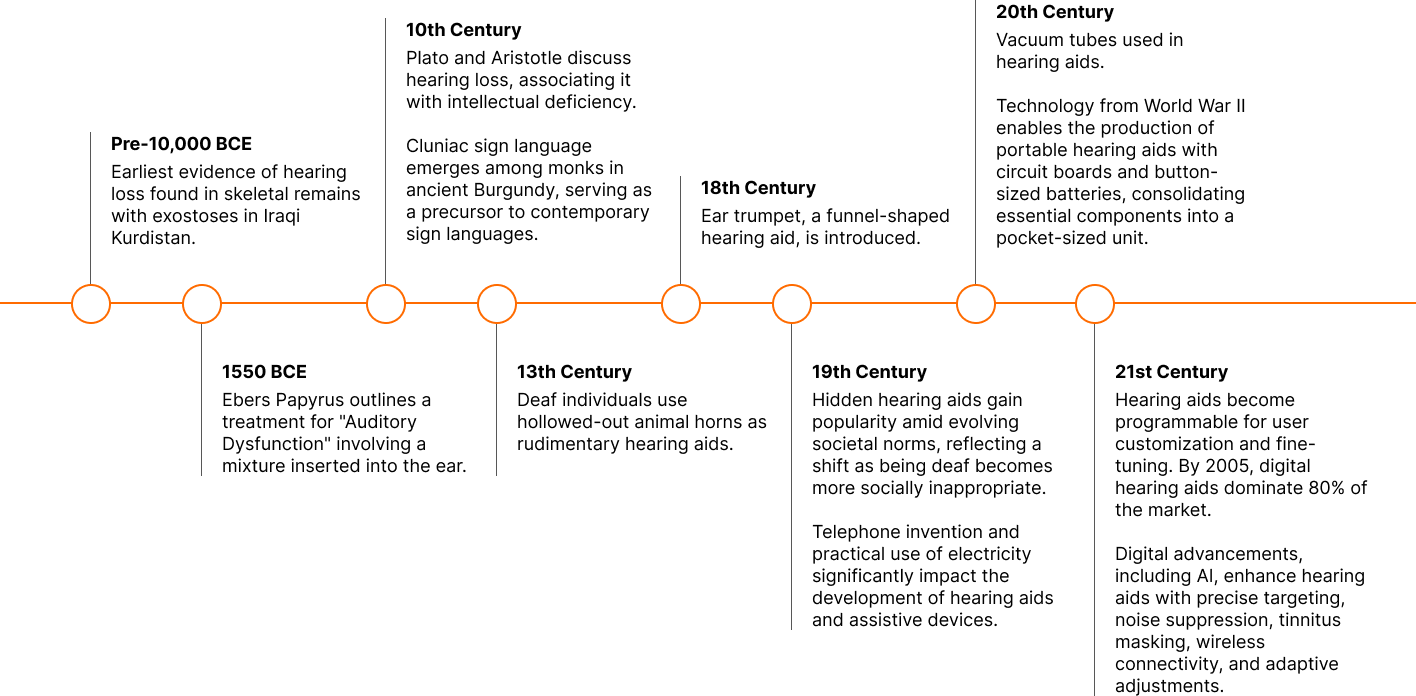
\includegraphics[width=1.0\linewidth]{dissertation/images/timeline.png}    
    \caption{Evolution of Hearing Aid Technology: A historical journey from rudimentary devices in the 13th century to 21st-century digital advancements, including AI integration, transforming the landscape of assistive technology for the Deaf and Hard of Hearing community.}
    \label{fig:timeline} 
\end{figure} 

\section{Existing Technology}
\label{sec:tech}

\subsection{Hearing Aids}

Since the 2000s, hearing aids have been programmable, allowing user customisation and flexibility. By 2005, 80\% of the market was dominated by digital devices, which continued to shrink in size due to advancements in transistor fabrication using silicon. These modern hearing aids seamlessly adapt to different environments and connect with electronic devices like computers and telephones, enhancing accessibility in public spaces \citep{9226670}.

A hearing aid consists of three components: a microphone, amplifier, and speaker. It captures sound, converts it into electrical signals, amplifies them, and relays them to the ear \citep{Disorders_2022}. Designed to alleviate the impacts of hearing loss, hearing aids focus on enhancing speech sounds to improve users' capacity to engage effectively in various situations \citep{ferguson2017hearing}.

The National Institute on Deafness and Other Communication Disorders categorise three primary styles of hearing aids: Behind-the-ear (BTE), In-the-ear (ITE), and Canal aids, which inclue in-the-canal (ITC) and completely-in-canal (CIC). Each addresses different degrees of hearing loss and preferences, offering versatility to users and are displayed in Figure \ref{fig:hearing-aids}. 

Hearing aids utilise analog or digital systems. Analog aids amplify sound waves, with adjustable and programmable options. Digital aids, using numerical codes, provide precise programming, adaptability to frequencies, and advanced features like directional focus. Digital technology, applicable across all types of hearing aids, offers significant customization options for users \citep{Disorders_2022}.

\begin{figure}
    \centering
    \begin{subfigure}[b]{0.2\textwidth}
        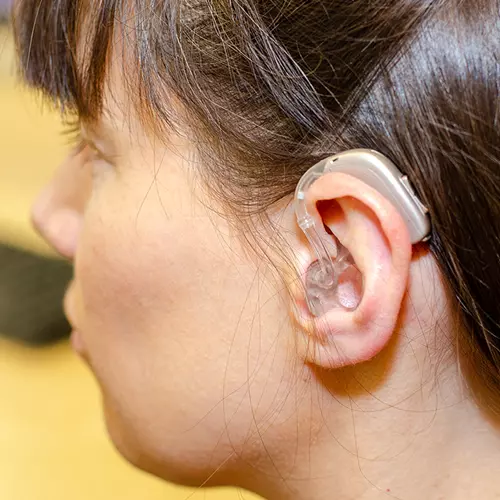
\includegraphics[width=\textwidth]{dissertation/images/BTE.png}
        \caption{Behind the ear (BTE) hearing aid}
        \label{fig:aid1}
    \end{subfigure}
    ~ %add desired spacing between images, e. g. ~, \quad, \qquad, \hfill etc. 
      %(or a blank line to force the subfigure onto a new line)
    \begin{subfigure}[b]{0.2\textwidth}
        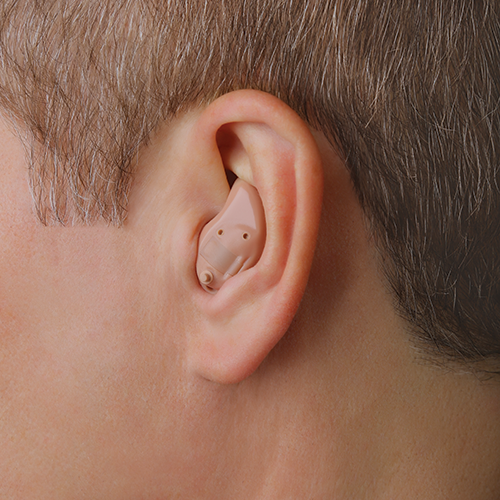
\includegraphics[width=\textwidth]{dissertation/images/ITE.png}
        \caption{In the ear (ITE) hearing aid}
        \label{fig:aid2}
    \end{subfigure}
    \begin{subfigure}[b]{0.2\textwidth}
        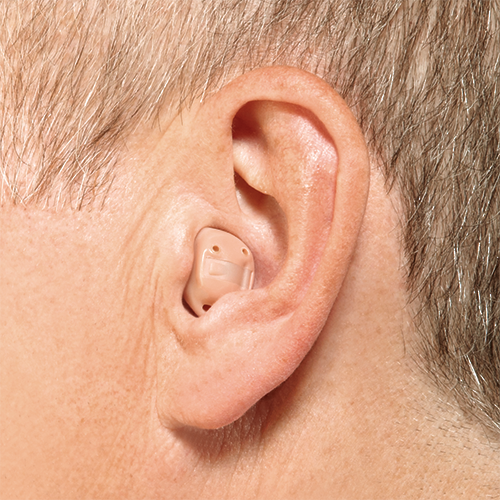
\includegraphics[width=\textwidth]{dissertation/images/ITC.png}
        \caption{In the canal (ITC) hearing aid}
        \label{fig:aid3}
    \end{subfigure}
    ~ %add desired spacing between images, e. g. ~, \quad, \qquad, \hfill etc. 
      %(or a blank line to force the subfigure onto a new line)
    \begin{subfigure}[b]{0.2\textwidth}
        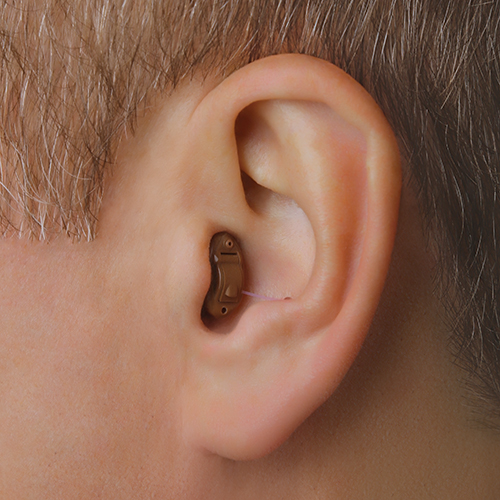
\includegraphics[width=\textwidth]{dissertation/images/CIC.jpg}
        \caption{Completely in canal (CIC) hearing aid}
        \label{fig:aid4}
    \end{subfigure}
    ~ %add desired spacing between images, e. g. ~, \quad, \qquad, \hfill etc. 
    %(or a blank line to force the subfigure onto a new line)   
    \caption{Comparison of Hearing Aid Styles: From Behind-the-Ear (BTE) to In-the-Canal (ITC), illustrating the diverse options for users with varying preferences and hearing needs.}\label{fig:hearing-aids}
\end{figure}

As previously mentioned in Section \ref{sec:motivation}, the hearing aids market is anticipated to continue its upward trajectory \citep{Market_Research_Firm}. This highlights the significance of hearing aids as a vital clinical intervention. However, exploring the landscape of auditory healthcare prompts a critical examination of the accessibility and affordability of these essential devices, particularly considering hearing aid prices detailed in the following tables. This raises important questions about their economic feasibility for a broader demographic.

Multimodal hearing aids represent a transformative advancement in auditory assistive technologies, offering a crucial solution for individuals facing diverse hearing challenges. These next-generation devices seamlessly integrate auditory cues with complementary visual or tactile stimuli, transcending traditional auditory augmentation. They play a pivotal role in restoring intelligibility and reducing cognitive load in noisy environments \citep{shah2022novel}. However, their real-time implementation demands a delicate balance between high data rates, low latency, low computational complexity, and robust security measures \citep{novel}. By strategically combining sensory modalities, multimodal hearing aids aim to provide a more nuanced understanding of the acoustic environment, catering to users with varying degrees of hearing loss. 

\begin{table}[htbp]
    \caption{Hearing Aid Prices in 2024}\label{tab:hearing_aid_prices}
    %\tt 
    \rowcolors{2}{}{gray!3}
    \begin{tabular}{@{}lll@{}}
    %\toprule
    \textbf{Hearing Aid Style} & \textbf{Hearing Aid Price Each (£)} & \textbf{Hearing Aid Price Pair (£)} \\ 
    BTE hearing aid  & 595 & 895 \\ 
    RIC hearing aid  & 595 & 895 \\ 
    ITE hearing aid  & 695 & 1195 \\ 
    CIC hearing aid  & 696 & 1195 \\ 
    ITC hearing aid  & 695 & 1195 \\ 
    IIC hearing aid  & 695 & 1195 \\ 
    BICROS hearing aid  & 795 & NA \\ 
    CROS hearing aid  & 795 & NA \\
    % \bottomrule
\end{tabular}
\end{table}

\begin{table}[htbp]
    \caption{Hearing Aid Price Range in 2024}\label{tab:hearing_aid_price_range}
    %\tt 
    \rowcolors{2}{}{gray!3}
    \begin{tabular}{@{}lll@{}}
    %\toprule
    \textbf{Hearing Aid Budget} & \textbf{Hearing Aid Price Range Singular (£)} & \textbf{Hearing Aid Price Range Pair (£)} \\ 
    Low Budget & 345-695 & 345-695 \\ 
    Basic Budget & 695-895 & 1295-1395 \\ 
    Mid-level Budget & 1095-1195 & 1595-2095 \\ 
    Advanced Budget & 1245-1395 & 2295-2895 \\ 
    Premium Budget & 1595-1695 & 2895-3190 \\
    % \bottomrule
\end{tabular}
\end{table}

In the context of hearing aid affordability, Tables \ref{tab:hearing_aid_prices} and \ref{tab:hearing_aid_price_range} provide an overview of hearing aid prices in 2024. Table \ref{tab:hearing_aid_prices} details the individual and pair prices for various hearing aid styles. Table \ref{tab:hearing_aid_price_range} further categorises hearing aid budgets, outlining the price ranges for singular and pair purchases across different budget tiers: Low Budget, Basic Budget, Mid-level Budget, Advanced Budget, and Premium Budget. This categorisation provides insights into the affordability spectrum within the hearing aid market \citep{Harrison_2024}.

There are many other forms of hearing aids, including implantable hearing aids, such as the middle ear implant (MEI) and bone-anchored hearing aid (BAHA), aim to enhance sound transmission directly into the inner ear. The MEI, attached to a middle ear bone, moves bones to reinforce sound vibrations, while the BAHA, affixed to the bone behind the ear, transmits sound vibrations through the skull, bypassing the middle ear. BAHAs are often used for middle ear issues or unilateral Deafness. However, the need for surgical implantation raises concerns among specialists who assess potential benefits against associated risks \citep{Disorders_2022}.

\subsection{Speech Recognition}
\label{sec:speech-recog}

The history of speech recognition, and automated speech recognition (ASR), traces its roots back to the 1920s, where "Radio Rex," a celluloid dog animated by a spring release triggered by the vocal cue "Rex", which is 500 Hz acoustic energy. This toy demonstrated the first innovations in speech recognition technology \citep{david1962eyes}. From this, ASR has evolved into a sophisticated Natural Voice-Voice Interface (VUI). Present-day applications span a spectrum of utilities, including communication with smart home appliances, personal assistants, and cellphones, particularly catering to the elderly \citep{song2022investigation}. Furthermore, ASR plays a pivotal role in general transcription, generating automatic captions for audio or video text, and significantly contributes to augmentative communication for individuals with disabilities \citep{semary2024using}.

Jurafsky, \citep{jurafskyspeech}, provides an insightful exploration of ASR dimensions, including vocabulary size, speaker interactions, channel and noise conditions, and speaker-class characteristics. Complexities escalate with open-ended tasks like transcribing videos or human conversations, variations in channel and noise, and the nuanced impact of speaker characteristics such as regional accents. Furthermore, Jurafsky outlines the encoder-decoder architecture of speech recognition, beginning with the user speaking and producing an initial audio signal. This signal is then captured, undergoing pre-processing for noise reduction and enhancement. Relevant features are extracted using techniques like MFCCs, transformed into feature vectors for analysis. Acoustic modeling, often with HMMs or neural networks, establishes the relationship between features and phonetic units. Language modeling adds context, refining word sequence likelihood. Decoding combines acoustic and language models, utilizing algorithms like Viterbi decoding. Post-processing refines text using statistical language models and grammatical constraints, ensuring accuracy. The final output is transcribed text or commands, representing the user's spoken input. Figure \ref{fig:ASR} displays a simplified version of the ASR architecture. 

\begin{figure}
    \centering
    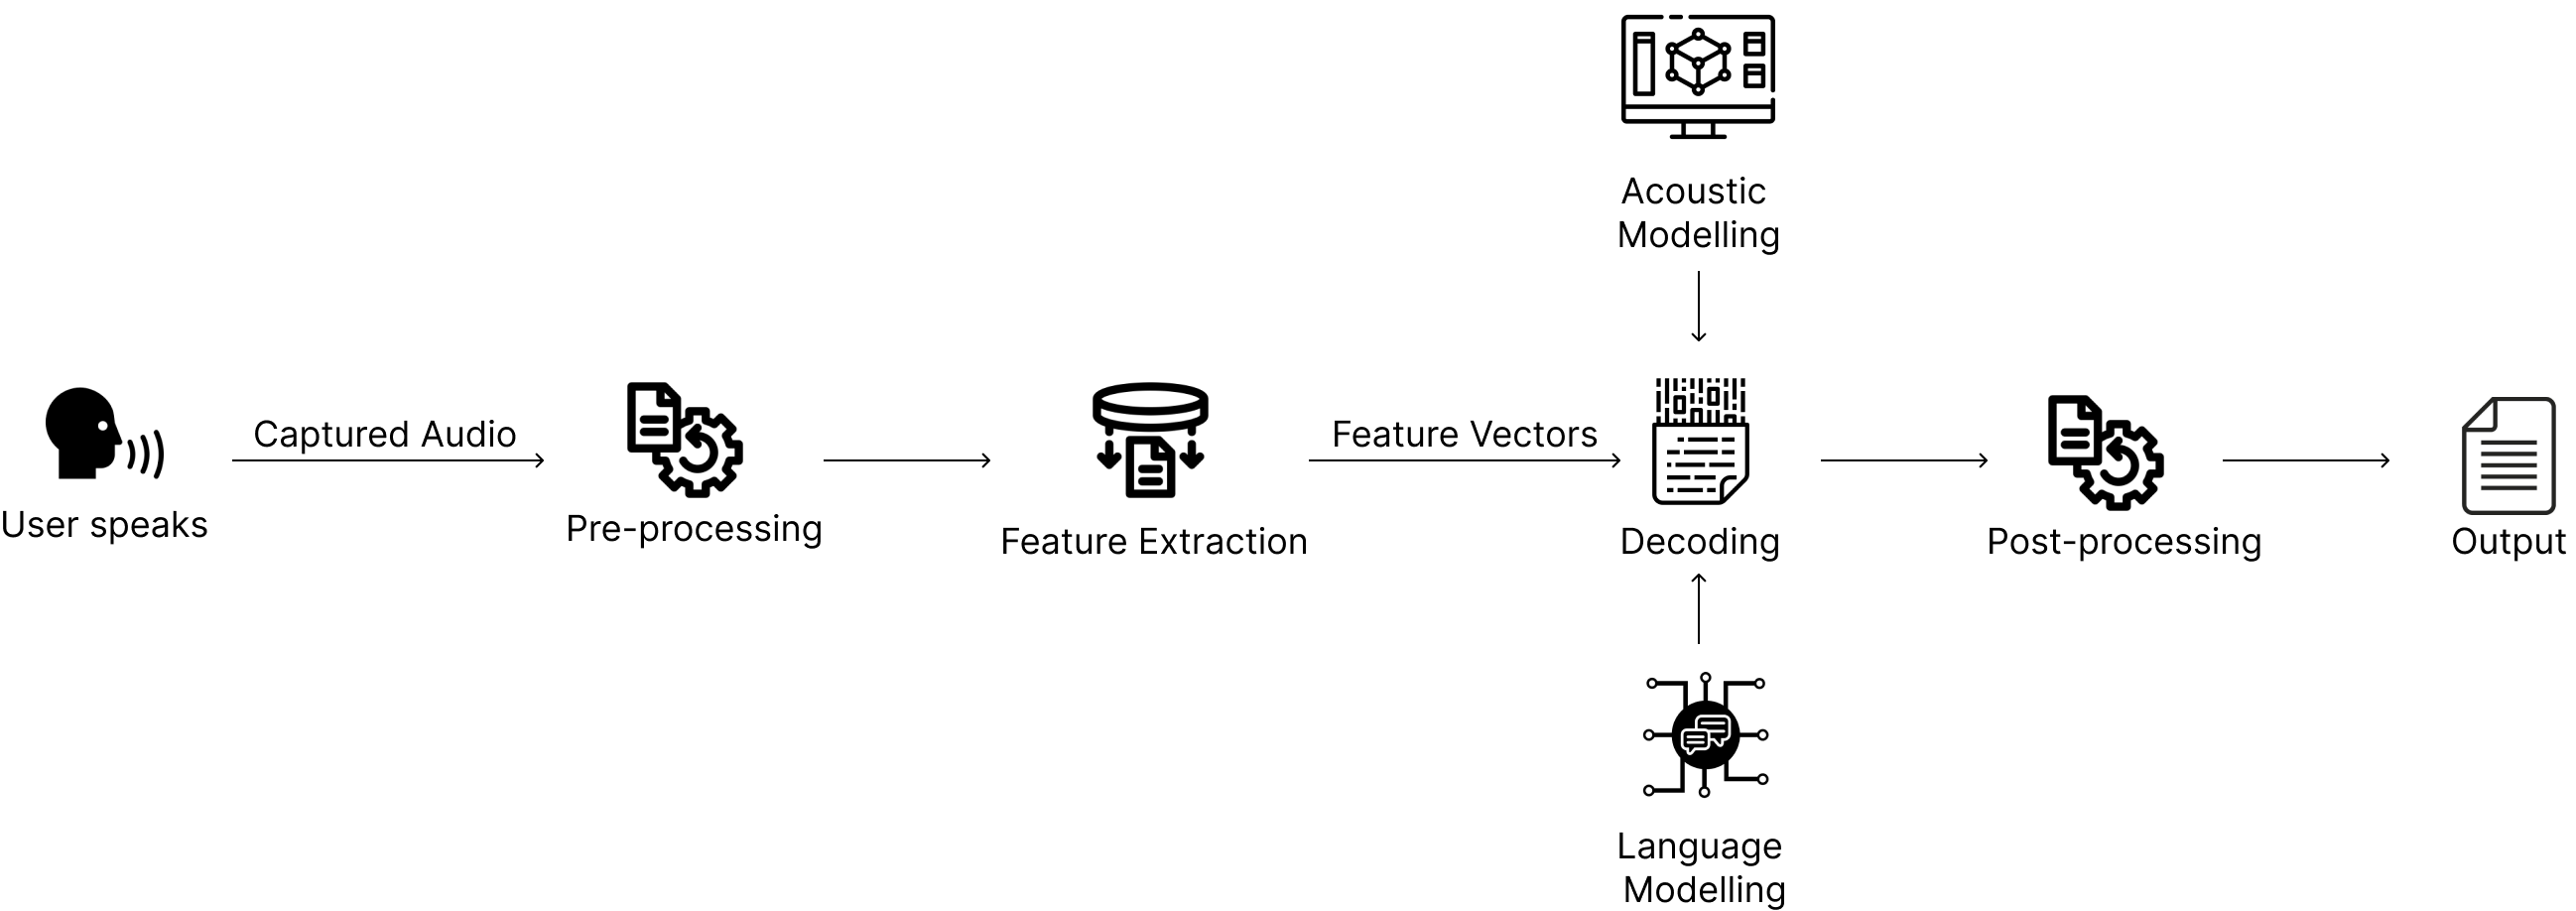
\includegraphics[width=1.0\linewidth]{dissertation/images/ASR.png}    
    \caption{Flow Diagram of Speech Recognition Process: From User Speech Input to Accurate Transcription}
    \label{fig:ASR} 
\end{figure} 

Table \ref{tab:ASR} presents a comprehensive overview of Word Error Rates (WER\%) and Character Error Rates (CER\%) across diverse speech recognition tasks in American English and Mandarin Chinese. Reflecting the accuracy of ASR systems, these rates fluctuate across tasks, with lower percentages indicative of heightened accuracy and efficiency in transcription \citep{jurafskyspeech}. This consolidated analysis underscores the evolving landscape of ASR and its crucial role in contemporary technological applications.

\begin{table}[htbp]
    \caption{Word Error Rates (WER\%) and Character Error Rates (CER\%) across diverse speech recognition tasks in American English and Mandarin Chinese}\label{tab:ASR}
    %\tt 
    \rowcolors{2}{}{gray!3}
    \begin{tabular}{@{}ll@{}}
    %\toprule
    \textbf{English Tasks} & \textbf{WER\%} \\ 
    LibriSpeech audiobooks 960hour clean &  1.4 \\ 
    LibriSpeech audiobooks 960hour other &  2.6 \\ 
    Switchboard telephone conversations between strangers &  5.8 \\ 
    CALLHOME telephone conversations between family & 11.0 \\ 
    Sociolinguistic interviews, CORAAL (AAL) & 27.0 \\
    CHiMe5 dinner parties with body-worn microphones & 47.9 \\
    CHiMe5 dinner parties with distant microphones & 81.3 \\
    \textbf{Chinese (Mandarin) Tasks} & \textbf{CER\%} \\
    AISHELL-1 Mandarin read speech corpus & 6.7 \\
    HKUST Mandarin Chinese telephone conversations & 23.5 \\
    % \bottomrule
\end{tabular}
\end{table}

Advancements in speech recognition technology are empowering individuals, particularly those with disabilities, to seamlessly control devices, access information, execute tasks, and interact with digital platforms. This progress not only fosters independence but also enhances overall quality of life by providing newfound convenience and accessibility. For people with disabilities, such as those with mobility or visual disabilities, speech recognition serves as a vital tool, enabling them to navigate digital interfaces and perform tasks that may have been challenging or impossible otherwise. By offering voice-controlled alternatives to traditional input methods, speech recognition technology enables individuals with disabilities to participate more fully in various aspects of daily life, bridging the gap between accessibility and inclusivity in the digital realm \citep{semary2024using}. However, there are still some minority biases within speech recognition systems. 

Many individuals become frustrated using technology such as Siri and even stop using them due to its Americanisation, which made it unable to recognise their speech. This illustrates the challenges faced by individuals with non-American names or accents. Many studies corroborates these concerns, revealing significant racial disparities in ASR technologies like Siri, with non-white speakers being disproportionately misunderstood \citep{koenecke2020racial}. This bias not only erases cultural and linguistic identities but also poses challenges for individuals with disabilities who rely on voice recognition tools. Addressing these biases demands a multifaceted approach, including incorporating diverse training data, extensive product testing, and fostering diversity within tech companies' workforces. Moreover, tech companies need to recognise the influence of market-driven decisions on the prioritisation of inclusive technology development to mitigate these biases effectively \citep{Lopez-Lloreda_2020}.

\subsection{Speech Synthesis}
\label{sec:speech-syn}

The historical narrative of speech synthesis technology traces back to Wolfgang von Kempelen's pioneering efforts in the 18th century, where he developed rudimentary methods using delicate bellows, springs, and resonance boxes to synthesize simple words. Despite these early attempts, the intelligibility of the synthesized speech remained poor. However, von Kempelen's innovations laid the groundwork for modern text-to-speech (TTS) synthesis, which involves mapping text to acoustic waveforms. Today, TTS technology plays crucial roles in conversational agents, aids for Blind individuals, and communication tools for individuals with neurological disorders \citep{jurafskyspeech, klatt1980software}.

Jurafsky continues to explain the contemporary objective of speech synthesis, often referred to as text-to-speech or TTS, involves the inverse process compared to ASR. It aims to transform textual inputs into corresponding waveforms, a technological imperative with applications spanning dialogue systems, gaming interfaces, and educational tools. TTS systems, like their ASR counterparts, predominantly adopt the encoder-decoder architecture, leveraging either Long Short-Term Memory networks (LSTMs) or Transformers.

A distinctive characteristic in the training paradigm distinguishes TTS from ASR. While ASR systems prioritise speaker independence, necessitating training on diverse datasets with contributions from numerous speakers, TTS systems often embrace speaker dependence. For instance, the LJ Speech Corpus, a widely used dataset, comprises 24 hours of recordings from a singular speaker, emphasizing the feasibility of consistent voice generation with comparatively smaller datasets.

The TTS process unfolds in two pivotal components: an encoder-decoder model for spectrogram prediction, mapping text to mel spectrographs, and a vocoder, responsible for generating waveforms from mel spectrograms. In parallel, TTS systems undergo a crucial first pass of text normalization preprocessing to handle non-standard words, including numbers and abbreviations. This initial normalization step is vital given the verbalization differences compared to their spelled counterparts. Although modern end-to-end TTS systems exhibit the capacity to learn some normalization during training, the inherent limitation in training data size necessitates a distinct normalization step. This normalization can be achieved through rule-based approaches or an encoder-decoder model.

Crucially, the evaluation of speech synthesis systems remains a domain predominantly influenced by human listeners. This assessment involves playing synthesized sentences to listeners, who provide mean opinion scores (MOS) or participate in AB tests. The human-centric evaluation approach underscores the nuanced and subjective nature of assessing the quality of synthesized speech, prompting ongoing research in search of automated metrics to complement or potentially replace human evaluations.

In tandem with the advancements in speech recognition, speech synthesis has undergone rapid evolution propelled by new models, particularly those rooted in deep learning \citep{klatt1980software}. These developments are progressively closing the gap, aiming to achieve speech synthesis that is virtually indistinguishable from human speech \citep{tan2024naturalspeech}.

\section{Other Technology}
\label{sec:other}

The landscape of assistive technology has been significantly shaped by the integration of accessibility features in contemporary smartphones, exemplified by prominent brands such as Apple, Android/Google Pixel, and Samsung Galaxy.

Apple has been a trailblazer in this domain, incorporating a robust set of accessibility features in its iOS devices, including VoiceOver for screen reading, magnification gestures, AssistiveTouch for motor challenges, and their beta feature for live captions \citep{AppleSupport}. Unfortunately, the majority of these advanced features are only available on iOS17, rendering them incompatible with iPhone models preceding the iPhone 8. This presents a significant barrier to access, effectively pricing out users who wish to utilise these capabilities, as they would be compelled to invest in a new phone that supports the latest iOS version.

Android, particularly on Google Pixel devices, has followed suit with its commitment to inclusivity, offering features like TalkBack, Live Transcribe, Sound Amplifier, and being able to connect hearing aids to your device to enhance usability for individuals with diverse needs \citep{Google}. Samsung Galaxy phones have also made strides in accessibility, featuring Voice Assistant, Screen Reader, Hearing Aid Compatibility, and sound amplification to cater to users with visual and hearing loss \citep{Samsung_uk_2023}. The collective efforts of these technology giants underscore a commitment to creating inclusive digital ecosystems, ensuring that individuals of varying abilities can seamlessly integrate smartphones into their daily lives.

%==================================================================================================================================
\chapter{Use Cases \& Requirements}
\label{sec:use-cases-and-req}
% What is the problem that you want to solve, and how did you arrive at it?
% Make it clear how you derived the constrained form of your problem via a clear and logical process.

\section{User Cases}
\label{sec:user-cases}

% list off different types of hearing loss and how the web-app accomodates them 
% e.g. people who are completely deaf cannot use the hearing aid feature, but they can still use the speech-to-text for captions and text-to-speech to type and speak to others

This section details varied hearing loss categories and how the web app accommodates them. Acknowledging complete Deafness limitations, it highlights alternatives like speech-to-text and text-to-speech for effective communication. Through concise user cases, it ensures a nuanced understanding of the app's inclusivity and usability across different hearing loss.

\textbf{User with Partial Hearing Loss}
\begin{itemize}
    \item Utilises speech-to-text for improved communication
    \item Integrated text-to-speech feature with speech-to-text for clearer communication
    \item Accesses the hearing aid functionality for audio playback
    \item Engages with text-to-speech for communication if uncomfortable with speech
\end{itemize}

\textbf{User with Profound Hearing Loss, who may be Non-Verbal}
\begin{itemize}
    \item Utilises speech-to-text for captions
    \item Engages with text-to-speech for communication
\end{itemize}

\textbf{User Seeking Customisation}
\begin{itemize}
    \item Adjusts hearing aid settings based on personal preferences
    \item Customises the user interface for a personalised experience
    \item Logging into user account to save individualised settings
\end{itemize}

\textbf{User in Multilingual Settings}
\begin{itemize}
    \item Utilises language customisation in speech recognition and synthesis
    \item Engages with the application in their preferred language
\end{itemize}

\textbf{Collaborative Users}
\begin{itemize}
    \item Engages in collaborative features, such as sharing messages
    \item Provides feedback and contributes to the improvement of the platform
\end{itemize}

\textbf{Users on Various Devices}
\begin{itemize}
    \item Accesses the web app seamlessly across smartphones, tablets, laptops, smartwatches, Raspberry Pi, and desktops
    \item Ensures consistent functionality on different operating systems
\end{itemize}

\textbf{New Users}
\begin{itemize}
    \item Navigates through an intuitive user interface designed for user-centric experience
    \item Benefits from user-friendly onboarding processes
\end{itemize}

\section{Functional and Non-Functional Requirements}
\label{sec:req}

Throughout the project's evolution, initial requirements aimed at real-time sound amplification, alongside edge computing for additional functionalities like user information management, speech recognition, and synthesis. However, as our research deepened and time constraints became apparent, we made strategic decisions to streamline our focus.

We recognised the necessity to refine our objectives, prioritising core functionalities while leaving behind more ambitious features that could be taken forward in future projects. Consequently, we opted for a simplified approach, substituting real-time amplification with a more manageable frequency cut-off mechanism along-side gain and Q value adjustment, enabling users to manipulate sound waves effectively through their earbuds. Additionally, instead of delving into intricate edge computing processes, we simplified the architecture to incorporate essential elements through API calls.

By aligning our project goals with practical considerations, we ensure efficient resource utilisation and a more targeted development process. This strategic pivot allows us to deliver a robust solution within our constraints while maintaining a high standard of functionality and usability.

The requirements for the web-app were categorised by employing the MoSCoW method \citep{Business}, an Agile Business Consortium prioritization technique. This method involves labeling requirements based on their priority:

\begin{itemize}
    \item \textbf{Must Have:} Critical requirements essential for creating a minimum viable solution.
    \item \textbf{Should Have:} Important requirements that are not critically essential.
    \item \textbf{Could Have:} Desirable requirements acceptable if not implemented.
    \item \textbf{Won’t Have this Time:} Requirements out of the current project's scope but could be considered for future implementation.
\end{itemize}

Functional requirements are denoted by (\textbf{F}), while non-functional requirements are indicated by (\textbf{NF}).

\textbf{Must have (MH)}
\begin{enumerate}[{MH}.1]
  \item Speech-to-text (\textbf{F}): The web app must support speech-to-text functionality for generating captions.
  \item Text-to-speech (\textbf{F}): It must include text-to-speech features for effective communication.
  \item User interface (\textbf{F}): The app must have an intuitive and accessible user interface.
  \item Hearing aid (\textbf{F}): Audio playback in the web app is a critical feature for users with partial hearing loss.
\end{enumerate}

\textbf{Should Have (SH)}
\begin{enumerate}[{SH}.1]
  \item Customisable Settings (\textbf{F}): Implement customisable variables to all audio outputs.
  \item User Feedback (\textbf{F}): Include an option for users to provide feedback on the app's usability, allowing continuous improvement.
  \item Device Compatibility (\textbf{NF}): Ensure compatibility with various devices, including smartphones, tablets, and desktops.
  \item User Profiles (\textbf{F}): The web app should offer user profiles to save personalised settings.
  \item Language Settings (\textbf{F}): Allow for multiple language options for speech recognition and synthesis.
\end{enumerate}

\textbf{Could Have (CH)}
\begin{enumerate}[{CH}.1]
  \item Integration with Other Technologies (\textbf{F}): Explore integration with additional assistive technologies for a comprehensive user experience.
  \item Collaboration Features (\textbf{F}): Allow users to share experiences or tips on using the app, fostering a sense of community.
  \item Regular Updates (\textbf{F}): Continuous improvement through regular updates based on user feedback.
\end{enumerate}

\textbf{Won’t Have this Time  (WH)}
\begin{enumerate}[{WH}.1]
  \item Proprietary Hardware Support (\textbf{F}): Integration with proprietary, expensive hardware for hearing aid support is out of scope.
  \item Complex Features (\textbf{F}): Features requiring extensive resources, such as speaker recognition and siren detection, are not prioritised.
\end{enumerate}

%==================================================================================================================================
\chapter{Design}
\label{sec:design}
% How is this problem to be approached, without reference to specific implementation details? 

% Design should cover the abstract design in such a way that someone else might be able to do what you did, but with a different language or library or tool.

\section{Architectural Design}
\label{sec:arch-design}

In designing the architecture for the assistive web application, careful consideration was given to ensuring our project aims outlined in Section \ref{sec:aims} are met. The following details the architectural components and decisions made during the design phase to meet the requirement MH.3 aforementioned in Section \ref{sec:req}.

\begin{figure}
    \centering
    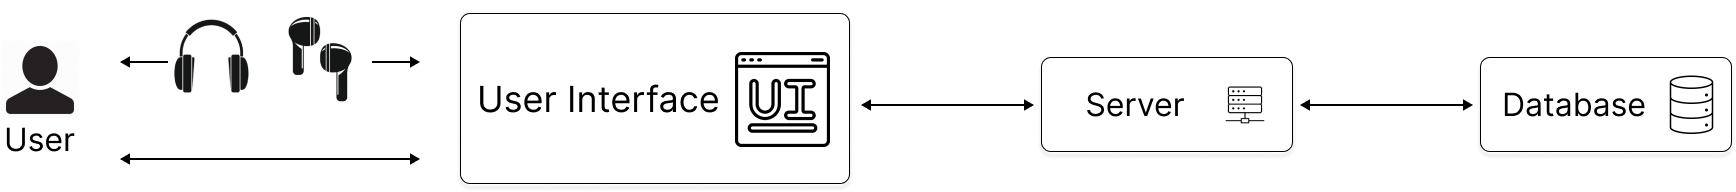
\includegraphics[width=\linewidth]{dissertation/images/architecture.png}    
    \caption{Architectural Design Overview: A visual representation of the client-server architecture and communication protocols underlying the development of the assistive web application.}
    \label{fig:architecture} 
\end{figure}

The client-side architecture, built on React TypeScript (TSX) \footnote{\url{https://www.typescriptlang.org/docs/}}, fosters a dynamic and responsive user interface. Users can interact directly with the interface or connect an audio device to unlock additional audio features. Leveraging React TSX's component-based design, development remains modular, enhancing both reusability and maintainability. On the server side, operations are driven by a Node.js server, delivering an event-driven and scalable backend. This server hosts the React TSX application and manages requests, facilitating seamless communication between client and server. Secure storage of user preferences in a database enables personalized experiences across the platform.

Communication between the client and server is achieved through RESTful APIs \citep{Red-Hat}. This approach simplifies data exchange and ensures interoperability. Users experience a smooth interaction with the application, and future integrations are facilitated by the adherence to RESTful principles.

Security stands as a paramount concern within the architectural design, given the prevalent risks associated with potential eavesdropping on conversations through device microphones, owing to their system access permissions \citep{kroger2019my}. HTTPS secures communication, preventing unauthorized access to sensitive data. User preferences will be encrypted before storage, and robust authentication and authorization mechanisms are implemented to protect user accounts.

The deployment strategy involves running the React TSX application on a server. GitHub Pages encapsulates the application and its dependencies, providing a consistent environment. This ensures ease of deployment and scalability. Future scalability needs are addressed through horizontal scaling, leveraging load balancing techniques as displayed in Figure \ref{fig:architecture}.

\section{Affordability}
\label{sec:affordability}

As outlined in Section \ref{sec:aims}, the primary aim of the application is to provide its services completely free of charge, aligning with Project Aim PA.1, with only minimal hardware required. By offering essential assistive technologies for the Deaf and Hard-of-Hearing community without extortionate financial barriers, the platform ensures accessibility to all individuals, regardless of their economic status as mentioned in Section \ref{sec:motivation}. However, as outlined in Section \ref{sec:tech}, contemporary technology, particularly hearing aids, often carries a heavy price tag, with the most affordable option starting at £345. Upon navigating through the Currys website \footnote{Currys operates as a retailer specialising in technology products: \url{https://www.currys.co.uk/}}, we identified significantly more budget-friendly alternatives that can access the outlined assistive web-app. The lowest-priced smartphone equipped with browser accessibility is priced at just £59 \footnote{\url{https://www.currys.co.uk/products/xiaomi-redmi-a2-32-gb-black-10250273.html}}, while the least expensive earbuds are available for a mere £3.97 \footnote{\url{https://www.currys.co.uk/products/skullcandy-jib-headphones-black-10178565.html}}. Remarkably, this combination totals £282.03 less than the cheapest hearing aids on the market.

\section{User Interface (UI) Design}
\label{sec:UI}

Although assistive technologies have many beneficial features, there are instances where users discontinue their usage. For hearing aids, research has indicated abandonment rates reaching up to 78\% \citep{scherer1996outcomes}. Factors contributing to this rate of abandonment encompass issues associated with the device itself, including malfunctions or aesthetic considerations \citep{ijerph18147259}. Hence why this project aims to be inclusive and user-centric in it's UI design. 

In crafting the User Interface (UI) for the assistive web application, paramount consideration was given to ensure user-friendliness and accessibility. The design principles not only prioritise ease of use but also cater to the unique needs of Deaf and Hard-of-Hearing users. Particularly being mindful of the fact that around 25\% of individuals aged over 60 years grapple with hearing loss, underscoring the significance of this challenge among older adults \citep{haile2021hearing}.

In software development, UI design holds a crucial role, serving as a pivotal element in meeting user expectations and maximizing the software's functionality. A well-crafted UI not only enhances user acceptance of the software but also plays a vital role in educational contexts. For instance, an effective UI in educational software can significantly improve users' engagement with and absorption of knowledge \citep{chu1998evolution}. Users rely on the feedback provided by the UI interface to shape their learning experiences, emphasizing the substantial impact of UI design on the overall user interaction with educational software.

In adherence to the foundational principles of User Interface Design Basics \citep{Usability.gov_2014}, the wireframe design for the web application was meticulously crafted with a focus on key elements:
\begin{enumerate}[{UI}.1]
    \item \textbf{Simplicity in Interface:} The decision to employ a single-page web application was deliberate, aiming to ensure all features remain straightforward and user-friendly.
    \item \textbf{Consistency with Common UI Elements:} Consistent CSS styling for common interface elements was implemented, fostering a sense of comfort and familiarity for users across the web application.
    \item \textbf{Purposeful Page Layout:} The centralization of features within the layout strategically directs attention to vital information, enhancing overall user experience.
    \item \textbf{Strategic Use of Color and Texture:} Thoughtful selection of colors, appealing to users and promoting a comfortable interaction with the web application, potentially contributing to user retention.
    \item \textbf{Typography for Hierarchy and Clarity:} Incorporation of varying font sizes for text boxes, especially considering potential users from the elderly demographic, enhances hierarchy and readability.
    \item \textbf{Clear Communication of System Status:} Implementation of error communication strategies and provision of a user guide contribute to effective user-system communication.
    \item \textbf{Consideration of Defaults:} The establishment of default settings caters to the needs of new users, streamlining their initial interaction with the web application.
\end{enumerate}

\begin{figure}
    \centering
    \begin{subfigure}[b]{0.60\textwidth}
        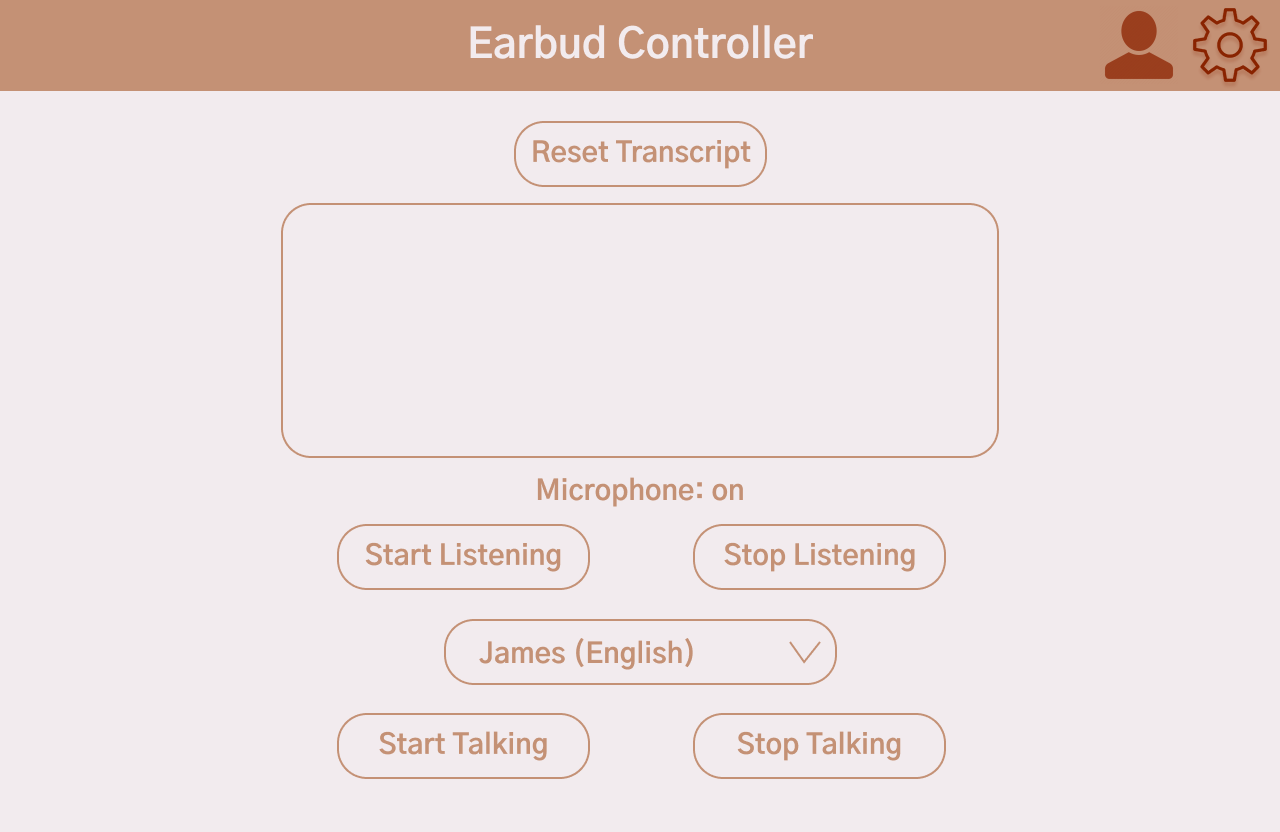
\includegraphics[width=\textwidth]{dissertation/images/Home.png}
        \caption{Wireframe design for the single-page web application, meticulously crafted for a user-centric and inclusive experience}
        \label{fig:home}
    \end{subfigure}
    ~ %add desired spacing between images, e. g. ~, \quad, \qquad, \hfill etc. 
      %(or a blank line to force the subfigure onto a new line)
    \begin{subfigure}[b]{0.30\textwidth}
        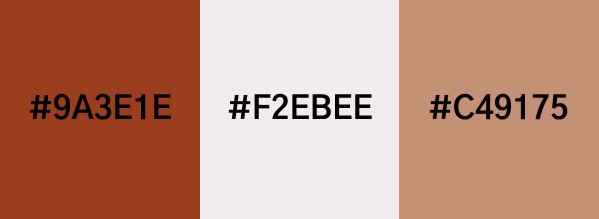
\includegraphics[width=\textwidth]{dissertation/images/colours.png}
        \caption{Thoughtfully chosen color palette for the web application, ensuring a visually appealing and user-friendly interface for diverse users.}
        \label{fig:colours}
    \end{subfigure}
    ~ %add desired spacing between images, e. g. ~, \quad, \qquad, \hfill etc. 
    %(or a blank line to force the subfigure onto a new line)    
    \caption{A comprehensive wireframe design for the single page web-app \subref{fig:home}, coupled with a carefully curated color palette \subref{fig:colours}, harmonizing aesthetics and usability for an inclusive user experience.}
    \label{fig:wireframe}
\end{figure}

Leveraging the capabilities of Figma, we crafted the wireframe that serves as the blueprint for the single-page web application as seen in Figure \ref{fig:home}. Adhering to the established principles of User Interface Design \citep{Usability.gov_2014}, the wireframe design strategically centers features to guide user attention effectively. The color palette, depicted in Figure \ref{fig:colours}, was meticulously curated with three warm tones – brown, off-white, and pink – to ensure a visually comfortable and user-friendly experience. Grounded in color-emotion associations and preferences, these warm hues align with positive sentiments of friendliness, comfort, reassurance, and liveliness \citep{UIcolor}. The selection of brown, off-white, and pink is further justified by their favorable rankings in Liao's research, reinforcing the intent to create an emotionally resonant and engaging web-app interface.

\section{User Experience (UX) Design}
\label{sec:UX}

UX design revolves around a deep understanding of user needs, values, and limitations, aligning with overarching business objectives. In crafting the UX for the assistive web application, the focus is on a user-centric approach. This ensures a seamless and inclusive interaction tailored to varying degrees of hearing loss. Key principles include accessibility, ease of use, and overall satisfaction, fostering a positive and engaging user experience throughout \citep{usabilityUX}.

In aligning with the foundational principles of the User Experience Honeycomb \citep{Morville_2004}, the web application's design is meticulously tailored, emphasizing key elements:
\begin{enumerate}[{UX}.1]
    \item \textbf{Useful:} The web app's content is meticulously curated to provide affordable and effective solutions for the diverse needs of the Deaf and Hard-of-Hearing community. Features such as speech-to-text, text-to-speech, and adaptive settings contribute to the practicality and usefulness of the application.
    \item \textbf{Usable:} Through the implementation of a single-page design, the web app prioritizes simplicity and intuitive interaction. The user interface is thoughtfully structured, allowing users to navigate seamlessly between features, ensuring a user-friendly experience for individuals of varying technological proficiencies.
    \item \textbf{Desirable:} The design incorporates visually appealing elements, such as warm and comforting colors, ensuring a positive emotional impact on users. The user interface is crafted to be aesthetically pleasing, fostering a sense of familiarity and comfort during interaction.
    \item \textbf{Findable:} The web app emphasizes navigability, with clear and well-organized menus and sections. Users can easily locate and access desired features, ensuring a straightforward and efficient search and interaction process.
    \item \textbf{Accessible:} Accessibility is a core principle, with features designed to cater to users with diverse hearing loss. The web app includes options for customization, font-size adjustments, and other accessibility settings to enhance usability for all users.
    \item \textbf{Credible:} The web app establishes credibility through transparent communication, clear error handling, and user guides. By providing reliable and accurate information, the application builds trust and confidence among users.
    \item \textbf{Valuable:} The web app's value proposition lies in its commitment to delivering meaningful and accessible assistive solutions. Regular updates, user engagement studies, and responsiveness to user feedback ensure continuous improvement aligned with the mission of enhancing the user experience and meeting the unique needs of the target audience.
\end{enumerate}

%==================================================================================================================================
\chapter{Implementation}
\label{sec:implementation}
% What did you do to implement this idea, and what technical achievements did you make?

\section{Chosen Technologies}

Figma was chosen for wireframe development due to its versatile and collaborative features. This cloud-based design platform enables real-time collaboration, concurrent editing, and seamless transitions from wireframing to prototyping.

React with TypeScript (TSX) has been chosen as the front-end framework for the development of this web application. Leveraging TypeScript's static typing ensures enhanced code quality and reduces the occurrence of runtime errors. The component-based architecture of React simplifies the process of user interface (UI) development, providing a dynamic and responsive user experience to fulfill the MH.3 requirement outlined in Section \ref{sec:req}. Utilising React provides us with the capability to fulfill SH.3, as the web-app is accessible on any device with a web browser. We even verified this functionality by successfully testing it on a Raspberry Pi.

Node.js serves as the selected back-end framework, responsible for handling server-side operations and facilitating interactions with the chosen database. Its asynchronous, non-blocking I/O capabilities make it well-suited for managing concurrent connections, thereby ensuring optimal performance and responsiveness for user requests.

The database system utilised for storing user preferences and relevant data is Clerk. This choice aligns with the project's requirements, offering robust capabilities for user authentication. Clerk's implementation ensures a secure and seamless user experience, addressing the authentication needs of the web application effectively.

For audio processing, the project integrates two fundamental technologies: Web Speech API and Web Audio API. These APIs empower the web application with features such as speech-to-text, text-to-speech, and audio playback to fulfill the MH.1, MH.2, and MH.3 requirements respectively, as aforementioned in Section \ref{sec:req}. The Web Speech API facilitates accurate and efficient speech recognition, while the Web Audio API enhances audio processing capabilities, ensuring a seamless and high-quality user experience.

Several security measures have been implemented to safeguard user data and uphold a secure user experience. The utilisation of HTTPS ensures encrypted data transmission, mitigating potential security risks with easedropping \citep{kroger2019my}. Additionally, Clerk's robust user authentication mechanisms contribute to the overall security posture of the web application.

To establish the web application's public accessibility, the selection of an appropriate hosting platform was imperative. GitHub Pages emerged as the preferred choice due to its provision of free static website hosting, comparable to alternatives like Netlify, Cloudflare and Render, which were all contemplated during the project's planning phase. These platforms offer streamlined integration with Git version control, ensuring collaborative development and effective change tracking. GitHub Pages, integral to the GitHub ecosystem utilised for repository hosting, brings the advantage of seamless integration with other GitHub features streamlining the development workflow. Although we did create a Jira board for managing issues \footnote{\url{https://www.atlassian.com/software/jira}}. Notably, GitHub Pages supports custom domain usage, enabling the utilisation of a personalised domain name for the website. Furthermore, GitHub fosters a sense of community where users can collaborate and leave feedback. This technology allows for the project to fulfill the CH.2 and CH.3 features outlines in Section \ref{sec:req}.

During the course of this project, the WH.2 requirement outlined in Section \ref{sec:aims} was thoroughly researched and initial implementation efforts commenced utilising Picovoice Eagle \citep{PicovoiceWordmark}. Despite the availability of numerous examples for implementation, akin to web development practices, the model provided failed to function as expected. Subsequently, upon contacting the company to address a potential bug in the model, no response was received. Although this feature can potentially be a stepping stone for real-time captioning to distinguish between speakers, the priority of this feature was downgraded within the project's requirements priorities due to the bugs present. 

\section{Technological Stack}
\label{sec:tech-stack}

% Frontend: React for the user interface.
% Backend: Node.js and Express for server-side logic.
% Speech Processing: Integration of the Web Speech API for text-to-speech and speech-to-text capabilities.

It is important to note that, throughout the project, I implemented verbal code reviews with fellow Computing Science students after developing each feature. This helped to catch bugs and improve code readability. It also provided valuable learning opportunities, allowing reviewers to familiarise themselves with the codebase and learn new technologies and techniques. Overall, code reviews fostered a collaborative environment for continuous improvement and skill development to produce a better project \citep{Atlassian}.

\subsection{Web Speech API}
\label{sec:web-speech-API}

Following our aims and requirements of the web-app in Sections \ref{sec:aims} and \ref{sec:req}, we identify Web Speech API to be the ideal method of providing precise and accurate speech recognition and speech synthesis. The Web Speech API empowers the integration of voice data into web applications, consisting of two primary components:  SpeechRecognition for Speech-to-Text and SpeechSynthesis for Text-to-Speech \citep{MozDevNet_2023}. 

The functionality of the Web Speech API's speech recognition involves capturing speech through a device's microphone to facilitate real-time conversion of spoken language into written text, offering precise and responsive speech-to-text capabilities within the web application. This input is streamlined through the SpeechRecognition interface, which interprets voice content from an audio input. The interface's constructor is utilised to instantiate a new SpeechRecognition object, equipped with diverse event handlers for detecting speech input from the device's microphone. Additionally, the SpeechGrammar interface serves as a container for a specific grammar set that the application should recognise, defined using JSpeech Grammar Format (JSGF). Essentially the vocabulary designated for recognition in a specific application. Upon successful recognition of a word or phrase, the result is returned in the form of a text string, triggering subsequent actions.

\begin{figure}
    \centering
    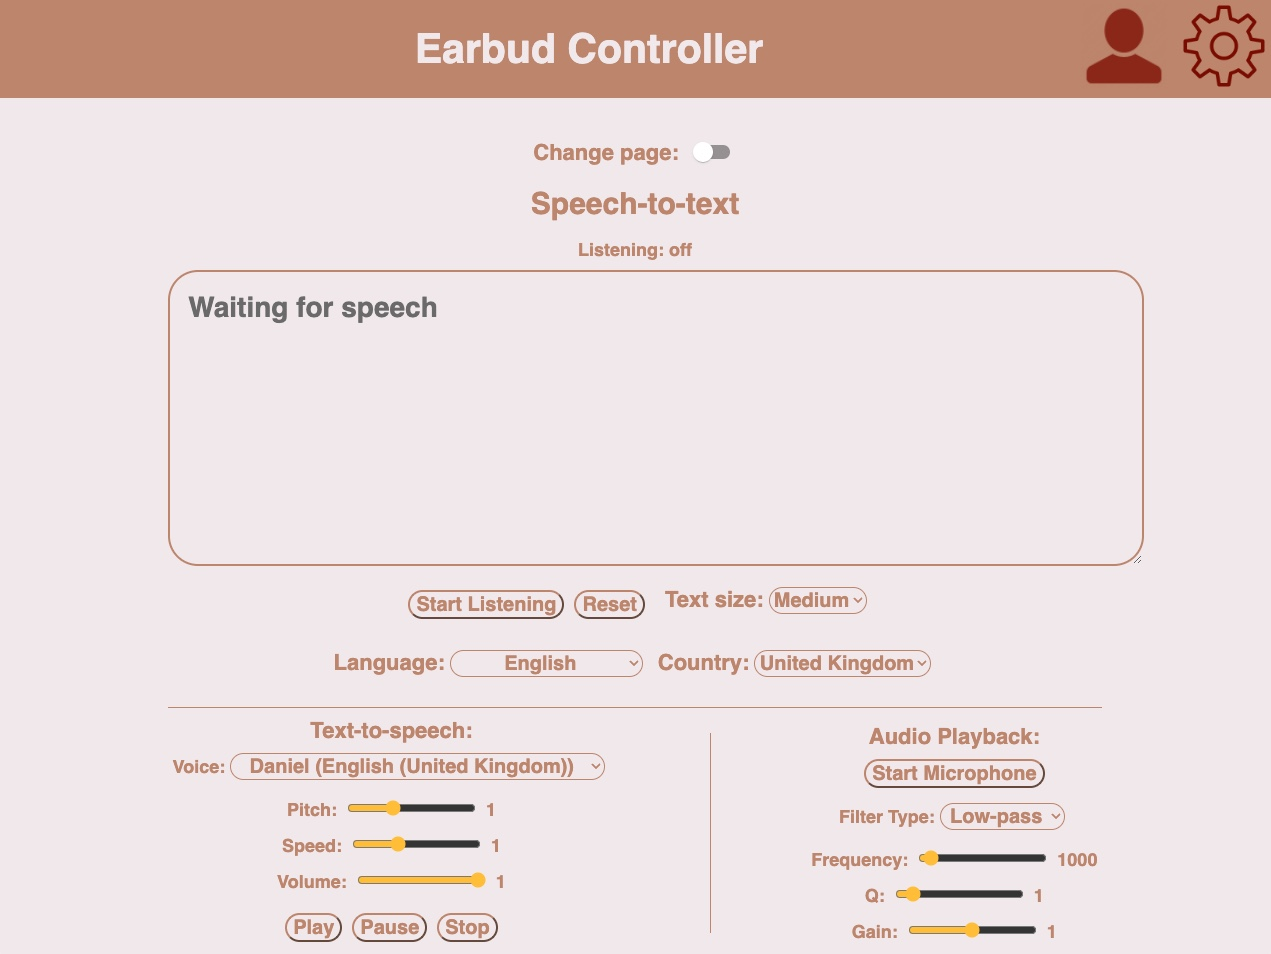
\includegraphics[width=0.85\linewidth]{dissertation/images/captions.jpeg}   
    \caption{This screenshot displays the speech-to-text page of the web-app.}
    \label{fig:captions} 
\end{figure}

\begin{figure}
    \centering
    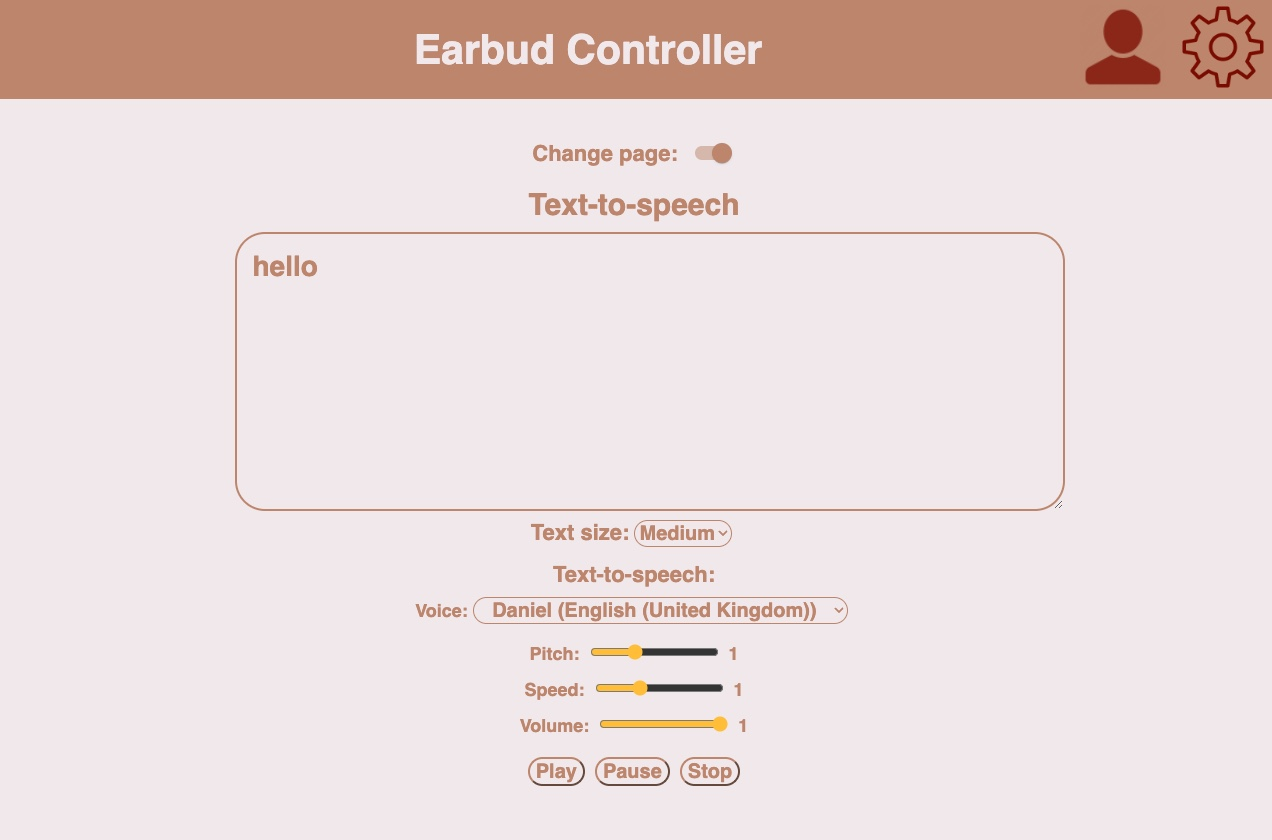
\includegraphics[width=0.85\linewidth]{dissertation/images/text-page.jpeg}   
    \caption{This screenshot displays the text-to-speech page of the web-app.}
    \label{fig:text-page} 
\end{figure}

The Web Speech API seamlessly integrates speech synthesis, facilitating the conversion of text into spoken language. This essential functionality empowers the web application with text-to-speech capabilities, enabling users to receive clear, natural, and customisable auditory feedback, fostering vocal communication. The SpeechSynthesis interface acts as the primary controller for this feature, representing a text-to-speech component that enables programs to articulate their text content. This is achieved through the device's default speech synthesizer. Various voice options are captured by SpeechSynthesisVoice objects, while distinct sections of text designated for speech are encapsulated by SpeechSynthesisUtterance objects. The initiation of spoken output is carried out through the SpeechSynthesis.speak() method. Additionally, the API leverages the speech synthesis systems inherent in most operating systems, ensuring compatibility and optimal performance for this task. These speech recognition interfaces are utilised to create the captions page as seen in Figure \ref{fig:captions}. Along with these screenshots we can see Figure \ref{fig:phone} for each page on a mobile device.

\begin{figure}
    \centering
    \begin{subfigure}[b]{0.30\textwidth}
        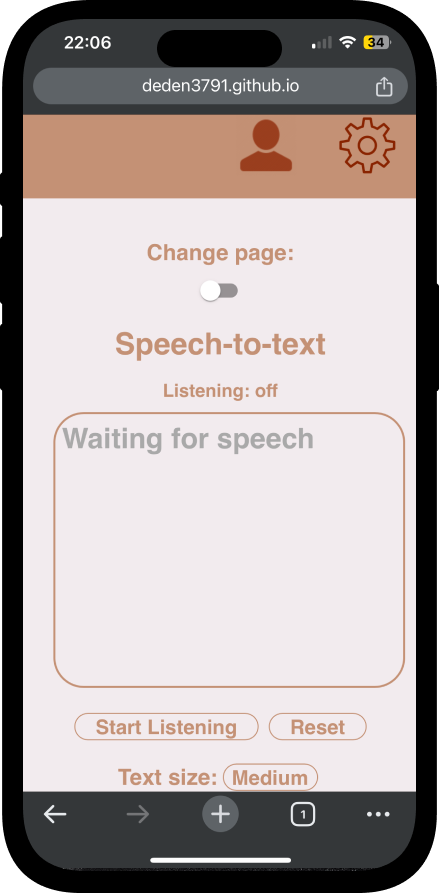
\includegraphics[width=\textwidth]{dissertation/images/captions-phone.png}
        \caption{This screenshot displays the speech-to-text page of the web-app on iPhone.}
        \label{fig:captions-phone}
    \end{subfigure}
    \begin{subfigure}[b]{0.30\textwidth}
        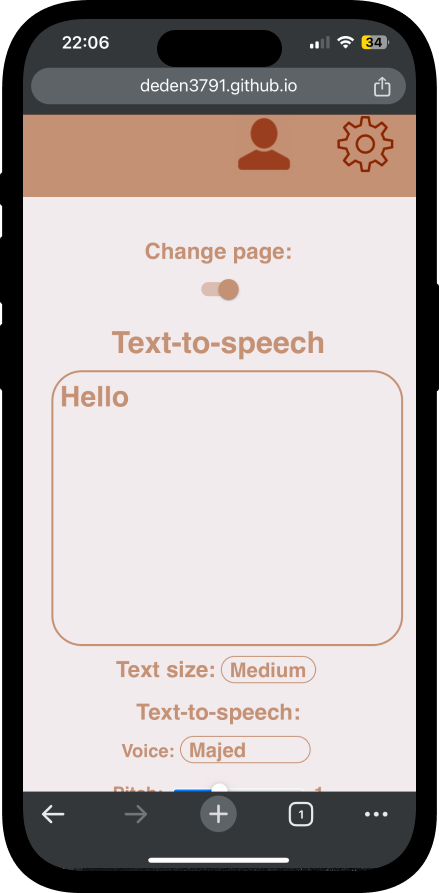
\includegraphics[width=\textwidth]{dissertation/images/text-page-phone.png}
        \caption{This screenshot displays the text-to-speech page of the web-app on iPhone.}
        \label{fig:text-page-phone}
    \end{subfigure}
    \begin{subfigure}[b]{0.30\textwidth}
        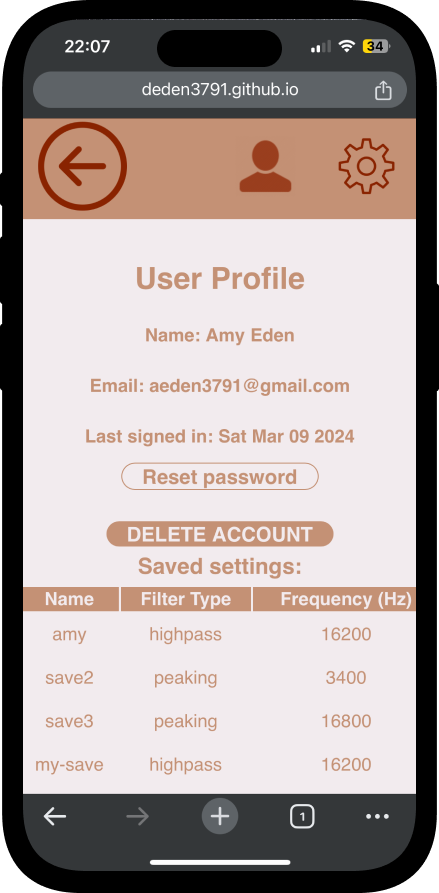
\includegraphics[width=\textwidth]{dissertation/images/profile-phone.png}
        \caption{This screenshot displays the user profile page of the web-app on iPhone.}
        \label{fig:profile-phone}
    \end{subfigure}
    \caption{Displays the web-app on an iPhone to fulfill requirement SH.3 in Section \ref{sec:req}.}
    \label{fig:phone}
\end{figure}

One of the key advantages of leveraging the Web Speech API is its flexibility in customisation. The assistive web application incorporates user preferences for speech recognition and synthesis, allowing individuals to tailor the experience according to their specific needs. This includes adjustments in speech rate, pitch, and language selection utilising Web Audio API. This contributes to a personalised environment for users of all hearing loss to express their identity through communication, to achieve requirement SH.1 aforementioned in Section \ref{sec:req}. This is featured in the text-to-speech page seen in Figure \ref{fig:text-page} along with the speech synthesis methods displayed in Figure \ref{fig:voices}.

Another key advantage of leveraging the Web Speech API is its extensive language support. This feature enables web applications to cater to a diverse audience by providing speech recognition and synthesis capabilities in a wide range of languages to satisfy the SH.5 requirement outlined in \ref{sec:req} as displayed in \ref{fig:languages}. Users can interact with the application using their preferred language, enhancing accessibility and inclusivity to achieve the PA2 outlined in \ref{sec:aims}. This multilingual support expands the reach of the web application to global users, fostering communication and engagement across different linguistic backgrounds, specifically those in countries classified as low- and moddle-income as aforementioned in Section \ref{sec:motivation}. Additionally, the ability to recognise and synthesise speech in various languages contributes to the versatility of the application, making it adaptable to different cultural contexts and user preferences. This comprehensive language support underscores the Web Speech API's efficacy in facilitating effective communication and interaction within web applications.

\begin{figure}
    \centering
    \begin{subfigure}[b]{0.4\textwidth}
        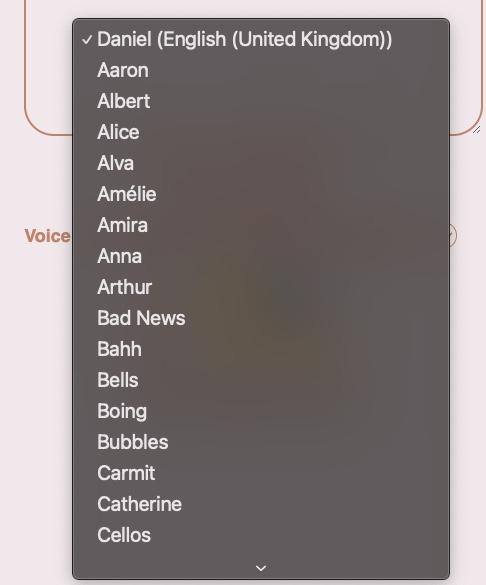
\includegraphics[width=\textwidth]{dissertation/images/voices.jpeg}
        \caption{This screenshot displays just a fraction of the various voices you can choose from for the text-to-speech feature.}
        \label{fig:voices}
    \end{subfigure}
    \begin{subfigure}[b]{0.3\textwidth}
        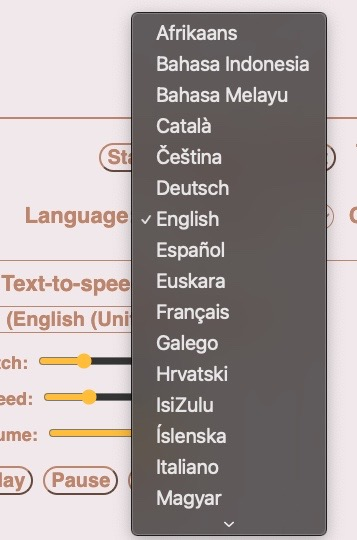
\includegraphics[width=\textwidth]{dissertation/images/languages.jpeg}
        \caption{This screenshot displays the range of languages the web-app supports.}
        \label{fig:languages}
    \end{subfigure}
    \caption{This figure displays the various voices and languages we implemented in the web-app from the Web Speech API.}
    \label{fig:voices-languages} 
\end{figure}

A drawback of utilising this API is its dependency on an internet connection. Throughout this project, we explored a range of technologies, one of which was the Python library called vosk \citep{PyPI}. We initially considered integrating it into the web application. However, the process of integrating Python into React proved to be cumbersome and ultimately not worthwhile due to the significant inaccuracies in the output generated by this method.

\subsection{Web Audio API}
\label{sec:web-audio-API}

The Web Audio API provides developers with a comprehensive toolset for manipulating audio on the web. At its core, it operates within an audio context, where audio operations are orchestrated through a modular routing system. Central to this system are audio nodes, which are interconnected to form an audio routing graph. These nodes represent various audio sources, including oscillators, audio buffers, media elements, and streams \citep{MozDevNet}. 

The audio graph allows for dynamic processing of audio samples, enabling developers to apply effects, modify volume levels, and spatialize audio. Effects nodes, such as reverb, filters, panners, and compressors, can be inserted into the graph to shape the audio according to desired characteristics. This is how we achieved the audio playback requirement (MH.4), outlined in \ref{sec:req}.

Ultimately, the processed audio is routed to a destination, typically the system speakers or headphones, allowing users to hear the audio output. The precise timing and low latency of the Web Audio API enable accurate event response and sample targeting. This capability makes it suitable for applications like drum machines and sequencers, but we are here to test its ability to function as an assistive feature.  Additionally, the API offers spatialization controls, facilitating the placement of audio sources within a virtual environment relative to a listener. This versatile functionality empowers developers to create immersive and interactive audio experiences on the web.

We use the Web Audio API's workflow to create an audio context, which serves as the foundation for all subsequent audio operations. Within this context, various audio sources are instantiated, ranging from elements like <audio> tags to programmatically generated oscillators and streaming audio sources.

Next, we can enhance and manipulate the audio by introducing effects nodes into the audio graph. These nodes, such as reverb, biquad filters, panners, and compressors, allow for a wide range of audio processing possibilities, from spatialization to dynamic tonal shaping. For this context, we are utilising the biquad filters. 

Once the audio has been appropriately modified, we designate the final destination for the audio output, typically the system speakers or headphones. Finally, the sources are connected to the effects nodes, and the effects nodes are connected to the destination, establishing the desired audio flow within the context. This structured approach facilitates the creation of rich and dynamic audio experiences on the web, with precise control over every aspect of the audio signal's journey.

The BiquadFilterNode, established via the createBiquadFilter method within the BaseAudioContext, serves as a pivotal element of the Web Audio API. Functioning as an AudioNode, it embodies various filtering operations, basic tone control, and graphic equalisation. Crucially, each BiquadFilterNode maintains a uniform structure comprising a single input and output, ensuring consistency within audio processing configurations.

With the implementation, users can effortlessly choose from various filter types, as displayed in Figure \ref{fig:filter-type}, using the Web Audio API. The user guide - on the web-app and GitHub - details how each variable influences sound output. Users can email the contact in the user guide to provide any feedback to satisfy the SH.2 requirement aforementioned in Section \ref{sec:req}. In signal processing, these filters serve distinct roles with different relationships to the frequency, Q, and gain values. For example, a low-pass filter allows frequencies below a set cutoff, attenuating higher frequencies, while a high-pass filter does the opposite. The band-pass filter selectively allows a range of frequencies, and a notch filter attenuates a narrow band. Meanwhile, a peaking filter adjusts gain within a specific frequency range. Moreover, there are two more types: the all-pass filter, which allows all frequencies to pass through unchanged but alters their phase relationship, and the notch filter, which attenuates a narrow band of frequencies centered around a specified frequency \citep{MozDevNet_filters}. This versatile toolkit, integrated through the Web Audio API, proves essential for shaping signals in applications like audio processing and telecommunications. See table \ref{tab:filters} for more information.

\begin{figure}
    \centering
    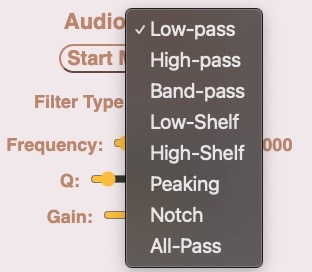
\includegraphics[width=0.4\linewidth]{dissertation/images/filter-type.jpeg}    
    \caption{This screenshot displays the various filter types utilised in the BiquadFilterNode method to provide the audio playback feature.}
    \label{fig:filter-type} 
\end{figure}


\subsection{Clerk}
\label{sec:clerk}

Clerk, an advanced cloud-based authentication service, is specifically tailored for React applications, presenting a comprehensive and developer-friendly solution. Its seamless integration capabilities extend to various front-end frameworks, including React, Next.js, Remix, React Native, and Expo, ensuring broad accessibility within the developer community. Addressing the intricacies of authentication and user management, Clerk boasts a feature-rich environment encompassing user management, organisations, email and SMS authentication, password-less authentication, social login, multi-factor authentication (MFA), multi-sessions, device management, and password leak protection for a save user experience \citep{Grant_2023}. Notably, Clerk distinguishes itself through unique features like Organizations, Multi-Sessions, and Device Management, making it a preferred choice for applications requiring these advanced functionalities.

The React API offered by Clerk significantly enhances developer productivity by providing pre-built components and a hook-based API. These components, including SignIn, SignUp and UserButton, offer ready-made solutions for common authentication tasks such as sign-up, sign-in, and password reset forms \citep{Clerk}. This feature streamlines the development process, reducing the overhead associated with creating custom UI components to upkeep requirement UI.2 outlined in Section \ref{sec:UI}. Moreover, Clerk's React API supports themes, facilitating easy integration with existing website styles, while allowing extensive customization to align with specific design preferences. The combination of user-friendly features, seamless React integration, and robust security measures establishes Clerk as a compelling choice for developers seeking a sophisticated authentication solution for React applications.

In addition to its robust authentication features, Clerk offers a seamless solution for storing and managing saved instances for users, enhancing the overall user experience. Leveraging Clerk's capabilities, developers can implement a secure and efficient system for users to save and select instances as needed within their applications. The versatility of Clerk extends beyond authentication, providing a well-integrated approach to user data storage. By utilising Clerk's functionality, developers can design and implement features that allow users to conveniently save their instances, facilitating a personalized and tailored experience. This capability aligns with Clerk's commitment to providing a comprehensive environment for developers, further solidifying its position as a versatile and sophisticated choice for React applications seeking both authentication and data management solutions.

\begin{figure}
    \centering
    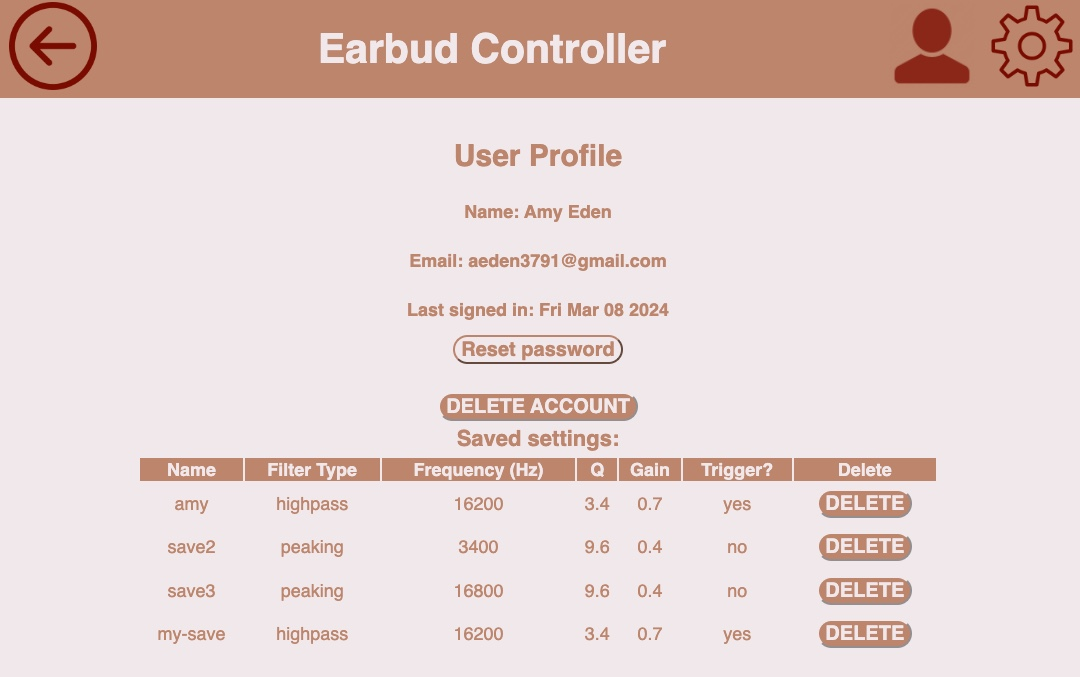
\includegraphics[width=0.9\linewidth]{dissertation/images/profile.jpeg} 
    \caption{This screenshot displays the profile page, including the various save instances for the audio playback feature utilising Clerk.}
    \label{fig:profile} 
\end{figure}

This solution for storing and managing saved instances for users is how we implemented a secure system, enabling users to save and select playback instances for the hearing aid feature within the application. Moreover, users have the ability to assign any saved setting as a trigger word. This functionality allows the speech-to-text feature to automatically switch to the corresponding saved instance when detecting the name associated with it. For instance, if a user has saved an audio instance named 'Amy' for a friend named Amy, and the speech-to-text detects the name 'Amy' (e.g., if the user says "Hello Amy"), the audio playback feature will seamlessly transition to the 'Amy' saved instance.

\begin{figure}
    \centering
    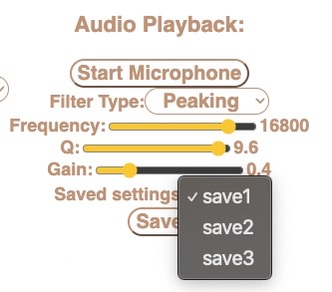
\includegraphics[width=0.4\linewidth]{dissertation/images/saves.jpeg} 
    \caption{This screenshot displays how the playback feature changes, so they can save instances, when the user is logged in utilising Clerk.}
    \label{fig:saves} 
\end{figure}

This versatility extends beyond authentication, aligning with our project's commitment to providing a comprehensive environment for users, solidifying Clerk as a sophisticated choice for our React web-app, addressing both authentication and data management needs. We, also, utilised Clerk to create the user profile page displayed in Figure \ref{fig:profile} with the ability to save audio playback instances displayed in Figure \ref{fig:saves}. These components allowed us to achieve SH.4 outlined in Section \ref{sec:req}.

\chapter{User Study}
\label{sec:user-study}

To delve deeper into the perspectives of the Deaf and Hard of Hearing community regarding assistive technology, I conducted two surveys to fulfill the PA.4 requirement outlined in Section \ref{sec:aims}. The first survey aimed to gather insights into individuals' expenditure on assistive technology, their satisfaction levels with existing solutions, and introduced our project, inviting feedback on desired features and improvements. The second survey focused on assessing the overall usability of assistive technology, extending the evaluation to include the System Usability Scale (SUS) \citep{SUS}. 

To calculate SUS, prompts with positive connotations contribute to the score by subtracting one from the scale position, while prompts with negative connotations contribute by subtracting the scale position from 5. The sum of these scores is then multiplied by 2.5 to determine the overall value of SUS. Typically, the scale ranges from 0 to 100, but we included additional questions related to the project, which ranges from 0 to 150. We ensured to calculate the official System Usability Scale (SUS) using only the 10 questions outlined in the paper; as well as our modified version.

Throughout the engagement with the Deaf and Hard of Hearing community, it became evident that there's a prevailing sentiment of fatigue with researchers constantly approaching them for surveys. Many expressed feeling as through they are treated as exhibits in a zoo, where researchers come in, conduct surveys, and leave without meaningful engagement or follow-up. It's crucial to acknowledge and respect these sentiments, recognising that Deaf individuals are not mere subjects for research but individuals with their own agency and perspectives. Referring to the outlined project aim PA.3 in Section \ref{sec:aims} we must take this perspective into consideration and question if this project is even needed in this society.

\section{Affordability and Satisfaction of Assistive Technology}
\label{sec:afford-survey}

This survey aims to gather information on Deaf and Hard-of-Hearing individuals' experiences with assistive technology, their satisfaction levels with these technologies, and to introduce the new assistive web-app.

The survey received 47 responses, predominantly comprising individuals aged between 45 and 64. This reflects a notable demographic skew towards an older population. This demographic trend suggests a focus on the needs and preferences of older individuals regarding assistive technologies. Particularly within the scope of the user interface and experience (UI/UX) of the web-app, as aforementioned in Section \ref{sec:design}. Furthermore, the survey indicates a prevalent degree of hearing loss among respondents, with a substantial 66\% experiencing moderate hearing loss.

The survey reveals a widespread reliance on assistive technologies among respondents, with nearly half utilising hearing aids. Despite this widespread adoption, satisfaction levels vary across different assistive technologies. Notably, while the satisfaction levels within hearing aids are spread out, a majority expressed high satisfaction with hearing aids. These satisfaction levels drop, with a majority reported significantly less satisfaction with speech-to-text capabilities, and even less satisfaction with text-to-speech capabilities.

A noteworthy finding from the survey pertains to the funding status of assistive technologies, with a slight majority of respondents receiving funding support. However, satisfaction levels differ between funded and non-funded individuals, with funded users expressing higher levels of satisfaction. Interestingly, while a considerable portion of respondents spend nothing on assistive technology, those who do report spending over £1,000 exhibit varying levels of satisfaction.

The survey delves into the diverse expectations of assistive technologies by users, including clear sound quality, accurate speech-to-text capabilities, ease of use, and customisation options. Respondents also express preferences for discounted pricing, long battery life, and compatibility with other devices. However, concerns regarding privacy, data security, and the effectiveness of proposed products in noisy environments are also apparent. 

While approximately 28\% of respondents found the proposed product useful, various suggestions and apprehensions highlight the importance of addressing user concerns and preferences in the development of assistive technologies. For instance, a participant proposed a feature for the web-app, suggesting the incorporation of an arrow indicating the direction from which sounds, and consequently speech, emanate. This would aid the user in identifying the speaker. Due to the project's defined scope, this feature was not implemented. However, it warrants consideration for future iterations of the web-app.

In conclusion, these findings emphasise the complex interplay between funding, costs, and user satisfaction in the adoption and utilisation of assistive technologies among individuals with hearing loss. These findings underscore the importance of user-centric design, cost considerations, and compatibility with existing technologies in the development and implementation of assistive solutions. By addressing user needs and concerns, developers and policymakers can ensure the development of more effective and inclusive assistive technologies to enhance the quality of life for individuals with hearing loss.

\section{Usability of Assistive Technology}
\label{sec:use-survey}

This survey aims to gather information on individuals' thoughts on the usability of assistive technology by analysing both quantitative and qualitative data. 

The survey garnered 24 responses, with the majority of participants being in the 35-44 age range, providing a broad perspective on the topic. A significant portion of participants reported profound hearing loss, highlighting the prevalence of severe impairment within the surveyed population. The average, modified System Usability Scale (SUS) score of 81.04, alongside an official SUS score of 59.69, indicates generally positive usability experiences with assistive technologies, suggesting room for improvement in specific areas. This data is visualised in Figure \ref{fig:survey-SUS}.

\begin{figure}
    \centering
    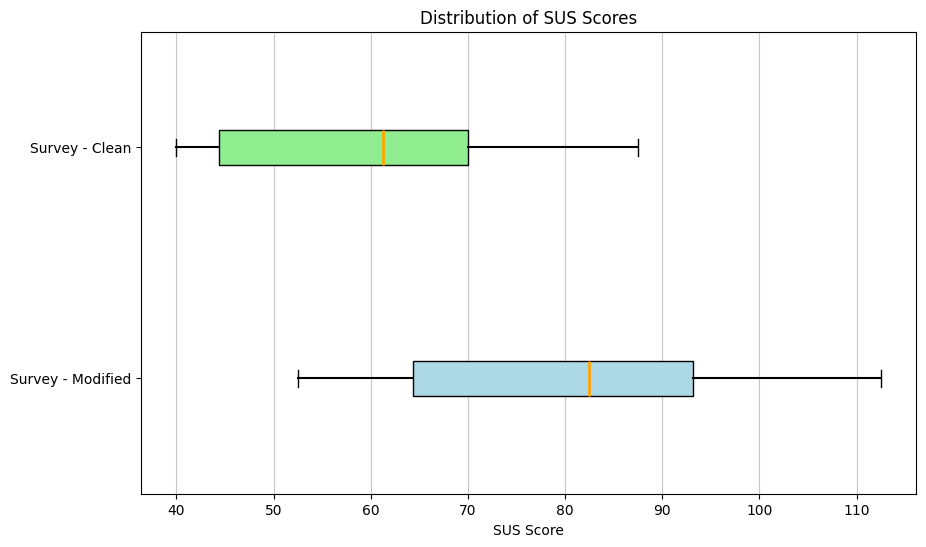
\includegraphics[width=0.9\linewidth]{dissertation/images/SUSSurvey.png}    
    \caption{This figure compares responses to 10 original questions with those to 2 additional questions probing perspectives on current assistive technology solutions.}
    \label{fig:survey-SUS} 
\end{figure}

During the qualitative analysis, we found that many respondents expressed frustration with phone communication due to inaccurate transcription apps and unreliable transcribing services during calls. This poses significant obstacles in both professional and social interactions. This is why we tested the speech-to-text feature during a phone call, and it effectively transcribed the conversation.

Issues with hearing aid functionality were also highlighted, including vulnerability to moisture, intrusive sound dampening features, and limitations in streaming capabilities. However, there were positive experiences shared regarding the effectiveness of assistive technology in empowering Deaf children, fostering independence, and facilitating educational and social development.

Despite advancements, current assistive technologies still face limitations, including reliance on Wi-Fi connectivity, challenges in noisy environments, and the need for a holistic communication approach beyond technology alone. Some respondents also highlighted the financial burden associated with acquiring assistive devices, emphasising the need for better accessibility and support programs to alleviate costs, which this project aims to do.

Additionally, respondents emphasised the significance of accommodating Deaf individuals' language preferences and recognising the limitations of spoken language-centric technologies. This is because the Deaf community does view English as their second language \citep{Morgan_2016}, with sign language being their first. One respondent articulated this sentiment by questioning why Deaf individuals should be expected to communicate in a second language, while hearing individuals often neglect to learn Deaf individual's first language. They challenged assumptions about Deaf people's desire to communicate in English and questioned the underlying assumption that solutions are needed to fix perceived problems. Instead, they highlighted that technology should serve to facilitate communication between hearing and Deaf individuals, rather than aiming to fix Deaf individuals themselves as a cultural model. This perspective sheds light on the concept of audism and underscores the importance of understanding and respecting Deaf culture and language.

In summary, while there are positive aspects to current assistive technologies, there remain significant challenges and areas for improvement in usability, communication options, financial accessibility, and design considerations to better meet the diverse needs of users with hearing loss.


%==================================================================================================================================
\chapter{Evaluation} 
\label{sec:evaluation}

The aim of this project, as outlined in \ref{sec:aims}, is to evaluate a proof of concept for an affordable solution tailored to the needs of the Deaf and Hard-of-Hearing (DHH) community, leveraging the Web Speech API. By incorporating features described in Section \ref{sec:req}, the web application aims to foster inclusivity for individuals with various types of hearing loss. The primary objective is to provide cost-effective accessibility solutions while accommodating the diverse needs of the DHH community for the web-app to be usable. Furthermore, the project endeavours to create an open-source platform, enabling ongoing development and improvement beyond my own dissertation.

Evaluating assistive technology (AT) involves assessing the extent to which ATs effectively enhance participation, address loss, and alleviate health-related limitations. In essence, it entails gauging the overall effectiveness and usefulness of assistive technologies \citep{tao2020evaluation}. This is why we chose to employ the System Usability Scale (SUS) \citep{SUS}, as we used in Section \ref{sec:user-study} to evaluate if requirement PA.4 outlined in Section \ref{sec:aims} has been achieved. Furthermore, leveraging the findings from the analysis conducted in Section \ref{sec:user-study}, we will undertake a comparative evaluation of the usability between the existing assistive technology and the newly introduced assistive web application. To evaluate the requirements outlined in Sections \ref{sec:UI} and \ref{sec:UX}, we expanded upon the original 10 System Usability Scale (SUS) statements, creating 17 statements while adhering to the same scoring methodology (i.e., subtracting one for positive statements and subtracting the score from 5 for negative statements). We will analyse the original SUS score along with our modified version. In addition to te quantitative analysis, we also utilise the qualitative data for a deeper analysis.

The assessment was distributed to individuals with and without hearing loss to complete 8 sections. Hearing individuals are encouraged to use noise-canceling earbuds or headphones, when testing the web-app. This is intended to provide a modest simulation to assess the effectiveness of the web-app.

\section{Overview}

First, we encouraged each participant to familiarise themselves with the web-app's interface before proceeding to the five sections, each containing a distinct task outlined in the provided user guide \footnote{\url{https://github.com/deden3791/L4Project/blob/main/main/UserGuides/UserGuide.md}}. Upon completion of each task, the participant is kindly asked to answer questions sharing their experience and feelings regarding the utilisation of the feature.

The evaluation intends to assess each feature against qualities such as being:

\begin{itemize}
    \item Intuitive: does each feature feel intuitive?
    \item Accurate: does each feature perform accurately?
    \item Comfortable: does each feature feel comfortable to use?
    \item Usable: is each feature usable?
\end{itemize}

The evaluation received 17 responses, with  Figures \ref{fig:ages} and \ref{fig:hearing} illustrating the distribution of ages and hearing loss among our participants. When analysing both the quantitative and qualitative data of the responses, we meticulously distinguish between the perspectives of the hearing and the Deaf and Hard-of-Hearing community.

\begin{figure}
    \centering
    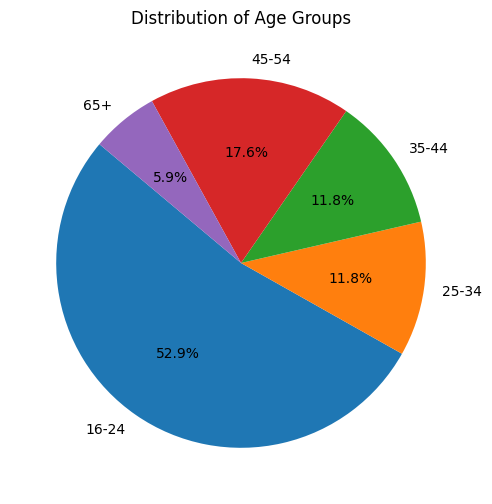
\includegraphics[width=0.6\textwidth]{dissertation/images/ages.png}
    \caption{This pie chart displays the age distribution of participants.}
    \label{fig:ages}
\end{figure}

\begin{figure}
    \centering
    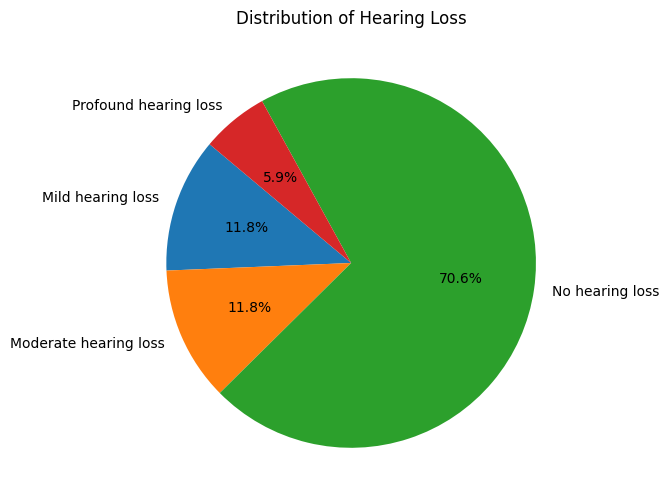
\includegraphics[width=0.7\textwidth]{dissertation/images/hearing.png}
    \caption{This pie chart displays the hearing distribution of participants.}
    \label{fig:hearing}
\end{figure}

For each task, we utilised a Likert scale ranging from 'Strongly Agree' to 'Strongly Disagree'. However, we recognise the inherent challenges in analysing Likert scales \citep{harpe2015analyze, likert}. To address this, we convert the responses into numerical values and standardise them on a 0-4 scale, similar to how we handle the System Usability Scale (SUS). This approach helps mitigate common pitfalls associated with Likert scale interpretation.

\section{Speech-to-text Feedback}

For this task, the participants were asked to navigate to the speech-to-text section. They were then asked to select their preferred language and region. Once they were comfortable they were prompted to click the "Start Listening" button to initiate the conversation to engage in verbal communication as desired. Once the conversation had finished, they were to click the "Stop Listening" button to conclude the web-app's listening mode.

Both hearing and non-hearing participants unanimously agreed that the speech-to-text feature felt intuitive, accurate, and comfortable, with the lowest average being 3.2 as seen in Figure \ref{fig:STT-chart} However, some participants pointed out certain limitations, such as the feature's occasional failure to recognise acronyms like 'LOL', often mistaking them for 'Hello'. Additionally, one participant reported compatibility issues with the 'Ark' browser, attributed to restrictions within the Web Speech API that render it suitable for specific browsers. Furthermore, a few participants observed minor inaccuracies in the transcription, attributing them to their strong Yorkshire accent. The persistent challenge posed by accent variations in speech recognition systems is a notable issue, as discussed in Section \ref{sec:speech-recog}, warranting further attention and awareness.

\begin{figure}
    \centering
    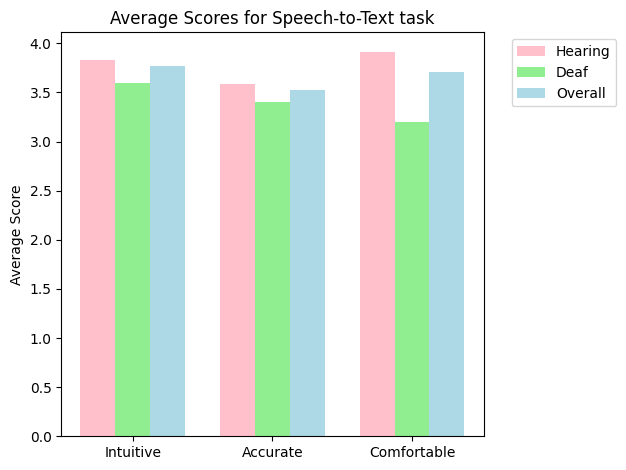
\includegraphics[width=0.6\textwidth]{dissertation/images/STT.png}
    \caption{This bar chart displays the scores for the Speech-to-Text task on a 0-4 scale.}
    \label{fig:STT-chart}
\end{figure}

\section{Speech-to-text with Text-to-speech Feedback}

For this task, participants are instructed to begin by using earbuds or headphones. They then proceed to access the speech-to-text feature as outlined in the previous task. Following this, they have the option to click the "Play" button on the text-to-speech feature to listen to the converted text. Additionally, participants are encouraged to modify the settings within each feature, such as languages for speech-to-text and speed, pitch, volume, and voice for text-to-speech. They can also pause or stop the speech-to-text and text-to-speech features as necessary during their interaction.

For hearing participants, the speech-to-text feature, along with the text-to-speech feature, was unanimously perceived as intuitive, with a rating of 3.9 as seen in Figure \ref{fig:STT-TTS-chart}. However, we do see a 0.9 drop in the rating for our Deaf and Hard-of-Hearing participants. It is important to note that, there is a 0.5 drop in hearing participants finding the feature accurate and comfortable to use. This may be due to them experiencing no hearing loss so these features are not comfortable for them to use. For Deaf and Hard-of-Hearing individuals, the rating for accuracy and comfortability raised by 0.2. 

Several participants noted that the accuracy of the speech-to-text feature varied significantly depending on the microphone used. For example, they found it more accurate when using headphones connected via wire or when using the laptop's built-in microphone instead of headphones. Others expressed frustration with default settings, mentioning that their devices would revert to default settings, requiring them to change language or voice settings repeatedly, which they found cumbersome. Additionally, some participants found the text-to-speech output to be choppy and unnatural, lacking the fluidity of a normal conversation. This aspect of speech synthesis is an ongoing area of improvement, as discussed in Section \ref{sec:speech-syn}, and warrants further attention. 

\begin{figure}
    \centering
    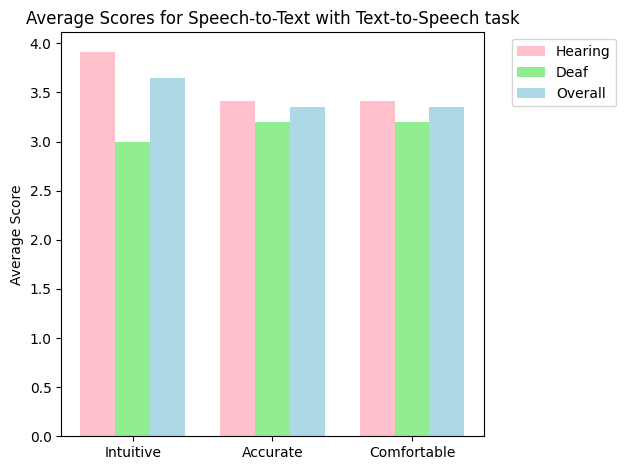
\includegraphics[width=0.6\textwidth]{dissertation/images/STT-TTS.png}
    \caption{This bar chart displays the scores for the Speech-to-Text with Text-to-Speech task on a 0-4 scale.}
    \label{fig:STT-TTS-chart}
\end{figure}

\section{Audio Playback Feedback}

For this task, participants were instructed to start by using earbuds or headphones for optimal audio experience. Next, they were guided to navigate to the audio playback section and encouraged to familiarise themselves with the available adjustable variables. Participants were informed that they could access additional details by referring to the settings icon in the header. Once participants felt comfortable with their chosen settings, they were prompted to click the "Start Microphone" button to initiate the conversation. Additionally, participants were reminded of their flexibility to modify settings at any point during the interaction.

Hearing participants appeared to perceive the feature as intuitive, evidenced by a 3.4 rating as depicted in Figure \ref{fig:PB-chart}. This rating slightly decreased by 0.4 for Deaf and Hard-of-Hearing participants. Nevertheless, all Deaf and Hard-of-Hearing participants unanimously considered the feature both accurate and comfortable, averaging a rating of 3.4. In contrast, hearing participants rated the accuracy slightly higher at 3.6, while their comfort rating was slightly lower at 3.3. Again, this discomfort experienced by some hearing participants could be attributed to their unaffected hearing capabilities, leading them to perceive the feature as uncomfortable due to its alteration of their finely tuned auditory experience. This contrasts the aid that this feature may give a Deaf user. 

Some participants expressed confusion regarding the functionality of each variable in altering the surrounding sound, indicating a need for more emphasis on the user guide. Suggestions were made, including implementing pop-ups when hovering over the variables to provide clearer explanations. Additionally, although the abundance of variables was acknowledged as beneficial for usability, it was also noted that they could potentially overwhelm users and lead to feature abandonment. We acknowledge the significant abandonment rate associated with assistive technologies \citep{ijerph18147259}. Therefore, we have enhanced our user guide to provide greater clarity and understanding, aiming to mitigate this issue.

One participant highlighted the necessity for significant layout improvements within the web-app to be able to distinguish features with ease. They specifically noted the need for increased spacing between elements, noting frustration when using the web-app on a mobile devices due to oversized finger interactions with sliders. In response, we implemented borders between each feature and increased spacing between variables to address these usability concerns effectively.

\begin{figure}
    \centering
    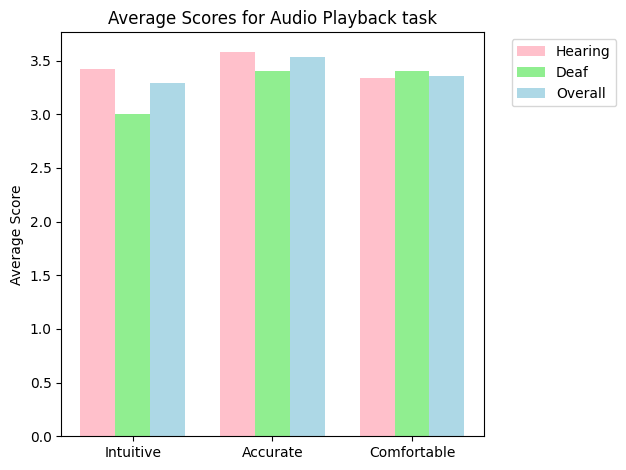
\includegraphics[width=0.6\textwidth]{dissertation/images/PB.png}
    \caption{This bar chart displays the scores for the Audio Playback task on a 0-4 scale.}
    \label{fig:PB-chart}
\end{figure}

\section{Creating an Account \& Saving Audio Playback Instances Feedback}

For this task, participants were directed to register by creating an account and explore the functionality of saving audio playback instances. They were instructed to click the account icon in the header and enter the required information for registration. After successfully creating their account, participants were prompted to navigate to the audio playback section. Here, they were encouraged to familiarise themselves with the options available for saving instances and experiment with any customisation features offered (i.e. changing the audio playback variables, saving this audio instance, and even making the save name a trigger word). If participants desired to delete any instances, they were instructed to access their user profile page using the account icon.

All hearing participants unanimously agreed that both the features and save instances felt intuitive and comfortable, with both aspects receiving an approximate rating of 3.8 as depicted in Figure \ref{fig:ACC-chart}. However, when it came to account creation, the rating for intuitiveness decreased by approximately 0.3. In contrast, for Deaf and Hard-of-Hearing participants, these ratings were notably lower, with account creation being perceived as intuitive at 2.8. Similarly, for save instances, only 3.0 found them intuitive. Comfort ratings were also lower among Deaf and Hard-of-Hearing participants, with a rating of 2.8. One participant noted that having the save button change colour when it is a saved setting might inform the user that a change has been made. 

Despite many positive responses regarding the trigger word feature for naming saves, it was observed that the accuracy of save names depended heavily on how the speech recognition system formatted words. For instance, one participant named a save "passthrough", but the system outputted the text as "pass through," leading to the trigger word not being detected. 

\begin{figure}
    \centering
    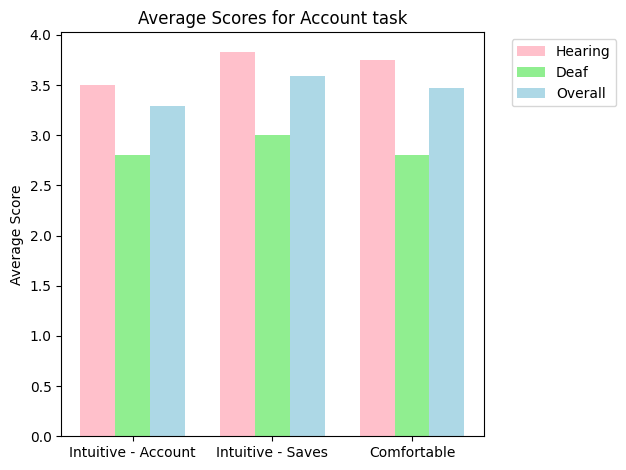
\includegraphics[width=0.6\textwidth]{dissertation/images/ACC.png}
    \caption{This bar chart displays the scores for the Account task on a 0-4 scale.}
    \label{fig:ACC-chart}
\end{figure}

\section{Text-to-speech Feedback}

In this task, participants were guided to explore another feature within the application by clicking the toggle button to access another, separate text-to-speech functionality. They were instructed to enter a set of text or sentences into the designated input field and ensure they were comfortable with the content. Subsequently, participants were prompted to activate the text-to-speech function by clicking the "Play" button and attentively listen to the synthesised speech output. They were encouraged to assess various aspects such as speech clarity, intonation, and overall satisfaction with the text-to-speech functionality.

All hearing participants unanimously expressed strong agreement that the text-to-speech feature felt intuitive, garnering a maximum rating of 4.0. Additionally, they concurred that the feature felt natural and comfortable, receiving a commendable rating of 3.7 and 3.8 respectively. However, among Deaf and Hard-of-Hearing participants, we observed lower ratings for the perceived intuitiveness, accuracy, and naturalness of the feature, all averaging at 3.4.

Participants expressed the necessity of a save configuration option for the text-to-speech feature, as implemented for the playback feature. Additionally, some participants emphasised the need for a testing feature, enabling users to input a phrase for the system to repeat, facilitating adjustment of sliders for optimal settings. Along with these suggestions, participants reiterated their dissatisfaction with the choppiness of the voices. 

\begin{figure}
    \centering
    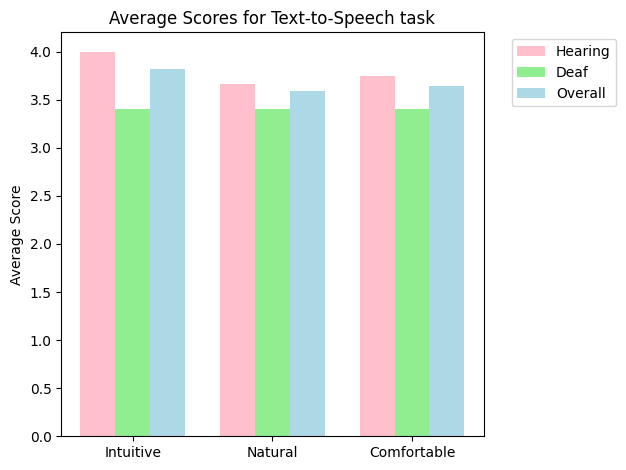
\includegraphics[width=0.6\textwidth]{dissertation/images/TTS.png}
    \caption{This bar chart displays the scores for the Text-to-Speech task on a 0-4 scale.}
    \label{fig:TTS-chart}
\end{figure}

\section{Usability Feedback}

As mentioned in Section \ref{sec:evaluation}, we modify the SUS to analyse if this web-app satisfies our project aims outlined in Section \ref{sec:aims}. Figure \ref{fig:eval} shows the distribution of modified SUS scores to assess the PA.4 project aim, separated into hearing and Deaf and Hard-of-Hearing individuals. For our Deaf and Hard-of-Hearing participants, we calculated an average, modified SUS score of 94.4 out of a potential 170, with a higher 132.5 from our hearing participants. 

\begin{figure}
    \centering
    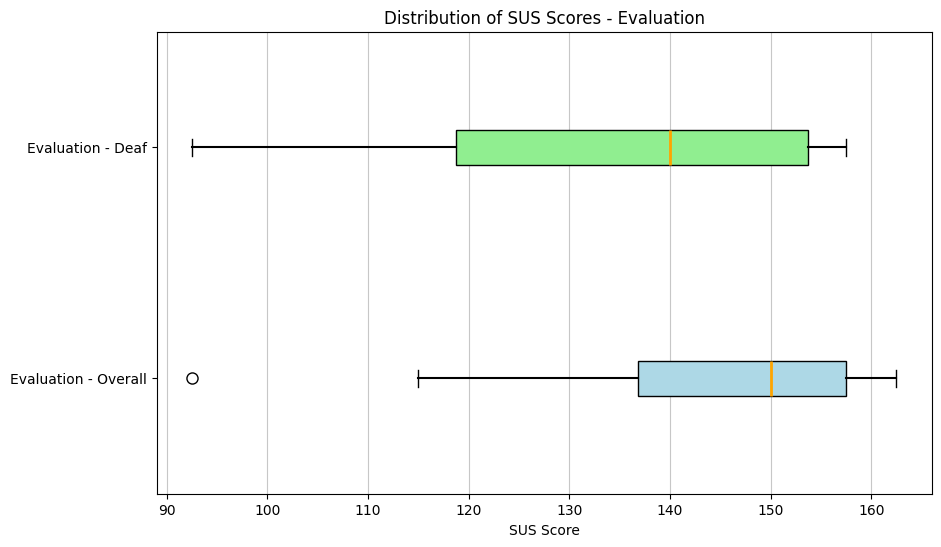
\includegraphics[width=0.75\linewidth]{dissertation/images/EvaluationBoxPlots.png}    
    \caption{This shows the modified SUS scores for the evaluation, separated into hearing and Deaf and Hard-of-Hearing participants, that range from 0 to 170.}
    \label{fig:eval} 
\end{figure}

\begin{figure}
    \centering
    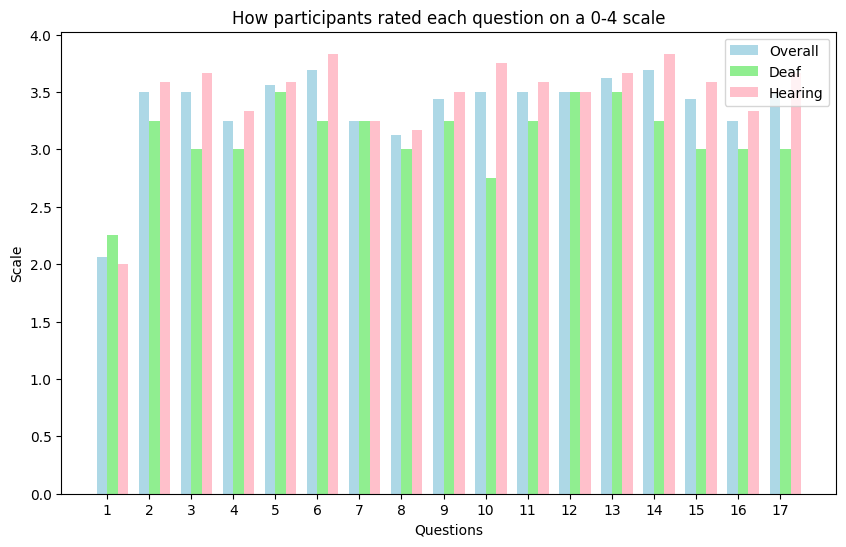
\includegraphics[width=0.75\linewidth]{dissertation/images/questions.png}    
    \caption{This shows the scores of each statement, separated into overall, hearing, and Deaf and Hard-of-Hearing participants, that range from 0 to 4.}
    \label{fig:questions}
\end{figure}


To assess whether the outlined requirements have been fulfilled, we employ a scoring system similar to the calculate of the System Usability Scale (SUS), ranging from 0 to 4. For a detailed mapping of questions to requirements, please refer tables \ref{tab:UI-table} and \ref{tab:UX-table}. For an outline of the scores for overall, hearing and Deaf participants, please refer to Figure \ref{fig:questions}. When analysing the scores given by hearing participants and Deaf and Hard-of-Hearing participants, we calculated a standard deviation of 0.3. While this may not be considered exceptionally large, it should still be deemed significant when justifying if this web-app will be effective to the Deaf and Hard-of-Hearing community.

% \begin{figure}
%     \centering
%     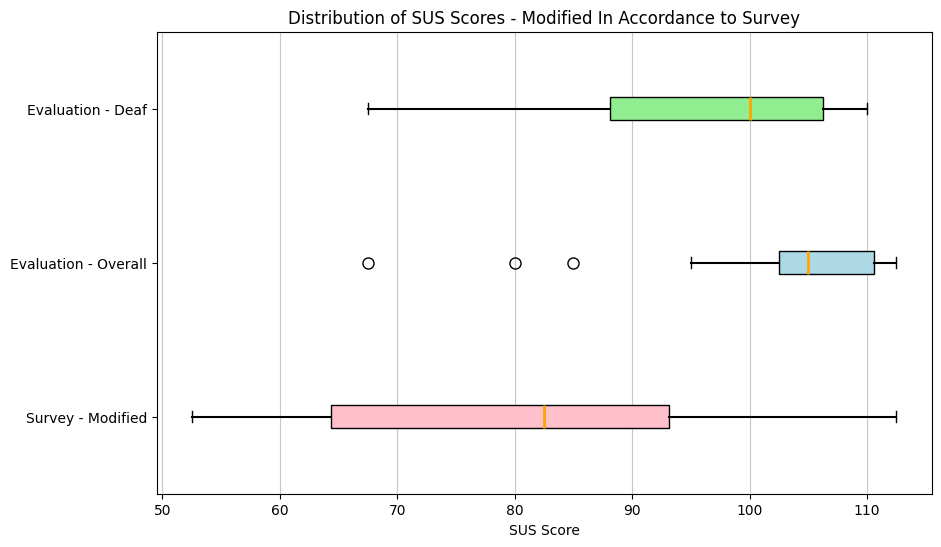
\includegraphics[width=0.75\linewidth]{dissertation/images/ComparisonSurvey.png}    
%     \caption{}
%     \label{fig:comp-survey} 
% \end{figure}

As previously stated, each of the requirements outlined in Sections \ref{sec:UI} and \ref{sec:UX} is associated with the statements given in the evaluation. To analyse if these requirements were fulfilled, we took the average score for each statement and averaged the statements associated with that requirement, as shown in Figure \ref{fig:requirements}. The average deviation between hearing and Deaf and Hard-of-Hearing participants is calculated as 0.4, with a maximum deviation of 1. Again, while this deviation may not be considered exceptionally large, it should still be deemed significant when justifying if these requirements are fulfilled.

Upon examining the individual requirements, we found that each received a rating equal to or greater than 2.75, with an average of 3.12 and a standard deviation of 0.2, indicating that all requirements were met to some extent. Notably, requirements UX.6 and UI.6, which pertain to error communication and user guides, respectively, emerged as areas in need of enhancement. Some participants encountered difficulties with the user guide, prompting us to revise it to provide clearer explanations of the system, thereby fostering better user understanding. The requirement with the highest rating was UI.2, reflecting the web-app's consistency. This positive feedback underscores the effectiveness of maintaining uniformity throughout the user interface, contributing to a smoother user experience.

After removing our additional 7 statements and including only the original 10 SUS statements, we calculated an average SUS score of 75.6 from our hearing participants, with a slightly lower average SUS score of 70 from our Deaf and Hard-of-Hearing participants. Although this deviation of 5.6 isn't notably large, it does signify some areas for improvement in the web-app.

\begin{figure}
    \centering
    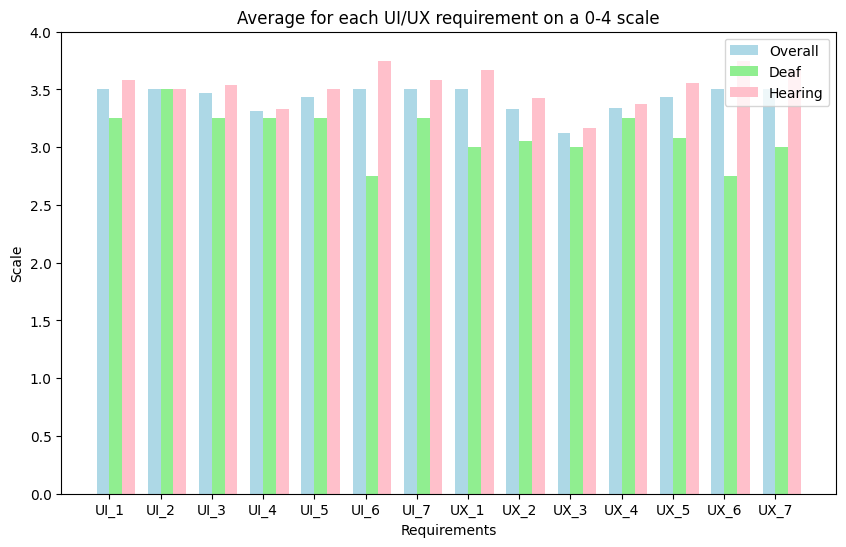
\includegraphics[width=0.75\linewidth]{dissertation/images/requirements.png}    
    \caption{This shows the average scores of each requirement, separated into overall, hearing, and Deaf and Hard-of-Hearing participants, that range from 0 to 4.}
    \label{fig:requirements}
\end{figure}

% \begin{figure}
%     \centering
%     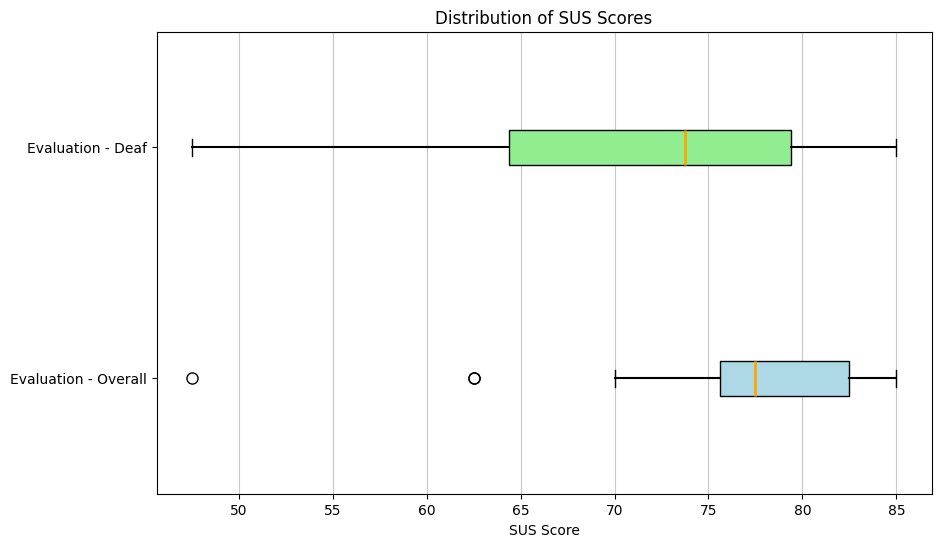
\includegraphics[width=0.75\linewidth]{dissertation/images/ActualSUSEval.png}    
%     \caption{}
%     \label{fig:eval-SUS} 
% \end{figure}

When comparing the SUS scores obtained in this evaluation to those obtained from the survey outlined in Section \ref{sec:user-study}, a remarkable increase in scores is evident. In the survey, the SUS score obtained was 59.69, significantly lower than the score of 70 obtained from our Deaf and Hard-of-Hearing participants, as illustrated in Figure \ref{fig:comp-SUS}. This data strongly suggests that our web-app exhibits greater usability compared to the current assistive technologies utilised by the Deaf and Hard-of-Hearing community. 

\begin{figure}
    \centering
    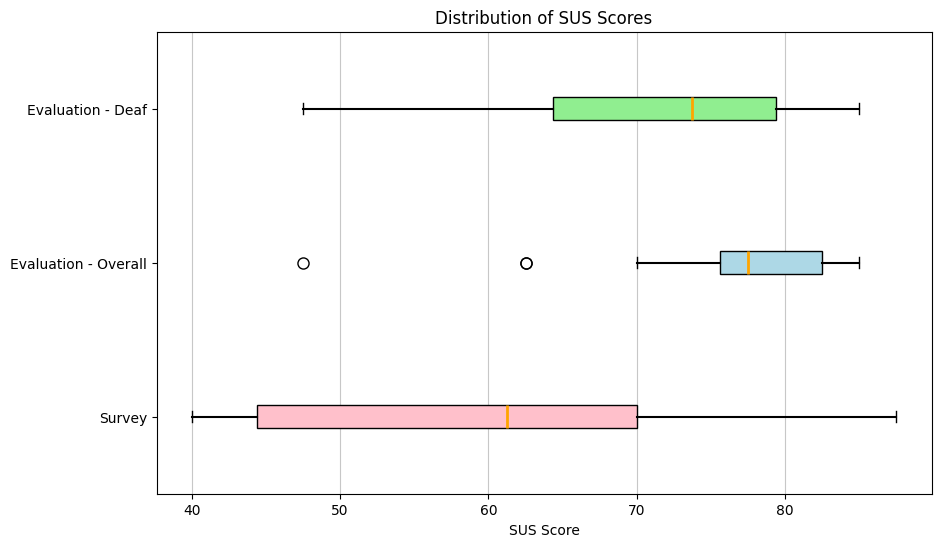
\includegraphics[width=0.75\linewidth]{dissertation/images/ActualSUS.png}    
    \caption{This shows the official SUS scores comparing the overall, Deaf and Hard-of-Hearing, and survey scores.}
    \label{fig:comp-SUS} 
\end{figure}

\section{Limitations}

While the evaluation provides valuable insights into the web-app's usability, many limitations should be considered when interpreting the results and making decisions based on them. For example, the evaluation's sample size of 17 participants is notably small, particularly with only 5 participants representing the Deaf and Hard-of-Hearing community. This limited representation may not capture the full spectrum of experiences and preferences within this user group, potentially impacting the ability to generalise the findings. Furthermore, it's important to note that several participants in the evaluation are family and friends, which could introduce bias into the results. Participants with personal connections to the developers or project team may provide feedback influenced by loyalty or familiarity, rather than unbiased assessments of usability.

Although efforts were made to simulate real-world scenarios and encourage natural interactions during the evaluation, the controlled nature of the study may still limit its applicability to diverse usage contexts. Individual preferences, prior experiences, and environmental factors can significantly influence usability in real-world settings, and these nuances may not have been fully captured in the evaluation. Efforts were made to recruit participants from diverse backgrounds by posting the evaluation on many Deaf and Hard-of-Hearing online groups, though the small sample size remains a constraint to keep in mind Expanding the participant pool to include a more diverse range of users, particularly from the target demographic of Deaf and Hard-of-Hearing individuals, would strengthen the validity and make it easier to generalise the findings.

%==================================================================================================================================
\chapter{Conclusion}
\label{sec:conclusion}

This project was motivated by the gap in affordable assistive technology within the Deaf and Hard-of-Hearing community that legislation such as the United Nations Convention on the Rights of Persons with Disabilities (CRPD) \citep{United_Nations} fails to bridge \citep{00006479-201135010-00003}. Bridging this gap is specifically important due to the cost-of-living crisis \citep{broadbent2023public}, impacts of quality of life without assistive technology \citep{borre2023impact, ijerph18147259}, with detrimental links to dementia \citep{dementia, 10.1001/archneurol.2010.362, livingston2020dementia, loughrey2018association} and mortality \citep{choi2024association}.

Before deep-diving into developing assistive technology, it is important to understand Deaf culture throughout history to know what kind of assistive technology you develop: through cultural perspective or an infirmity model \citep{burrows2022not}. From the rudimentary ear-trumpets constructed from skeletal remains \citep{CalHearing_2023} to the current development of programmable multi-modal hearing aids \citep{shah2022novel}, assistive technology has undergone rapid evolution. However, alongside these advancements, the associated costs have also escalated \citep{Market_Research_Firm}.

Throughout this project, we define many requirements to be fulfilled utilising Web Speech API to prove that low cost assistive technology can be made. The evaluation results show a usability rating of 70 out of a possible 100 from the Deaf and Hard-of-Hearing community. Alongside this, the requirements we outlined received an average rating of 3.12. This proves that the web-app fulfilled the requirements with room for improvement. 

Future work could entail focusing on the initial plan of the project for real-time amplification and edge-computing. In relation to the current project, it is worthwhile delving deeper into speech recognition, particularly in terms of accent variability \citep{Lopez-Lloreda_2020, koenecke2020racial}. This emerged as a notable challenge during the evaluation process. Additionally, there is a need to explore complex features outlined in requirement WH.2 in Section \ref{sec:aims}, such as speaker detection, siren detection, and offline capabilities, which were not fully implemented in this project. Although some progress was made towards speaker detection, no concrete feature was developed. However, this functionality holds promise as a foundational element for real-time captioning systems aimed at distinguishing between speakers. Moreover, as discussed in Section \ref{sec:user-study}, an intriguing potential enhancement involves speaker detection leveraging directional sound cues. This feature would visually represent the speaker's orientation on the screen, potentially through an arrow indicator. Such advancements could significantly enhance the accessibility and usability of the web-app for users with diverse needs.

Although this project did delve into the Deaf and Hard-of-Hearing community for their opinions and guidance on assistive technology, it is important to note that this web-app is an infirmity model as the web-app's features aim to modify potential users hearing loss to accustom Deaf users to a hearing society. As aforementioned in Section \ref{sec:user-study}, the Deaf and Hard-of-Hearing community are tired of the countless surveys being forced upon them with no significant outcome for their community. We should consider their opinions about replacing assistive technology with sign language to integrate both hearing and Deaf communities together, such as Deafness on Martha’s Vineyard \citep{Groce_2016}, leading to a fully integrated community where communication barriers and feelings of isolation due to their hearing loss are rare.

%==================================================================================================================================
%
% 
%==================================================================================================================================
%  APPENDICES  

\begin{appendices}
\pagestyle{plain}
\chapter{Appendices}
\label{sec:apendix}

\begin{figure}[h]
    \centering
    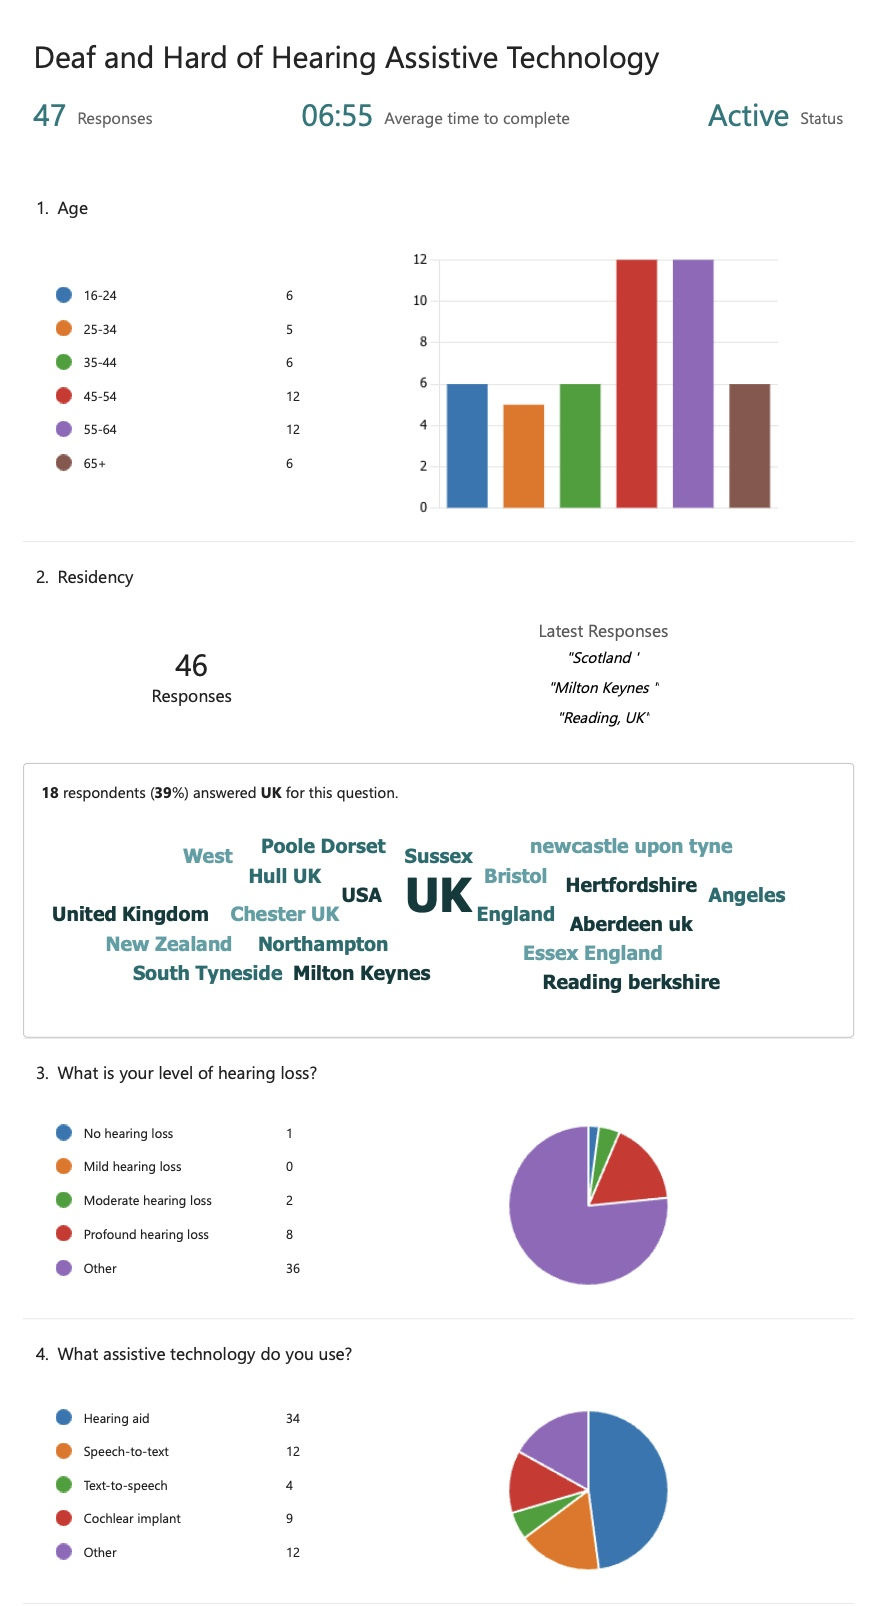
\includegraphics[width=0.60\linewidth]{dissertation/images/afford-survey-1.jpeg}    
    \caption{This screenshots for the responses to the survey outlined in Section \ref{sec:afford-survey}.}
    \label{fig:afford-survey-1} 
\end{figure}

\begin{figure}[H]
    \centering
    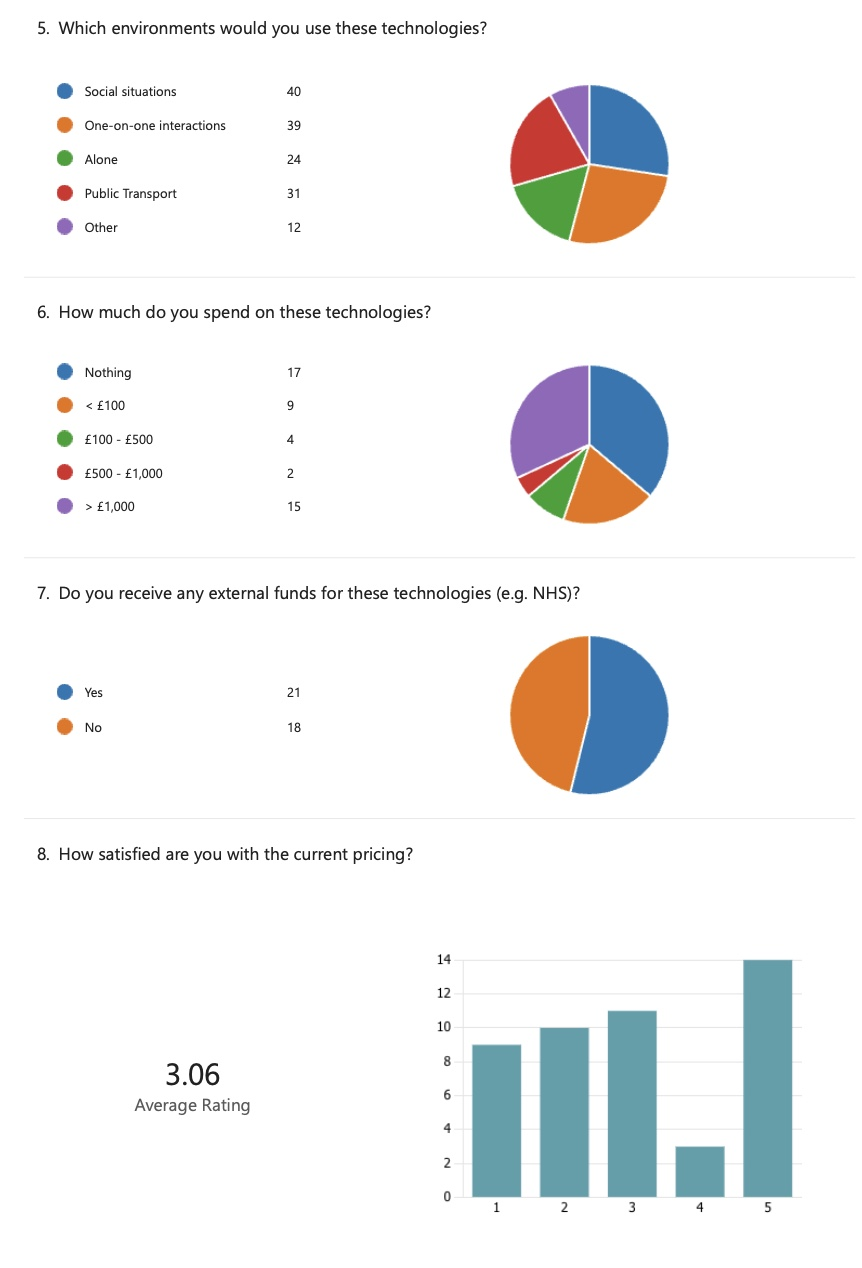
\includegraphics[width=0.75\linewidth]{dissertation/images/afford-survey-2.jpeg}    
    \caption{This screenshots for the responses to the survey outlined in Section \ref{sec:afford-survey}.}
    \label{fig:afford-survey-2} 
\end{figure}

\begin{figure}[H]
    \centering
    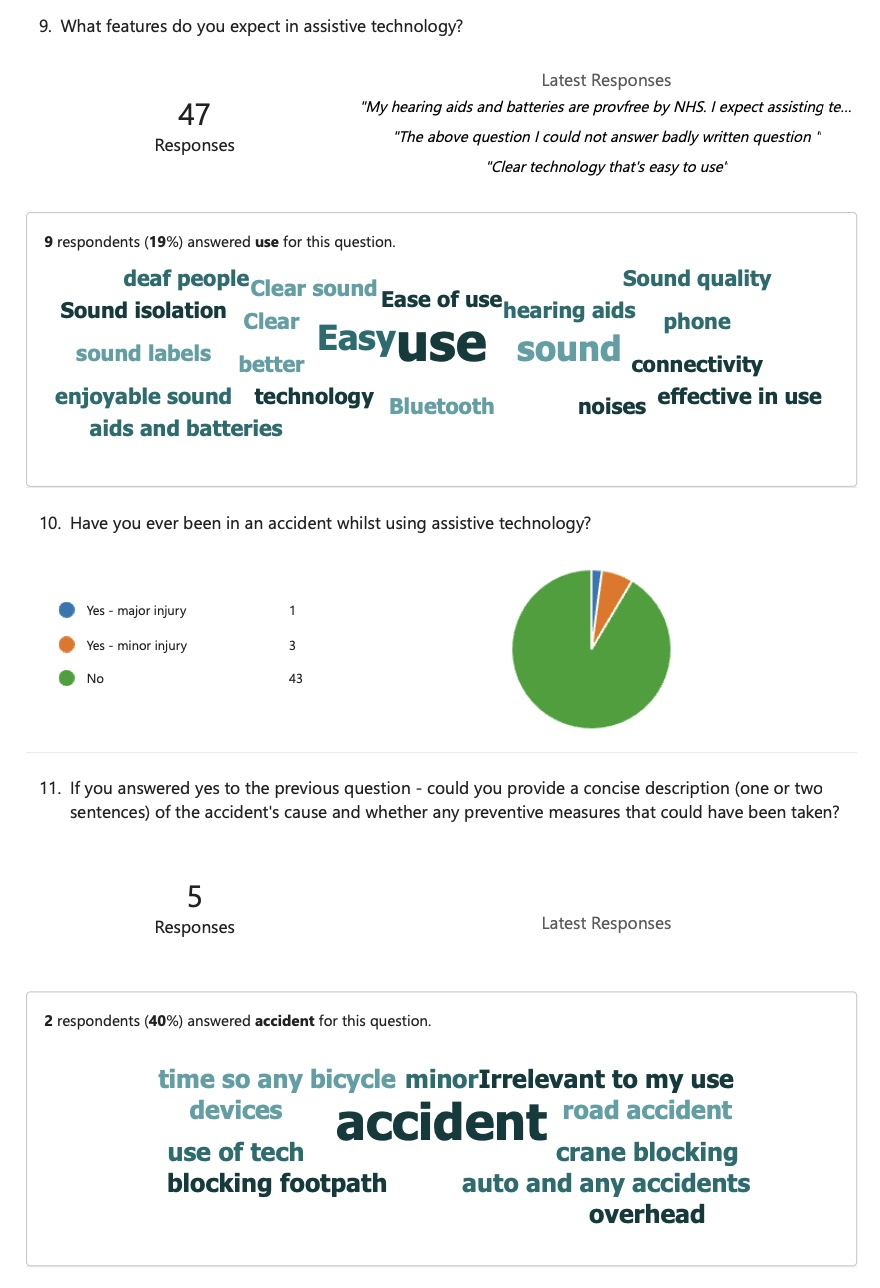
\includegraphics[width=0.75\linewidth]{dissertation/images/afford-survey-3.jpeg}    
    \caption{This screenshots for the responses to the survey outlined in Section \ref{sec:afford-survey}.}
    \label{fig:afford-survey-3} 
\end{figure}

\begin{figure}[H]
    \centering
    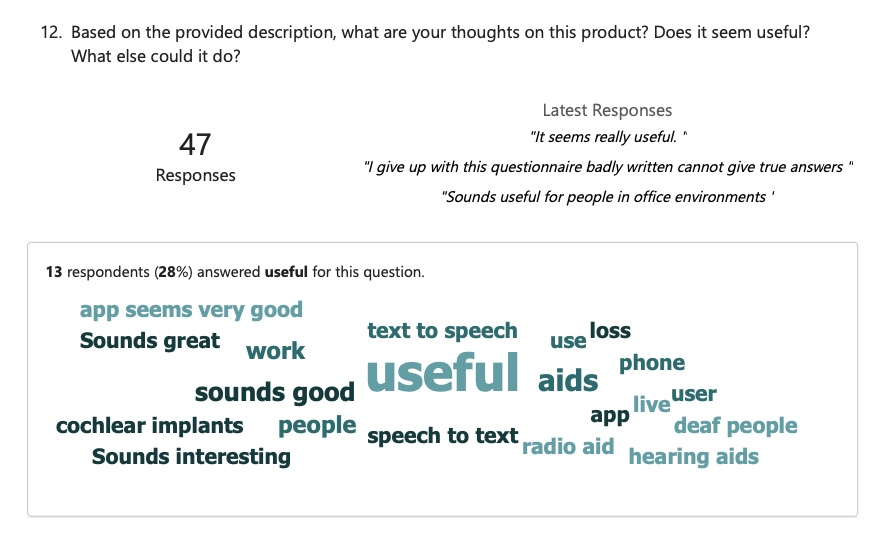
\includegraphics[width=0.75\linewidth]{dissertation/images/afford-survey-4.jpeg}    
    \caption{This screenshots for the responses to the survey outlined in Section \ref{sec:afford-survey}.}
    \label{fig:afford-survey-4} 
\end{figure}

\begin{landscape}
\begin{table}[htbp]
    \caption{This table shows the relations between filter type, frequency, Q value and gain in Web Audio API.}\label{tab:filters}
    \rowcolors{2}{}{gray!3}
    \begin{tabular}{p{3cm}p{6cm}p{4cm}p{4cm}p{4cm}}
    \textbf{Filter Type} & \textbf{Description} & \textbf{Frequency} & \textbf{Q} & \textbf{Gain} \\ 
    Low-pass & Standard second-order resonant lowpass filter with 12dB/octave rolloff. Frequencies below the cutoff pass through; frequencies above it are attenuated. & The cutoff frequency. & Indicates how peaked the frequency is around the cutoff. The greater the value is, the greater is the peak. & Not used \\ 
    High-pass & Standard second-order resonant highpass filter with 12dB/octave rolloff. Frequencies below the cutoff are attenuated; frequencies above it pass through. & The cutoff frequency. & Indicates how peaked the frequency is around the cutoff. The greater the value, the greater the peak. & Not used \\ 
    Band-pass & Standard second-order bandpass filter. Frequencies outside the given range of frequencies are attenuated; the frequencies inside it pass through. & The center of the range of frequencies. & Controls the width of the frequency band. The greater the Q value, the smaller the frequency band. & Not used \\ 
    Lowshelf & Standard second-order lowshelf filter. Frequencies lower than the frequency get a boost, or an attenuation; frequencies over it are unchanged. & The upper limit of the frequencies getting a boost or an attenuation. & Not used & The boost, in dB, to be applied; if negative, it will be an attenuation. \\ 
    Highshelf & Standard second-order highshelf filter. Frequencies higher than the frequency get a boost or an attenuation; frequencies lower than it are unchanged. & The lower limit of the frequencies getting a boost or an attenuation. & Not used & The boost, in dB, to be applied; if negative, it will be an attenuation. \\ 
    Peaking & Frequencies inside the range get a boost or an attenuation; frequencies outside it are unchanged. & The middle of the frequency range getting a boost or an attenuation. & Controls the width of the frequency band. The greater the Q value, the smaller the frequency band. & The boost, in dB, to be applied; if negative, it will be an attenuation. \\ 
    Notch & Standard notch filter, also called a band-stop or band-rejection filter. It is the opposite of a bandpass filter: frequencies outside the give range of frequencies pass through; frequencies inside it are attenuated. & The center of the range of frequencies. & Controls the width of the frequency band. The greater the Q value, the smaller the frequency band. & Not used \\ 
    Allpass & Standard second-order allpass filter. It lets all frequencies through, but changes the phase-relationship between the various frequencies. & The frequency with the maximal group delay, that is, the frequency where the center of the phase transition occurs. & Controls how sharp the transition is at the medium frequency. The larger this parameter is, the sharper and larger the transition will be. & Not used \\ 
    \end{tabular}
\end{table}
\end{landscape}

\begin{figure}[H]
    \centering
    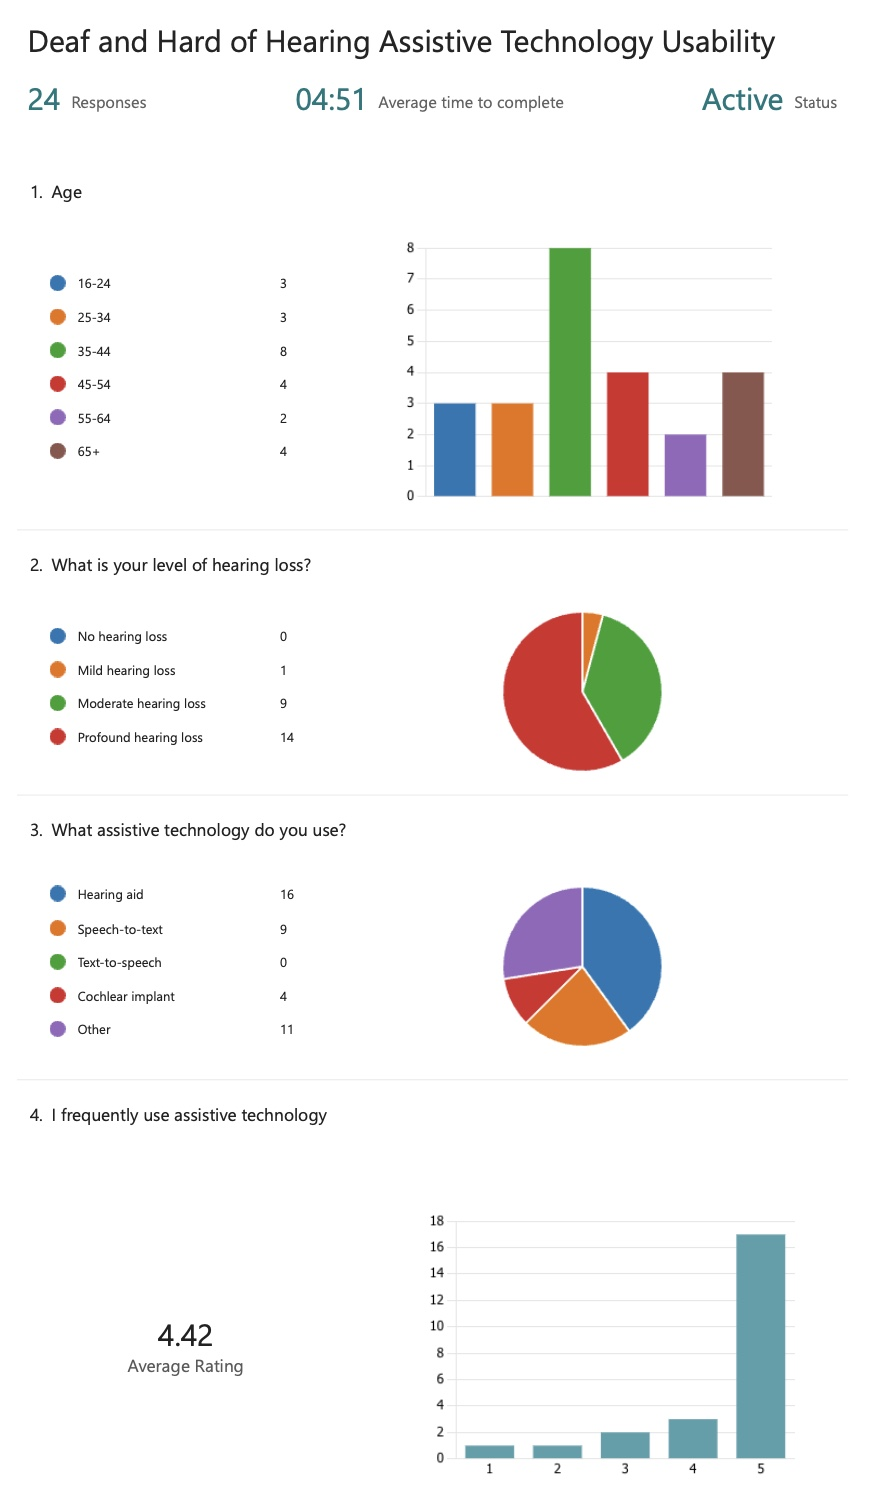
\includegraphics[width=0.75\linewidth]{dissertation/images/use-survey-1.jpeg}    
    \caption{This screenshots for the responses to the survey outlined in Section \ref{sec:use-survey}.}
    \label{fig:use-survey-1} 
\end{figure}

\begin{figure}[H]
    \centering
    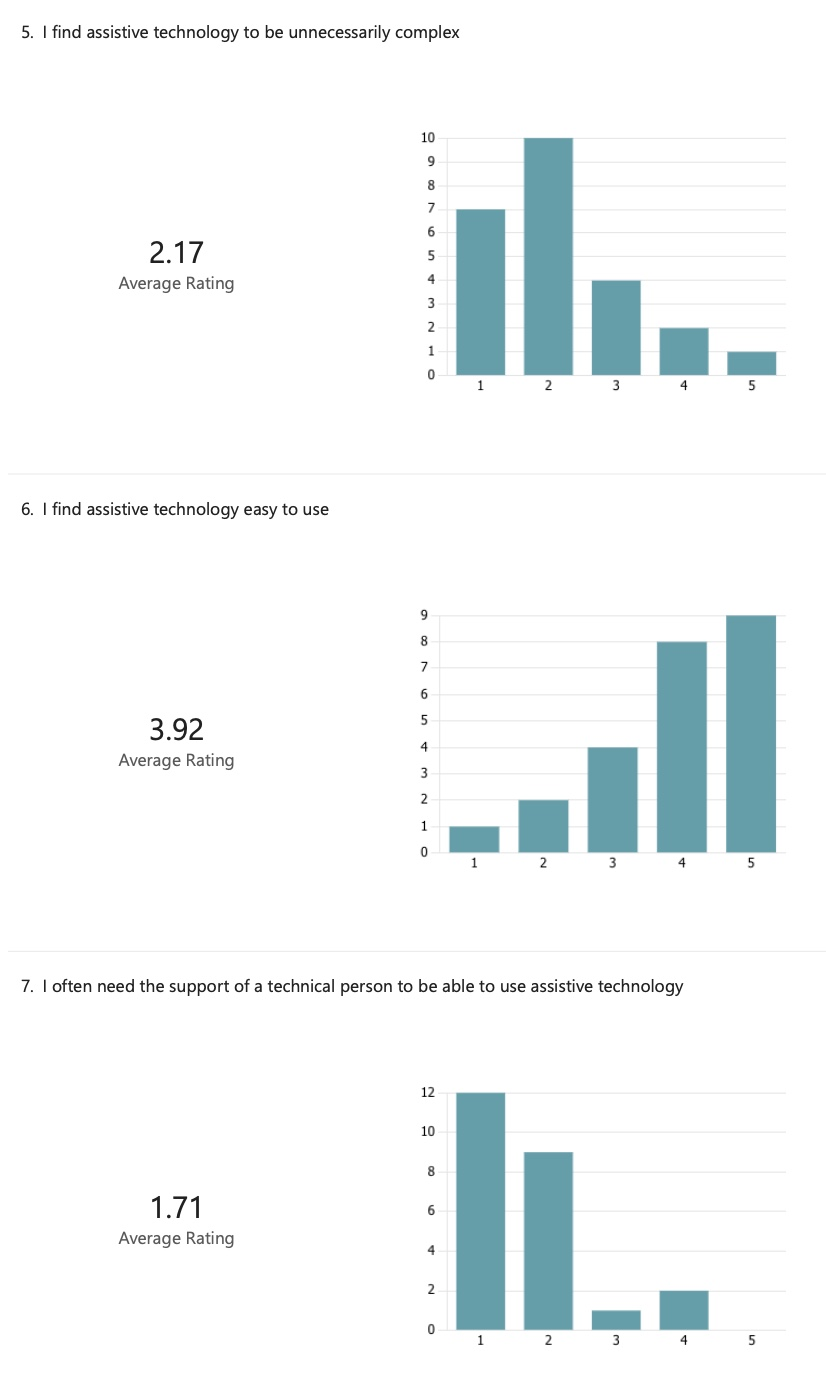
\includegraphics[width=0.75\linewidth]{dissertation/images/use-survey-2.jpeg}    
    \caption{This screenshots for the responses to the survey outlined in Section \ref{sec:use-survey}.}
    \label{fig:use-survey-2} 
\end{figure}

\begin{figure}[H]
    \centering
    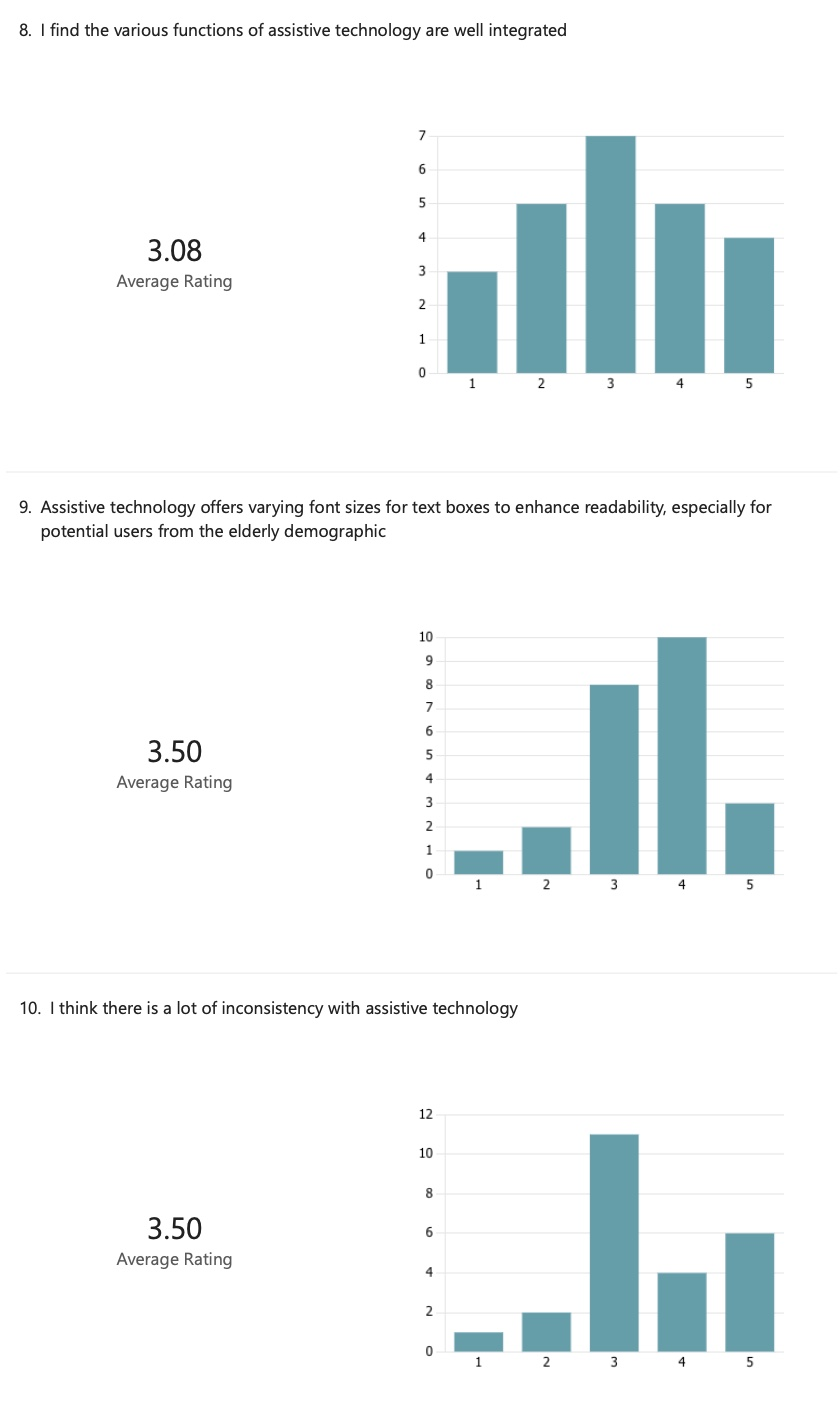
\includegraphics[width=0.75\linewidth]{dissertation/images/use-survey-3.jpeg}    
    \caption{This screenshots for the responses to the survey outlined in Section \ref{sec:use-survey}.}
    \label{fig:use-survey-3} 
\end{figure}

\begin{figure}[H]
    \centering
    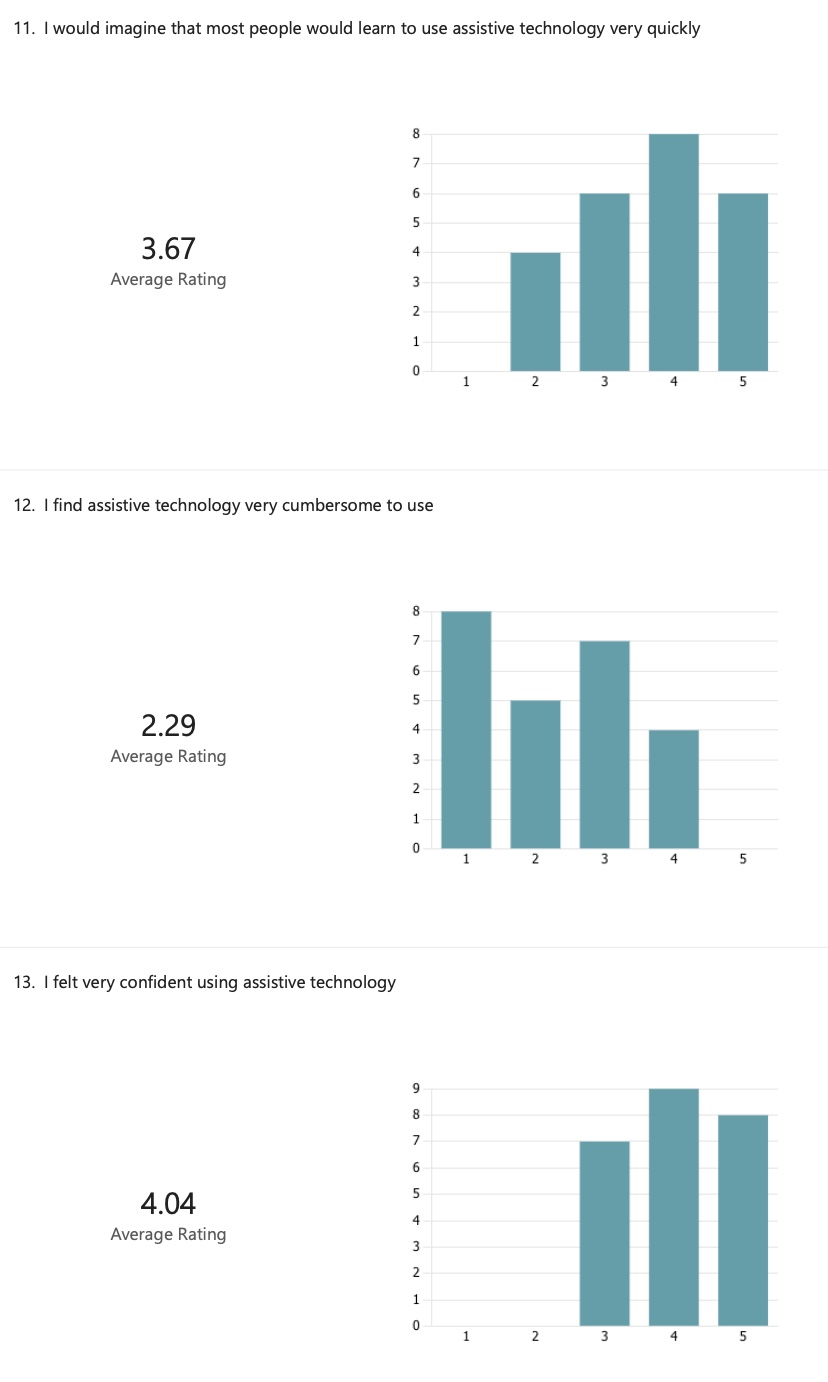
\includegraphics[width=0.75\linewidth]{dissertation/images/use-survey-4.jpeg}    
    \caption{This screenshots for the responses to the survey outlined in Section \ref{sec:use-survey}.}
    \label{fig:use-survey-4} 
\end{figure}

\begin{figure}[H]
    \centering
    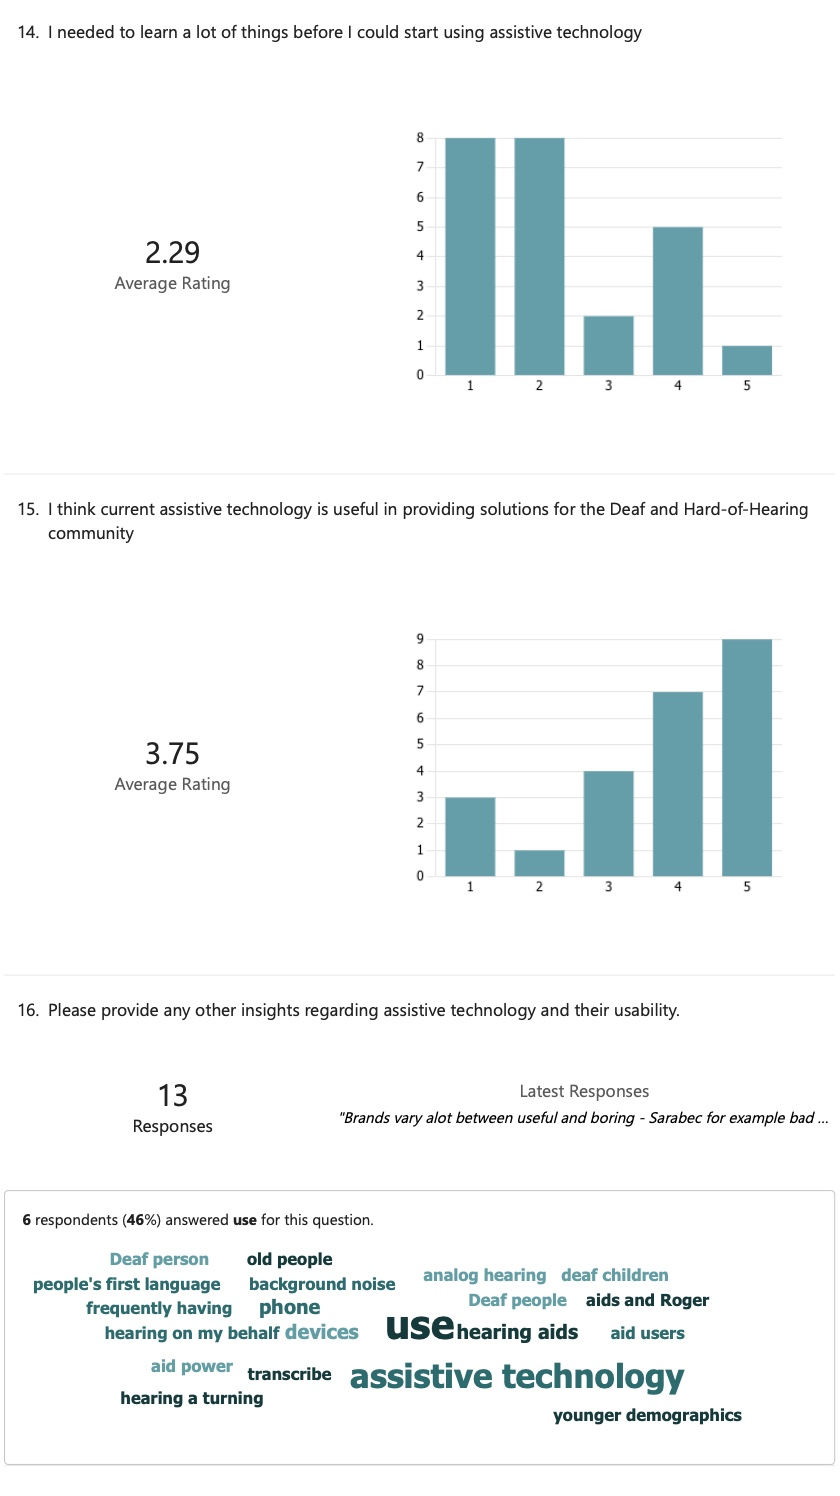
\includegraphics[width=0.75\linewidth]{dissertation/images/use-survey-5.jpeg}    
    \caption{This screenshots for the responses to the survey outlined in Section \ref{sec:use-survey}.}
    \label{fig:use-survey-5} 
\end{figure}

\begin{figure}[H]
    \centering
    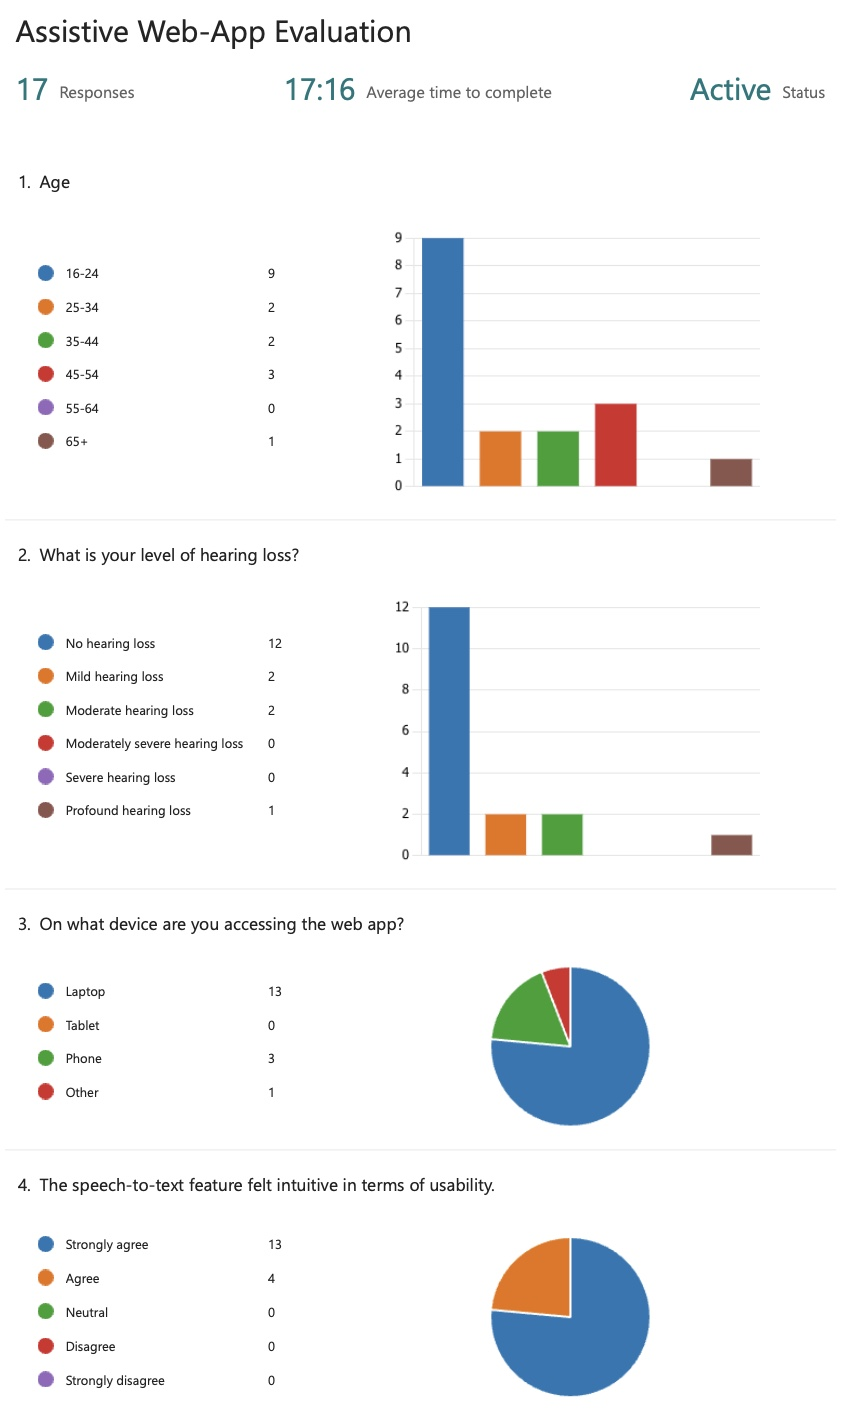
\includegraphics[width=0.75\linewidth]{dissertation/images/eval-1.jpeg}    
    \caption{This screenshots for the responses to the survey outlined in Section \ref{sec:evaluation}.}
    \label{fig:eval-survey-1} 
\end{figure}

\begin{figure}[H]
    \centering
    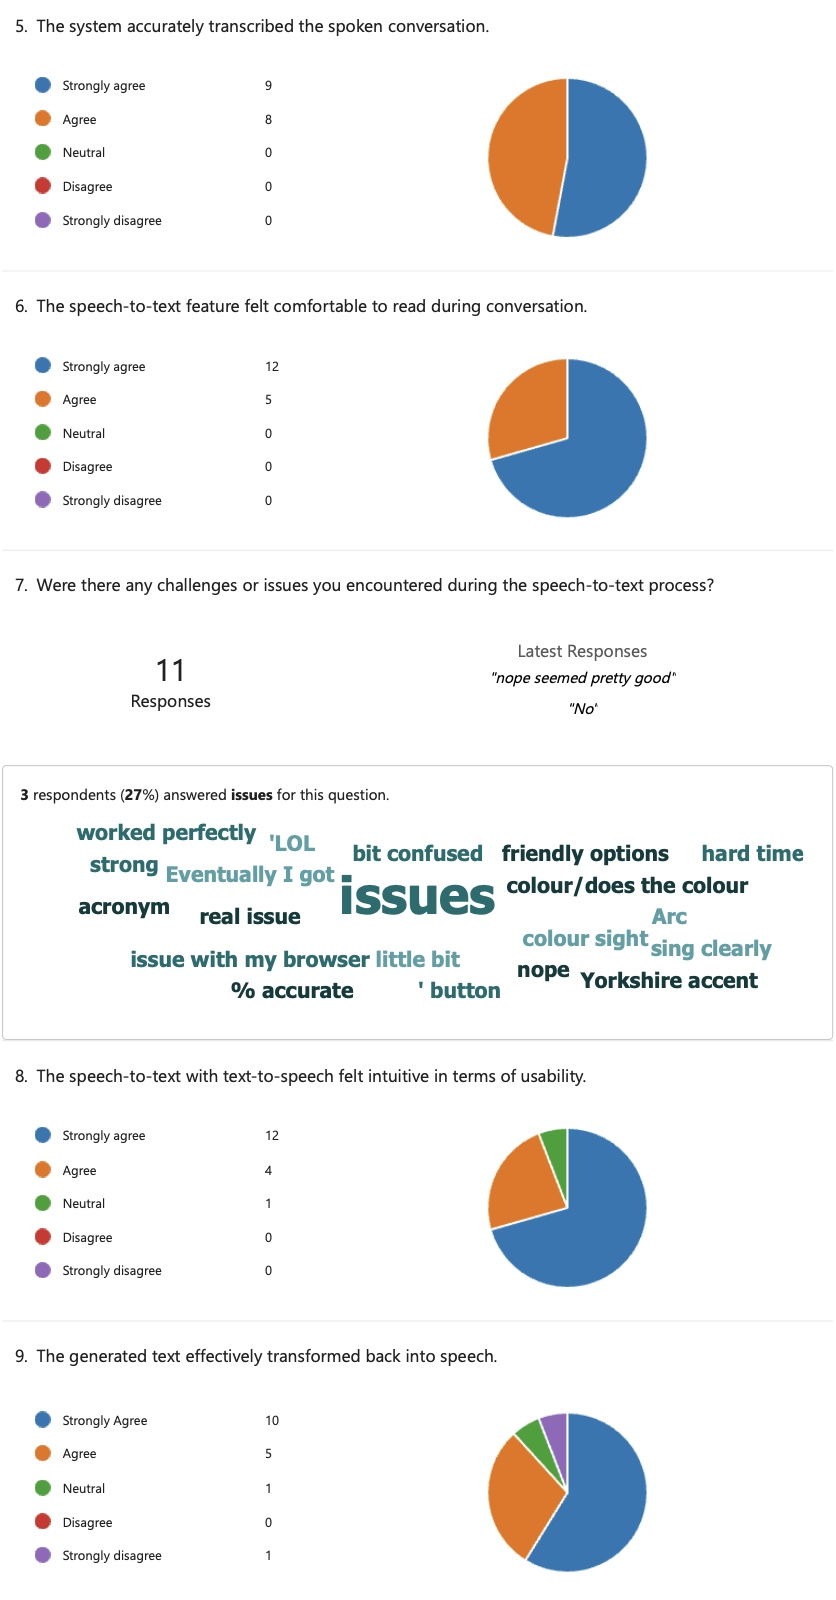
\includegraphics[width=0.75\linewidth]{dissertation/images/eval-2.jpeg}    
    \caption{This screenshots for the responses to the survey outlined in Section \ref{sec:evaluation}.}
    \label{fig:eval-survey-2} 
\end{figure}

\begin{figure}[H]
    \centering
    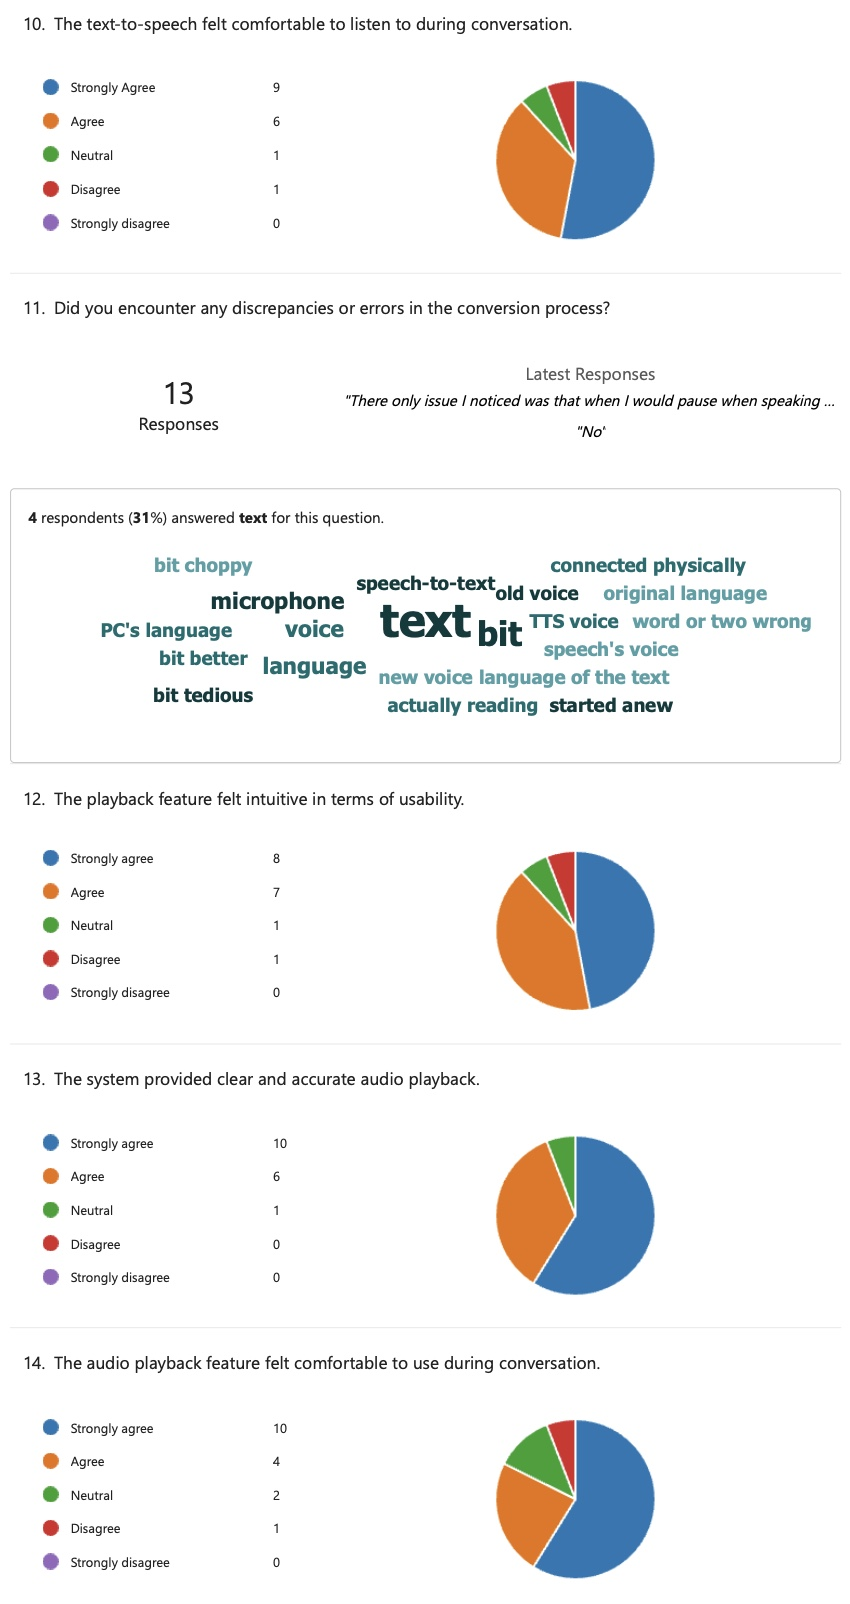
\includegraphics[width=0.75\linewidth]{dissertation/images/eval-3.jpeg}    
    \caption{This screenshots for the responses to the survey outlined in Section \ref{sec:evaluation}.}
    \label{fig:eval-survey-3} 
\end{figure}

\begin{figure}[H]
    \centering
    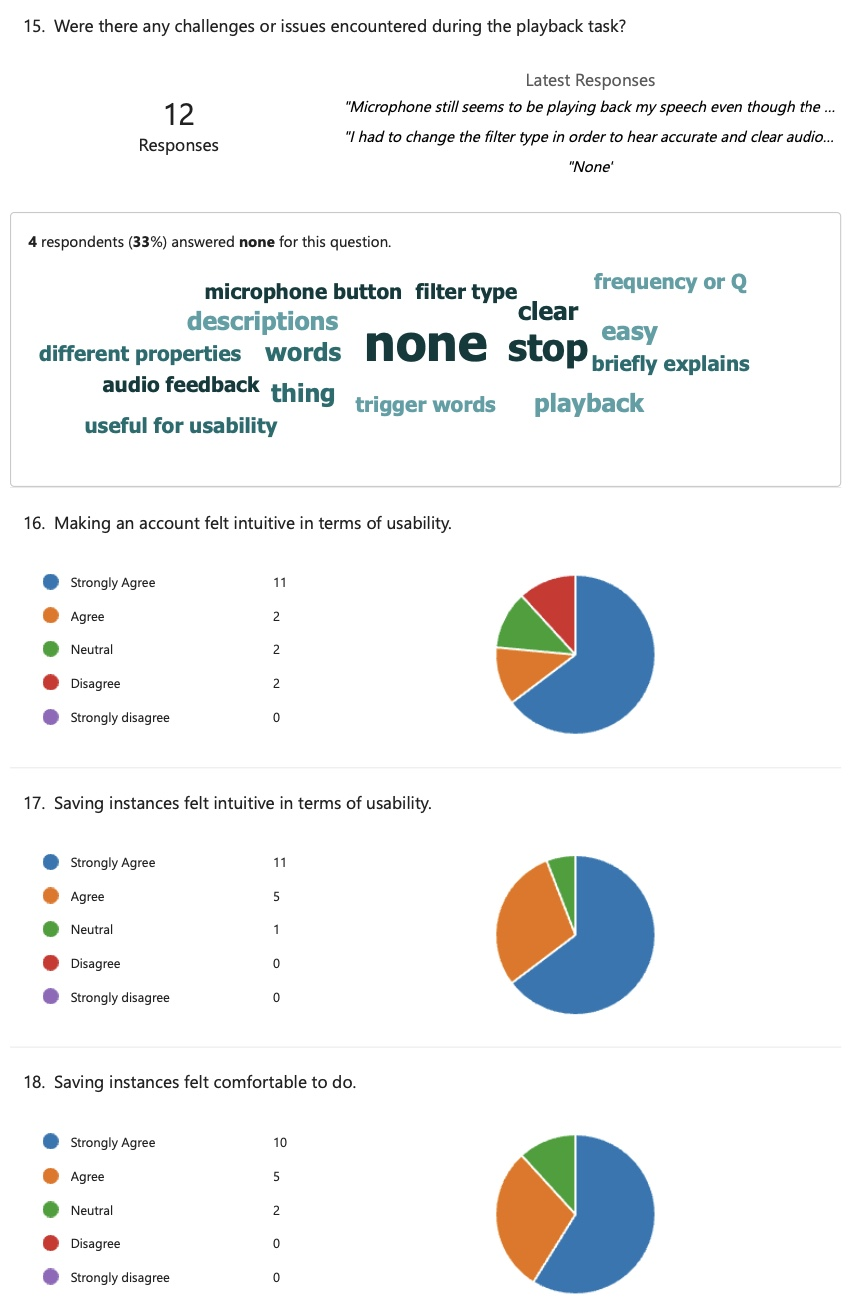
\includegraphics[width=0.75\linewidth]{dissertation/images/eval-4.jpeg}    
    \caption{This screenshots for the responses to the survey outlined in Section \ref{sec:evaluation}.}
    \label{fig:eval-survey-4} 
\end{figure}

\begin{figure}[H]
    \centering
    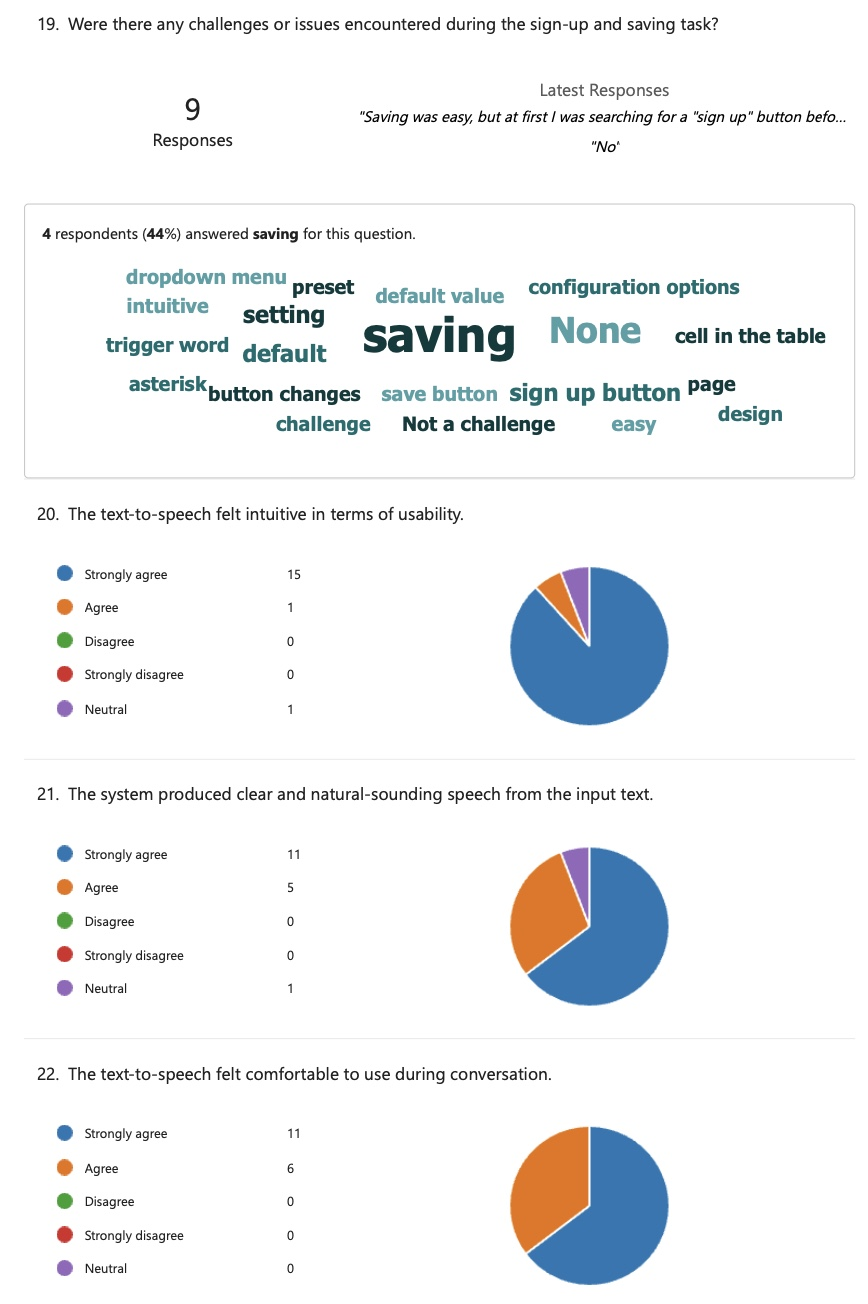
\includegraphics[width=0.75\linewidth]{dissertation/images/eval-5.jpeg}    
    \caption{This screenshots for the responses to the survey outlined in Section \ref{sec:evaluation}.}
    \label{fig:eval-survey-5} 
\end{figure}

\begin{figure}[H]
    \centering
    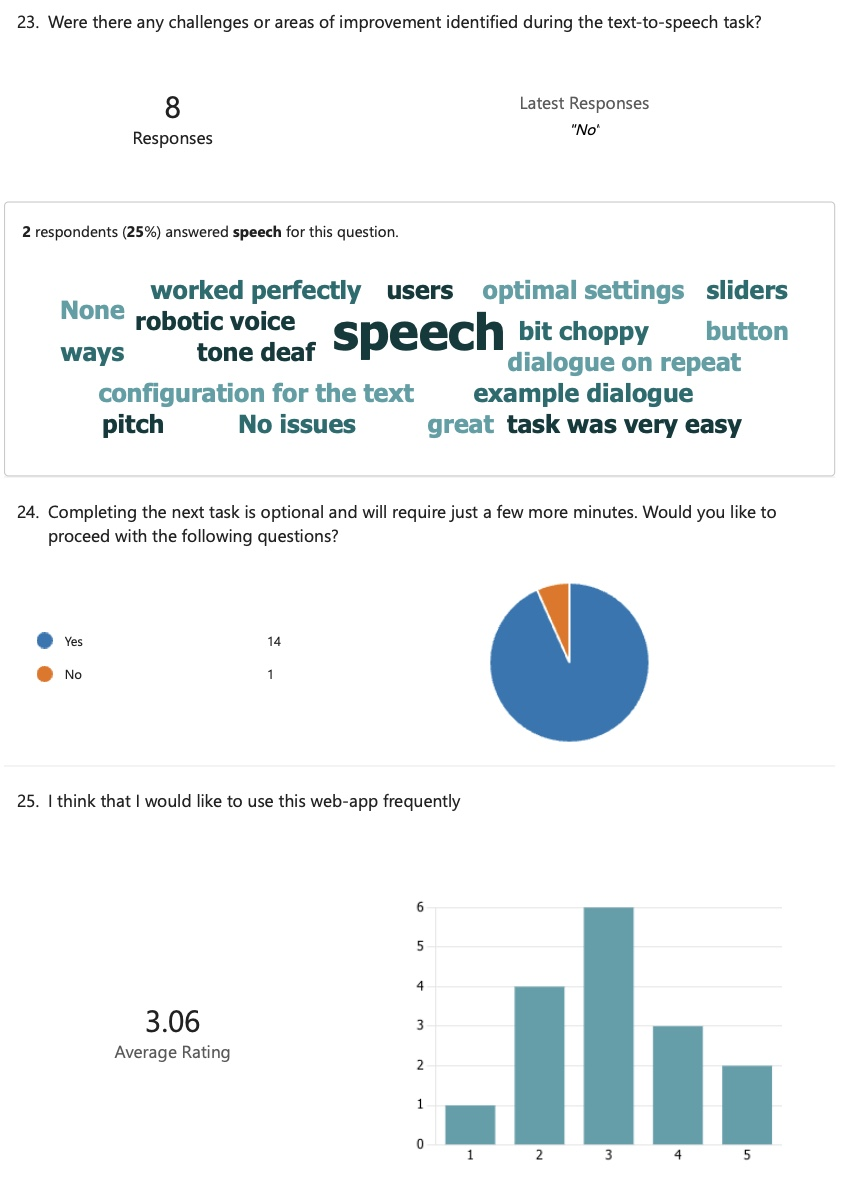
\includegraphics[width=0.75\linewidth]{dissertation/images/eval-6.jpeg}    
    \caption{This screenshots for the responses to the survey outlined in Section \ref{sec:evaluation}.}
    \label{fig:eval-survey-6} 
\end{figure}

\begin{figure}[H]
    \centering
    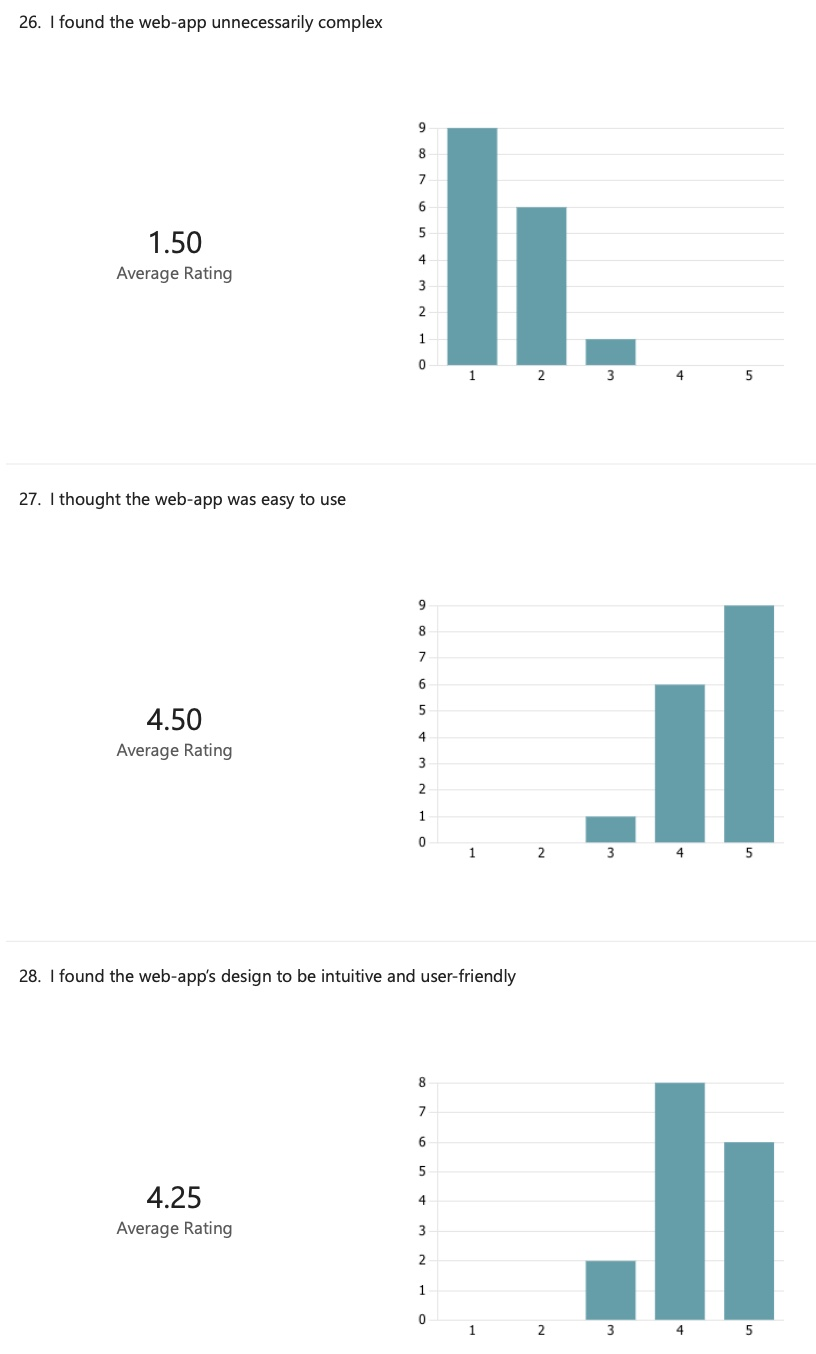
\includegraphics[width=0.75\linewidth]{dissertation/images/eval-7.jpeg}    
    \caption{This screenshots for the responses to the survey outlined in Section \ref{sec:evaluation}.}
    \label{fig:eval-survey-7} 
\end{figure}

\begin{figure}[H]
    \centering
    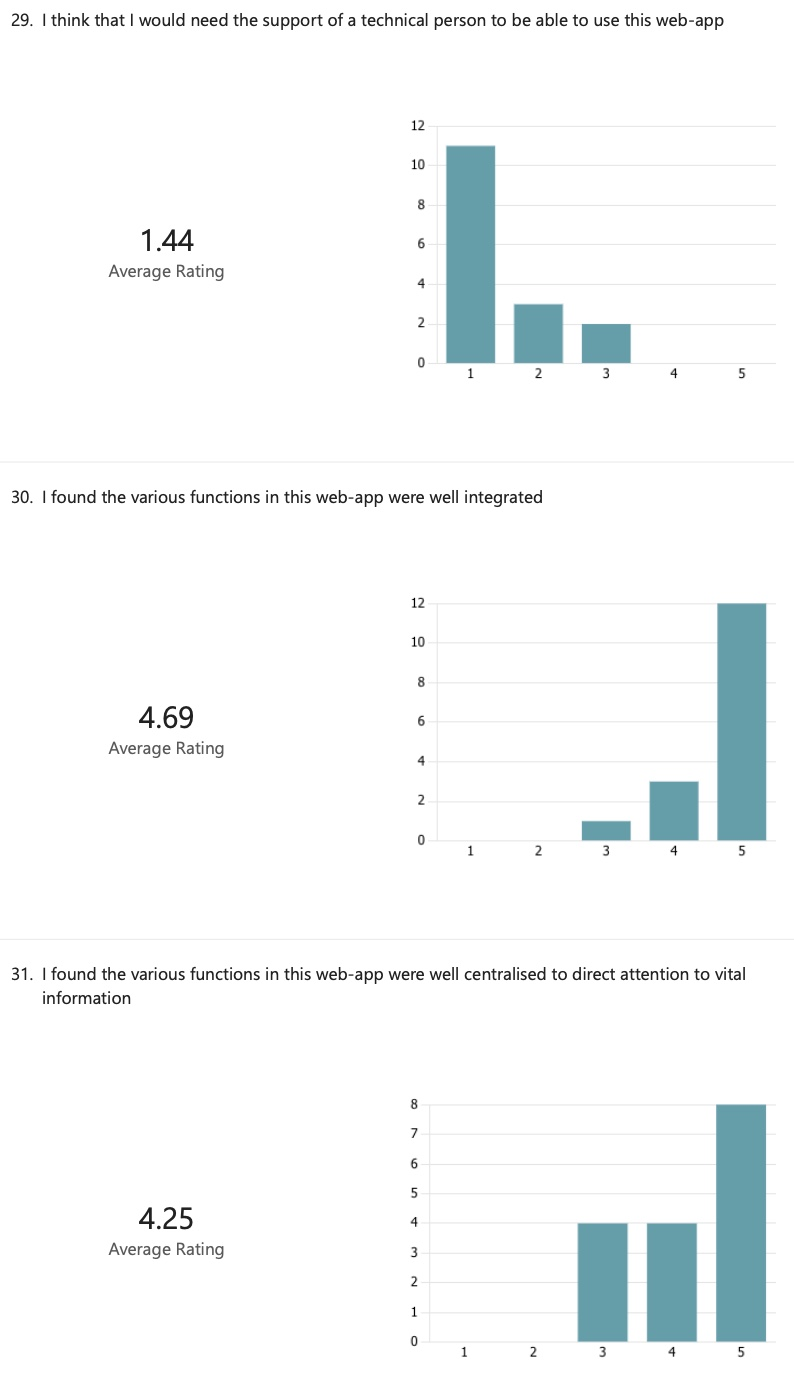
\includegraphics[width=0.75\linewidth]{dissertation/images/eval-8.jpeg}    
    \caption{This screenshots for the responses to the survey outlined in Section \ref{sec:evaluation}.}
    \label{fig:eval-survey-8} 
\end{figure}

\begin{figure}[H]
    \centering
    \includegraphics[width=0.75\linewidth]{dissertation/images/eval-9.jpeg}    
    \caption{This screenshots for the responses to the survey outlined in Section \ref{sec:evaluation}.}
    \label{fig:eval-survey-9} 
\end{figure}

\begin{figure}[H]
    \centering
    \includegraphics[width=0.75\linewidth]{dissertation/images/eval-10.jpeg}    
    \caption{This screenshots for the responses to the survey outlined in Section \ref{sec:evaluation}.}
    \label{fig:eval-survey-10} 
\end{figure}

\begin{figure}[H]
    \centering
    \includegraphics[width=0.75\linewidth]{dissertation/images/eval-11.jpeg}    
    \caption{This screenshots for the responses to the survey outlined in Section \ref{sec:evaluation}.}
    \label{fig:eval-survey-11} 
\end{figure}

\begin{figure}[H]
    \centering
    \includegraphics[width=0.75\linewidth]{dissertation/images/eval-12.jpeg}    
    \caption{This screenshots for the responses to the survey outlined in Section \ref{sec:evaluation}.}
    \label{fig:eval-survey-12} 
\end{figure}

\begin{table}[htbp]
    \caption{This table displays the scores for each question in relation to the UI requirements outlines in Section \ref{sec:UI}, from a scale of 0-4 utilising the same method outlined in Section \ref{sec:evaluation}.}
    \label{tab:UI-table}
    %\tt 
    \rowcolors{2}{}{gray!3}
    \begin{tabular}{@{}lllllllllllllllll@{}}
    %\toprule
    \textbf{Questions} & \textbf{UI.1} & \textbf{UI.2} & \textbf{UI.3} & \textbf{UI.4} & \textbf{UI.5} & \textbf{UI.6} & \textbf{UI.7} \\
    \textbf{1}  & - & - & - & - & - & -& -\\ 
    \textbf{2}  & \checkmark & - & - & - & - &- &- \\ 
    \textbf{3}  & - & -& - & - & - & -& -\\ 
    \textbf{4}  & - & -& - & - & - &- &- \\ 
    \textbf{5}  & - & -& - & - & - & -&- \\ 
    \textbf{6}  & - & -& \checkmark & - & - & -&- \\ 
    \textbf{7}  & - & -& \checkmark & - & - & -&-\\ 
    \textbf{8}  & - & - & - & \checkmark & - & -&-\\
    \textbf{9}  & - & - & - & - & \checkmark & -&-\\
    \textbf{10}  & - & - & - & - & - & \checkmark &-\\
    \textbf{11}  & - & - & - & - & - & -& \checkmark\\
    \textbf{12}  & - & \checkmark & - & \checkmark & - & -&- \\
    \textbf{13}  & - & - & - & - & - &- &- \\
    \textbf{14}  & - & - & - & - & - &- &- \\
    \textbf{15}  & - & - & - & - & - &- &-\\
    \textbf{16}  & - & -& - & - & - &- & -\\
    \textbf{17}  & - & -& - & - & - & -&- \\
    % \bottomrule
\end{tabular}
\end{table}

\begin{table}[htbp]
    \caption{This table displays the scores for each question in relation to the UX requirements outlines in Section \ref{sec:UX}, from a scale of 0-4 utilising the same method outlined in Section \ref{sec:evaluation}.}
    \label{tab:UX-table}
    %\tt 
    \rowcolors{2}{}{gray!3}
    \begin{tabular}{@{}llllllll@{}}
    %\toprule
    \textbf{Questions} & \textbf{UX.1} & \textbf{UX.2} & \textbf{UX.3} & \textbf{UX.4} & \textbf{UX.5} & \textbf{UX.6} & \textbf{UX.7} \\
    \textbf{1}  & - & \checkmark & - & - & - & -& -\\ 
    \textbf{2}  & - & \checkmark & - & - & - &- &- \\ 
    \textbf{3}  & - & \checkmark & - & - & - & -& -\\ 
    \textbf{4}  & - & \checkmark & - & - & - &- &- \\ 
    \textbf{5}  & - & -& - & - & \checkmark & -&- \\ 
    \textbf{6}  & - & \checkmark & - & - & - & -&- \\ 
    \textbf{7}  & - & -& - & \checkmark & - & -&-\\ 
    \textbf{8}  & - & - & \checkmark & - & - & -&-\\
    \textbf{9}  & - & - & - & \checkmark & - & -&-\\
    \textbf{10}  & - & - & - & - & \checkmark & \checkmark &-\\
    \textbf{11}  & - & - & - & - & - & -& -\\
    \textbf{12}  & - & - & - & - & - & -&- \\
    \textbf{13}  & - & \checkmark & - & - & - &- &- \\
    \textbf{14}  & - & \checkmark & - & - & - &- &- \\
    \textbf{15}  & - & \checkmark & - & - & - &- &-\\
    \textbf{16}  & - & \checkmark & - & - & \checkmark &- & -\\
    \textbf{17}  & \checkmark & -& - & - & - & -& \checkmark \\
    % \bottomrule
\end{tabular}
\end{table}

\end{appendices}

%==================================================================================================================================
%   BIBLIOGRAPHY   

% The bibliography style is abbrvnat
% The bibliography always appears last, after the appendices.

\bibliographystyle{abbrvnat}

\bibliography{l4proj}

\end{document}
